\documentclass[SE,lsstdraft,STR,toc]{lsstdoc}
\usepackage{geometry}
\usepackage{longtable,booktabs}
\usepackage{enumitem}
\usepackage{arydshln}

\input meta.tex

\providecommand{\tightlist}{
  \setlength{\itemsep}{0pt}\setlength{\parskip}{0pt}}

\begin{document}

\def\milestoneName{Ccw + Camera Rotator Interface Verification On Camera Cart}
\def\milestoneId{LVV-P58}
\def\product{SIT-COM Integration}

\setDocCompact{true}

\title{ LVV-P58 Ccw + Camera Rotator Interface Verification On Camera Cart Test Plan and Report}
\setDocRef{\lsstDocType-\lsstDocNum}
\date{\vcsdate}
\setDocUpstreamLocation{\url{https://github.com/lsst/lsst-texmf/examples}}
\author{ Austin Roberts }

\input history_and_info.tex


\setDocAbstract{
This is the test plan and report for LVV-P58 (Ccw + Camera Rotator Interface Verification On Camera Cart),
an LSST milestone pertaining to the System Engineering Subsystem.
}


\maketitle

\section{Introduction}
\label{sect:intro}


\subsection{Objectives}
\label{sect:objectives}

The purpose of this test plan is to verify combined control and combined
interlocks of the Camera Rotator integrated with the Camera Cable Wrap
at the Summit facility, as defined in \citeds{LTS-160}, \citeds{LTS-206} and \citeds{LTS-218}. The
combined control will be accomplished through SAL v4.0 utilizing the
LSST pointing component and Jupyter notebooks. This following criteria
must be met in order to execute this test campaign:

\begin{itemize}
\tightlist
\item
  Requires the use of the encoders and a laser tracker only
\item
  Does \textbf{NOT} require the camera rotator to be loaded with the
  camera simulated mass or actual camera hardware
\end{itemize}



\subsection{System Overview}
\label{sect:systemoverview}

The Camera Cable Wrap is mounted to one side of the Integrating
Structure with the Camera Hexapod and Rotator installed on the other
side of the Integrating Structure. This assembly is mounted onto the
Camera Cart when it is off of the telescope. The primary function of the
Camera Cable Wrap is to rotate in a synchronous fashion with the Camera
Rotator to prevent the utilities from getting damaged.


\subsection{Document Overview}
\label{sect:docoverview}

This document was generated from Jira, obtaining the relevant information from the 
\href{https://jira.lsstcorp.org/secure/Tests.jspa#/testPlan/LVV-P58}{LVV-P58}
~Jira Test Plan and related Test Cycles (
  \href{https://jira.lsstcorp.org/secure/Tests.jspa#/testCycle/LVV-C109}{LVV-C109}
).

Section \ref{sect:intro} provides an overview of the test campaign, the system under test (\product{}), the applicable documentation, and explains how this document is organized.
Section \ref{sect:configuration}  describes the configuration used for this test.
Section \ref{sect:personnel} describes the necessary roles and lists the individuals assigned to them.
%Section \ref{sect:plannedtestactivities} provides the list of planned test cycles and test cases, including all relevant information that fully describes the test campaign.

Section \ref{sect:overview} provides a summary of the test results, including an overview in Table \ref{table:summary}, an overall assessment statement and suggestions for possible improvements.
Section \ref{sect:detailedtestresults} provides detailed results for each step in each test case.

The current status of test plan LVV-P58 in Jira is \textbf{ Approved }.

\subsection{References}
\label{sect:references}
\renewcommand{\refname}{}
\bibliography{lsst,refs,books,refs_ads,local}
\section{Test Configuration}
\label{sect:configuration}

\subsection{Data Collection}

  Observing is not required for this test campaign.

\subsection{Verification Environment}
\label{sect:hwconf}
  The Camera Rotator integrated with the Camera Hexapod and Camera Cable
Wrap on the Camera Cart will be verified in a climate controlled
environment on the 3rd floor of the Summit Facility.


  \subsection{Entry Criteria}
  In order to test the Camera Rotator + CCW functionality, the following
criteria must be met first:

\begin{itemize}
\tightlist
\item
  The Camera Rotator's functionality and interlocks have been verified
  to be operational after delivery to the Summit from the vendor
\item
  The Camera Rotator's software has been updated by LSST to be SAL v4.0
  compatible
\item
  The Camera Cable Wrap functionality and interlocks have been verified
  to be operational after delivery to the Summit from the vendor
\item
  The Camera Cable Wrap software has been updated by LSST to be SAL v4.0
  compatible
\end{itemize}


  \subsection{Exit Criteria}
  In order for this event to be considered complete, the following
criteria must be met:

\begin{itemize}
\tightlist
\item
  Raw test data, events, and telemetry have been saved for both the
  Camera Rotator and the CCW.
\item
  All test data has been analyzed and post processed.
\item
  All test steps have been statused in the Jira Test Cases within this
  Test Plan and actual results populated as required.
\item
  A summary of the results of the test campaign has been captured in the
  Overall Assessment and Recommended Improvements fields of this Test
  Plan
\item
  A link to the verification artifacts used to produce the summary of
  results has been populated in the Verification Artifacts field of this
  Test Plan
\item
  Any failures have been captured in the
  \href{https://jira.lsstcorp.org/projects/FRACAS/issues/}{FRACAS}
  project
\end{itemize}


  \subsection{PMCS Activity}
  See Epics in Traceability Tab


\newpage
\section{Personnel}
\label{sect:personnel}

The personnel involved in the test campaign is shown in the following table.

\begin{longtable}{p{3cm}p{3cm}p{3cm}p{6cm}}
\hline
\multicolumn{2}{r}{Test Plan (LVV-P58) owner:} &
\multicolumn{2}{l}{\textbf{ Austin Roberts } }\\\hline
\multicolumn{2}{r}{ LVV-C109 owner:} &
\multicolumn{2}{l}{\textbf{
    Austin Roberts
}
} \\\hline
\textbf{Test Case} & \textbf{Assigned to} & \textbf{Executed by} & \textbf{Additional Test Personnel} \\ \hline
\href{https://jira.lsstcorp.org/secure/Tests.jspa#/testCase/LVV-T1602}{LVV-T1602}
& {\small Kevin Siruno } & {\small Kevin Siruno } &
\begin{minipage}[]{6cm}
\smallskip
{\small (1) Software Engineer\\
(1) Hardware Engineer
 }
\medskip
\end{minipage}
\\ \hline
\href{https://jira.lsstcorp.org/secure/Tests.jspa#/testCase/LVV-T1569}{LVV-T1569}
& {\small Kevin Siruno } & {\small Kevin Siruno } &
\begin{minipage}[]{6cm}
\smallskip
{\small (1) Software Engineer\\
(1) Hardware Engineer\\
(1) Systems Engineer
 }
\medskip
\end{minipage}
\\ \hline
\href{https://jira.lsstcorp.org/secure/Tests.jspa#/testCase/LVV-T1588}{LVV-T1588}
& {\small Kevin Siruno } & {\small Kevin Siruno } &
\begin{minipage}[]{6cm}
\smallskip
{\small (1) Software Engineer\\
(1) Hardware Engineer\\
(1) Systems Engineer
 }
\medskip
\end{minipage}
\\ \hline
\end{longtable}

\newpage

\section{Test Campaign Overview}
\label{sect:overview}

\subsection{Summary}
\label{sect:summarytable}

\begin{longtable}{p{2cm}p{2.5cm}p{9cm}p{2.5cm}}
\toprule
\multicolumn{3}{l}{ Test Plan {\bf LVV-P58: CCW + Camera Rotator Interface Verification on Camera Cart
 }} & Approved \\\hline

  \multicolumn{3}{l}{ Test Cycle {\bf LVV-C109: Camera Rotator + CCW Integration
 }} & Done \\\hline

  {\bf \footnotesize test case} & {\bf \footnotesize status} & {\bf \footnotesize comment} & {\bf \footnotesize issues} \\\toprule

    \href{https://jira.lsstcorp.org/secure/Tests.jspa#/testCase/LVV-T1602}{LVV-T1602}
    & Fail &
    \begin{minipage}[]{9cm}
    \smallskip
    
    \medskip
    \end{minipage}
    &
          \href{https://jira.lsstcorp.org/browse/LVV-18471}{LVV-18471}
          \href{https://jira.lsstcorp.org/browse/LVV-18474}{LVV-18474}
          \href{https://jira.lsstcorp.org/browse/LVV-18474}{LVV-18474}
          \href{https://jira.lsstcorp.org/browse/LVV-18474}{LVV-18474}
    \\\hline
    \href{https://jira.lsstcorp.org/secure/Tests.jspa#/testCase/LVV-T1569}{LVV-T1569}
    & Fail &
    \begin{minipage}[]{9cm}
    \smallskip
    
    \medskip
    \end{minipage}
    &
          \href{https://jira.lsstcorp.org/browse/LVV-18473}{LVV-18473}
          \href{https://jira.lsstcorp.org/browse/LVV-18473}{LVV-18473}
          \href{https://jira.lsstcorp.org/browse/LVV-18475}{LVV-18475}
          \href{https://jira.lsstcorp.org/browse/LVV-18476}{LVV-18476}
          \href{https://jira.lsstcorp.org/browse/LVV-18473}{LVV-18473}
          \href{https://jira.lsstcorp.org/browse/LVV-18473}{LVV-18473}
          \href{https://jira.lsstcorp.org/browse/LVV-18477}{LVV-18477}
          \href{https://jira.lsstcorp.org/browse/LVV-18477}{LVV-18477}
          \href{https://jira.lsstcorp.org/browse/LVV-18476}{LVV-18476}
          \href{https://jira.lsstcorp.org/browse/LVV-18473}{LVV-18473}
          \href{https://jira.lsstcorp.org/browse/LVV-18473}{LVV-18473}
    \\\hline
    \href{https://jira.lsstcorp.org/secure/Tests.jspa#/testCase/LVV-T1588}{LVV-T1588}
    & Fail &
    \begin{minipage}[]{9cm}
    \smallskip
    
    \medskip
    \end{minipage}
    &
          \href{https://jira.lsstcorp.org/browse/LVV-18478}{LVV-18478}
          \href{https://jira.lsstcorp.org/browse/LVV-18478}{LVV-18478}
          \href{https://jira.lsstcorp.org/browse/LVV-18473}{LVV-18473}
          \href{https://jira.lsstcorp.org/browse/LVV-18473}{LVV-18473}
          \href{https://jira.lsstcorp.org/browse/LVV-18478}{LVV-18478}
          \href{https://jira.lsstcorp.org/browse/LVV-18478}{LVV-18478}
          \href{https://jira.lsstcorp.org/browse/FRACAS-26}{FRACAS-26}
          \href{https://jira.lsstcorp.org/browse/FRACAS-26}{FRACAS-26}
          \href{https://jira.lsstcorp.org/browse/FRACAS-26}{FRACAS-26}
          \href{https://jira.lsstcorp.org/browse/FRACAS-26}{FRACAS-26}
    \\\hline
\caption{Test Results Summary}
\label{table:summary}
\end{longtable}

\subsection{Overall Assessment}
\label{sect:overallassessment}

Overall, the result of the test campaign was a FAIL as each test case in
this event had a failure that needs to be
fixed.\\[2\baselineskip]\emph{Integration of Camera Rotator with SAL 4.0
(LSST)} - Nearly all of the Camera Rotator software requirements were
successfully re-verified using LSST's CSC. The only failed test steps
were the test sequences involving the \emph{trackStart~}and
\emph{track~}command. The Camera Rotator was not sent into a FAULT state
as expected when given a \emph{trackStart~}without a
\emph{track~}command immediately after. Instead, the trajectory of the
\emph{trackStart} command would continue to internally calculate the
original command and the track history was required to be cleared for
the trajectory of another \emph{trackStart} command to be
calculated.\\[2\baselineskip]\emph{Integrated CCW + HR Interlock Test~}-
This test case failed because the positive and negative limit switches
on the Synchronous motion assembly were not tripped at +/-2.2 degrees,
as required. Instead, the limit switches were found to be at +2.7degrees
and -5.19 degrees. Furthermore, to reset the Synchronous Motion
interlocks, the CCW had to be at -0.5degrees to clear the Synchronous
motion assembly's positive limit switch. We believe if we adjust the
limit switches to the correct position, we would not be able to clear
both the positive and negative limit switches due to the hysteresis in
the limit switch mechanism and the angle and width of the slope on the
CAM.\\[2\baselineskip]\emph{Pointing Component Control Test -~}Out of
the four scenarios that were tested in this test case, the Basic Control
Scenario was the only test that passed. There were issues that were
discovered during the \emph{High Rotation Stress Test, Filter Change
Scenario,~}and \emph{Typical Night Scenario.}\\
During the \emph{High Rotation Stress Test,~}the Camera Rotator and CCW
both followed the initial track to +90 degrees. However, when a new
track of -90 degrees was sent, the Camera Rotator GUI crashed and the
system went into a FAULT state as the CCW tripped the interlock by
moving out of sync from the Camera Rotator. We had to modify the test to
include a stationary \emph{track} to -90 degrees from +90 degrees
instead of a~\emph{move} command to -90 degrees from +90 degrees.\\
During the \emph{Filter Change Scenario,~}the Camera Rotator and CCW
moved synchronously to follow the initial \emph{track} command, but a
\emph{stop} command had to be issued to the CCW immediately after a
\emph{stopTracking} command was sent to the pointing component to avoid
sending the system into a FAULT state. Furthermore, the Camera Rotator
and CCW needed to be sent to zero degrees using a \emph{track~}command
since the CCW does not subscribe to any \emph{move~}commands sent to the
Camera Rotator.\\
During the \emph{Typical Night Scenario,~}there were more problems with
the Camera GUI crashing. The integrated system was only able to move
together through (at most) three visits during the 5th attempt before
the Camera Rotator GUI crashed again.~


\subsection{Recommended Improvements}
\label{sect:recommendations}

The following action items were generated in order to improve the
system:

\begin{itemize}
\tightlist
\item
  {[}Camera Rotator{]} Add SAL command acknowledgement
\item
  {[}Camera Rotator{]} Update the logging messages of the Camera Rotator
  GUI so that it is easier to read
\item
  {[}Camera Rotator{]} {Update the new rotator CSC to allow changes to
  be made to the configuration file}
\item
  {[}Camera Rotator{]} Update tracking in Simulink model for following
  issues

  \begin{itemize}
  \tightlist
  \item
    High peaks have been seen in transition between two different target
    tracks
  \item
    Previous track history is not cleared in between tracks
  \item
    No rejection for out-of-range track command calculated in Simulink
  \item
    Stop command was needed to allow for multiple tracking
  \end{itemize}
\item
  {[}Camera Rotator{]} Fix Camera Rotator GUI crashing issue
\item
  {[}CCW{]} Change the +/-2.2 degrees limit to a software limit and
  relocate the hardware limit switches to \textbf{TBD~}position to
  protect the utility lines
\item
  {[}CCW{]} Include the ability to move synchronously without tracking
\item
  {[}CCW{]} Review SAL command set i.e. positionSet, move,
  configureVelocity, configureAcceleration
\item
  {[}CCW{]} Update to use callback method over the current polling
  method
\item
  {[}CCW{]} Fix for proper acknowledgements of commands
\item
  {[}CCW{]} Determine whether the EUI should be able to take control
  back from SAL at ANY state or only in some states
\item
  {[}CCW{]} Add Park and Stow Command
\item
  {[}CCW{]} Configure the EFD at Tekniker's site to have a teststand
  environment that has all components that will be used on the summit to
  operate the CCW and Camera Rotator
\end{itemize}


\newpage
\section{Detailed Test Results}
\label{sect:detailedtestresults}

\subsection{Test Cycle LVV-C109 }

Open test cycle {\it \href{https://jira.lsstcorp.org/secure/Tests.jspa#/testrun/LVV-C109}{Camera Rotator + CCW Integration
}} in Jira.

Camera Rotator + CCW Integration
\\
Status: Done

This test cycle will encompass all the test cases pertaining to the
testing of the CCW Integration with the Camera rotator and the camera
cart.


\subsubsection{Software Version/Baseline}
Not provided.

\subsubsection{Configuration}
Not provided.

\subsubsection{Test Cases in LVV-C109 Test Cycle}

\paragraph{Test Case LVV-T1602 - Integration of Camera Rotator with SAL 4.0 (LSST)
 }\mbox{}\\

Open  \href{https://jira.lsstcorp.org/secure/Tests.jspa#/testCase/LVV-T1602}{\textit{ LVV-T1602 } }
test case in Jira.

The objective of this test case is to verify the software requirements
of the camera rotator, as defined in \citeds{LTS-160} \& \citeds{LTS-206}, utilizing
Russell Owen's code. This test case will only exercise the functionality
that was executed previously and meets the following criteria:

\begin{itemize}
\tightlist
\item
  Only requires the camera rotator to be operable
\item
  Only requires command through the CSC after the cRIO is switched from
  GUI mode to DDS mode
\item
  Does \textbf{NOT~}require the rotator to be loaded with the camera
  simulated mass or actual camera hardware
\end{itemize}

The software functional requirements were previously re-verified during
a test campaign at the Summit without the use of SAL. This test is meant
to confirm that the Camera Rotator is functioning correctly with SAL 4.0
using Russel's new rotator CSC code based on salobj. The test procedure
used during the previous testing without SAL was the \emph{LSST
Hexapods-Rotator Software Acceptance Test Procedure.~}The test steps of
this test case are taken directly from that document on how to perform
the test in a similar way with the use of SAL.\\[2\baselineskip]See the
\emph{New Rotator CSC Test in SLAC at 10/17/2019~}linked in the
Traceability tab for the results of Russel's test of the events and
telemetry with the bare rotator in SLAC.\\[2\baselineskip]See the
attached \emph{LSST Rotator Operator's Manual} for more information on
how to operate the rotator.\\[2\baselineskip]


\textbf{ Preconditions}:\\
Prior to the execution of this test case, the following Summit tasks
must be completed:

\begin{itemize}
\tightlist
\item
  The functional testing of the Camera Rotator Hardware~

  \begin{itemize}
  \tightlist
  \item
    h\href{https://jira.lsstcorp.org/browse/SUMMIT-3370}{ttps://jira.lsstcorp.org/browse/SUMMIT-3370}
  \end{itemize}
\item
  The functional testing of the Camera Rotator Software without SAL

  \begin{itemize}
  \tightlist
  \item
    \url{https://jira.lsstcorp.org/browse/SUMMIT-3371}
  \end{itemize}
\item
  The Camera rotator has been connected to the electronics cabinets and
  the connections have been tested

  \begin{itemize}
  \tightlist
  \item
    \url{https://jira.lsstcorp.org/browse/SUMMIT-3294}
  \end{itemize}
\item
  The Hexapod and Rotator have been installed on camera cart

  \begin{itemize}
  \tightlist
  \item
    \url{https://jira.lsstcorp.org/browse/SUMMIT-3224}
  \end{itemize}
\item
  The cables and cabinets have been checked

  \begin{itemize}
  \tightlist
  \item
    \url{https://jira.lsstcorp.org/browse/SUMMIT-3231}
  \end{itemize}
\end{itemize}


Execution status: {\bf Fail }

Final comment:\\


Detailed steps results:

\begin{longtable}{p{1cm}p{15cm}}
\hline
{Step} & Step Details\\ \hline
1 & Description \\
 & \begin{minipage}[t]{15cm}
{\footnotesize
\smallskip
\textbf{STARTING THE EUI}\\[2\baselineskip]Double click the Hexapod GUI
Viewer desktop icon on the computer.

\begin{itemize}
\tightlist
\item
  This can be done on the Dell Management PC or another computer on the
  same network
\end{itemize}

\medskip }
\end{minipage}
\\ \cdashline{2-2}


 & Expected Result \\
 & \begin{minipage}[t]{15cm}{\footnotesize
\smallskip
A prompt to enter a password is shown.~

\medskip }
\end{minipage} \\ \cdashline{2-2}

 & Actual Result \\
 & \begin{minipage}[t]{15cm}{\footnotesize
\smallskip
The GUI was used from another computer on the same network.

\medskip }
\end{minipage} \\ \cdashline{2-2}

 & Status: \textbf{ Initial Pass } \\ \hline

2 & Description \\
 & \begin{minipage}[t]{15cm}
{\footnotesize
\smallskip
Enter the password ``lsst-vnc''

\begin{itemize}
\tightlist
\item
  If the EUI isn't automatically up and running when the VNC opens,
  double click on the CAM\_Hex\_eGUI or M2\_Hex\_eGUI icon on the VNC
  viewer
\end{itemize}

\medskip }
\end{minipage}
\\ \cdashline{2-2}


 & Expected Result \\
 & \begin{minipage}[t]{15cm}{\footnotesize
\smallskip
The EUI is in the Offline State/PublishOnly substate and is able to
publish through SAL but cannot receive commands.

\medskip }
\end{minipage} \\ \cdashline{2-2}

 & Actual Result \\
 & \begin{minipage}[t]{15cm}{\footnotesize
\smallskip
The EUI was unable to receive SAL commands in the Offline
State/PublishOnly

\medskip }
\end{minipage} \\ \cdashline{2-2}

 & Status: \textbf{ Initial Pass } \\ \hline

3 & Description \\
 & \begin{minipage}[t]{15cm}
{\footnotesize
\smallskip
\textbf{OFFLINESTATE/AVAILABLESTATE}\\
On the Main tab, select the ``Offline SubState Cmd'' field in the
Commands to Send section, set the Offline SubState Triggers to ``System
Ready'' and click on the Send Command button.\\
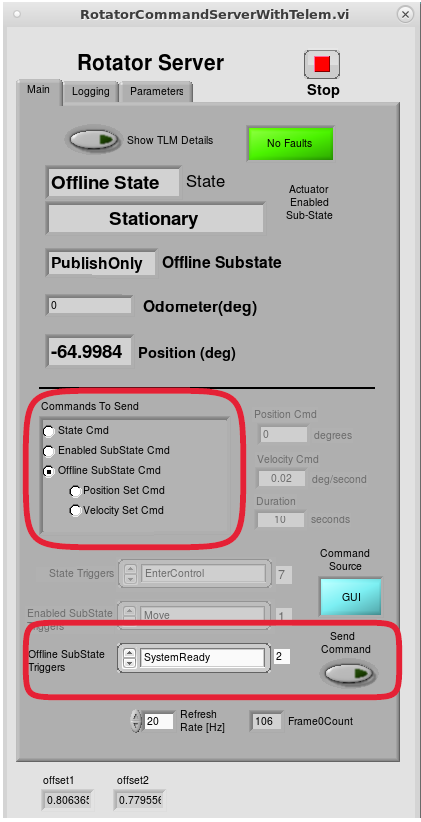
\includegraphics[width=1.79167in]{jira_imgs/1005.png}

\medskip }
\end{minipage}
\\ \cdashline{2-2}


 & Expected Result \\
 & \begin{minipage}[t]{15cm}{\footnotesize
\smallskip
The system transitions from the OfflineState/PublishOnly substate to the
OfflineState/AvailableState
substate.\\[2\baselineskip]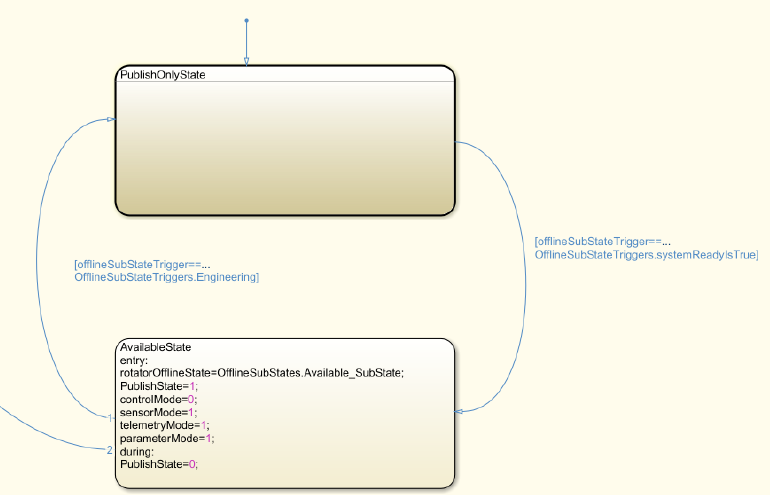
\includegraphics[width=1.79167in]{jira_imgs/1007.png}

\medskip }
\end{minipage} \\ \cdashline{2-2}

 & Actual Result \\
 & \begin{minipage}[t]{15cm}{\footnotesize
\smallskip
In the OfflineState/AvailableState substate, the system was able to
receive/respond to DDS commands.

\medskip }
\end{minipage} \\ \cdashline{2-2}

 & Status: \textbf{ Initial Pass } \\ \hline

4 & Description \\
 & \begin{minipage}[t]{15cm}
{\footnotesize
\smallskip
\textbf{SWITCHING TO DDS MODE}\\
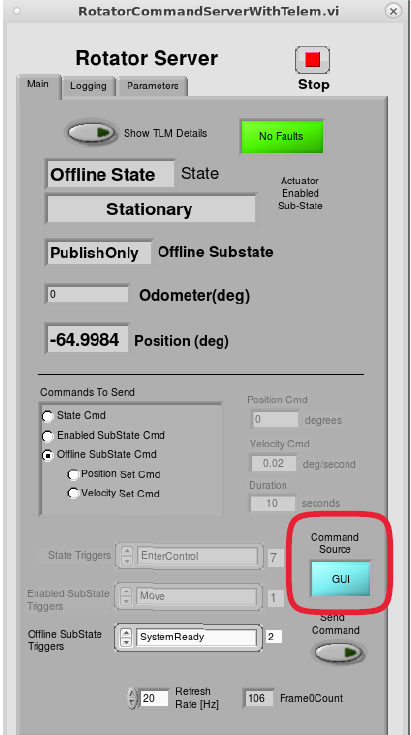
\includegraphics[width=1.79167in]{jira_imgs/1014.png}\\
If the Command Source does not show DDS, go to the Parameters tab,
select DDS under the Command Source and click the Set Command Source
button.\\
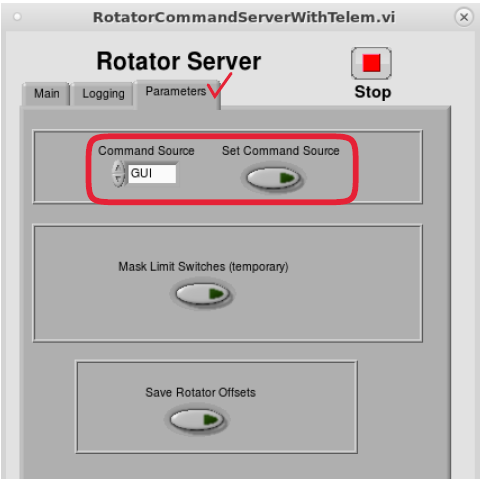
\includegraphics[width=1.79167in]{jira_imgs/1013.png}\textbf{Note:~If
the GUI is used after being set to DDS mode, the system will switch back
the Command Source to GUI and ignore any DDS commands. The Command
Source must show DDS in order to receive DDS commands.}

\medskip }
\end{minipage}
\\ \cdashline{2-2}


 & Expected Result \\
 & \begin{minipage}[t]{15cm}{\footnotesize
\smallskip
The system is capable of receiving/responding to DDS commands.

\medskip }
\end{minipage} \\ \cdashline{2-2}

 & Actual Result \\
 & \begin{minipage}[t]{15cm}{\footnotesize
\smallskip
When the command source was switched to DDS, we were able to command the
system remotely.

\medskip }
\end{minipage} \\ \cdashline{2-2}

 & Status: \textbf{ Initial Pass } \\ \hline

5 & Description \\
 & \begin{minipage}[t]{15cm}
{\footnotesize
\smallskip
\textbf{OFFLINESTATE -\textgreater{} STANDBYSTATE}\\
The system receives an \emph{enterControl State Transition} command
through DDS.

\medskip }
\end{minipage}
\\ \cdashline{2-2}


 & Expected Result \\
 & \begin{minipage}[t]{15cm}{\footnotesize
\smallskip
The system transitions into the StandbyState and is capable of
receiving/responding to DDS commands.\\
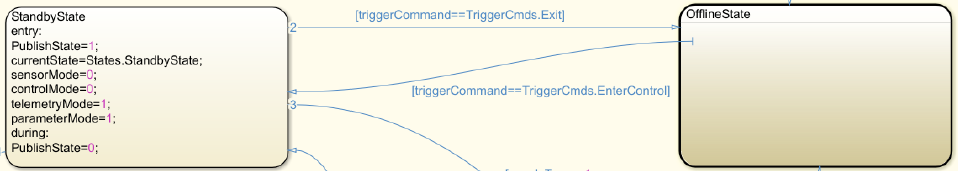
\includegraphics[width=4.68750in]{jira_imgs/1018.png}

\medskip }
\end{minipage} \\ \cdashline{2-2}

 & Actual Result \\
 & \begin{minipage}[t]{15cm}{\footnotesize
\smallskip
We were able to transition the system into the StandbyState through the
DDS.

\medskip }
\end{minipage} \\ \cdashline{2-2}

 & Status: \textbf{ Initial Pass } \\ \hline

6 & Description \\
 & \begin{minipage}[t]{15cm}
{\footnotesize
\smallskip
\textbf{STANDBYSTATE -\textgreater{} DISABLEDSTATE}\\
From the StandbyState, send a \emph{start} command through the DDS.

\medskip }
\end{minipage}
\\ \cdashline{2-2}


 & Expected Result \\
 & \begin{minipage}[t]{15cm}{\footnotesize
\smallskip
The system transitions into DisabledState after receiving/responding to
DDS command and the wrapper in the PXI real time controller looks for
the configuration file.\\
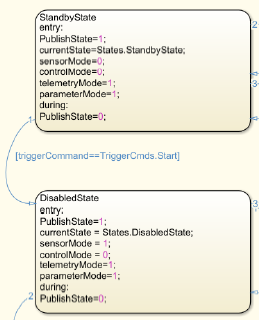
\includegraphics[width=1.79167in]{jira_imgs/1019.png}\\
If the configuration file is invalid or out of range, the system will
transition into a Fault State

\medskip }
\end{minipage} \\ \cdashline{2-2}

 & Actual Result \\
 & \begin{minipage}[t]{15cm}{\footnotesize
\smallskip
We were able to transition the system into the DisabledState through the
DDS.

\medskip }
\end{minipage} \\ \cdashline{2-2}

 & Status: \textbf{ Initial Pass } \\ \hline

7 & Description \\
 & \begin{minipage}[t]{15cm}
{\footnotesize
\smallskip
\textbf{DISABLEDSTATE -\textgreater{} ENABLEDSTATE}\\
From the DisabledState, send an \emph{enable state} command through the
DDS.

\medskip }
\end{minipage}
\\ \cdashline{2-2}


 & Expected Result \\
 & \begin{minipage}[t]{15cm}{\footnotesize
\smallskip
The system transitions into the EnabledState/Stationary substate, the
motor drives are enabled, motor brakes are released and the system is
capable of receiving/responding to DDS commands.\\
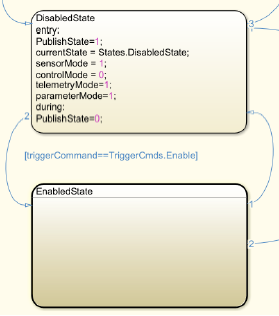
\includegraphics[width=1.79167in]{jira_imgs/1020.png}\\

\medskip }
\end{minipage} \\ \cdashline{2-2}

 & Actual Result \\
 & \begin{minipage}[t]{15cm}{\footnotesize
\smallskip
We were able to transition the system into the EnabledState using the
DDS and command movement to the Camera Rotator.

\medskip }
\end{minipage} \\ \cdashline{2-2}

 & Status: \textbf{ Initial Pass } \\ \hline

8 & Description \\
 & \begin{minipage}[t]{15cm}
{\footnotesize
\smallskip
\textbf{FAULTSTATE}\\
If a Fault occurs in any of the other states, the system will
automatically transition to the Fault State. While in the Fault state,
send a \emph{clearError} command through the DDS.\\
Note: If the fault that occurs goes through the interlock system, reset
the safety relay switch and send a \emph{clearError} command.

\medskip }
\end{minipage}
\\ \cdashline{2-2}


 & Expected Result \\
 & \begin{minipage}[t]{15cm}{\footnotesize
\smallskip
The system transitions back to the OfflineState/PublishOnly substate and
is not capable of receiving/responding to DDS commands. (Go back to Step
3)\\
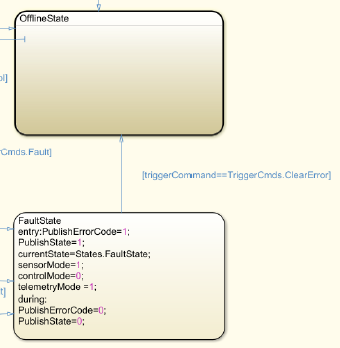
\includegraphics[width=1.79167in]{jira_imgs/1021.png}

\medskip }
\end{minipage} \\ \cdashline{2-2}

 & Actual Result \\
 & \begin{minipage}[t]{15cm}{\footnotesize
\smallskip
When the system experiened a ``SMLNK fault declared'', we were able to
use the \emph{clearError~}command through the DDS to bring it back to
Offline State.

\medskip }
\end{minipage} \\ \cdashline{2-2}

 & Status: \textbf{ Initial Pass } \\ \hline

9 & Description \\
 & \begin{minipage}[t]{15cm}
{\footnotesize
\smallskip
\textbf{GUI vs DDS Control}\\[2\baselineskip]While in DDS mode, send a
command from the EUI to test if an EUI user may take over control of the
camera rotator.

\medskip }
\end{minipage}
\\ \cdashline{2-2}


 & Expected Result \\
 & \begin{minipage}[t]{15cm}{\footnotesize
\smallskip
The system switches from DDS mode to GUI mode. The user must switch back
to the DDS Command Source through the GUI for the system to be
controlled through the CSC again.

\medskip }
\end{minipage} \\ \cdashline{2-2}

 & Actual Result \\
 & \begin{minipage}[t]{15cm}{\footnotesize
\smallskip

\medskip }
\end{minipage} \\ \cdashline{2-2}

 & Status: \textbf{ Initial Pass } \\ \hline

10 & Description \\
 & \begin{minipage}[t]{15cm}
{\footnotesize
\smallskip
\textbf{Back To DDS Mode}\\
While the system is in GUI mode, go to the Parameters tab, select DDS
under the Command Source and click the Set Command Source
button\textbf{.~}

\medskip }
\end{minipage}
\\ \cdashline{2-2}


 & Expected Result \\
 & \begin{minipage}[t]{15cm}{\footnotesize
\smallskip
The system is capable of receiving/responding to DDS commands.

\medskip }
\end{minipage} \\ \cdashline{2-2}

 & Actual Result \\
 & \begin{minipage}[t]{15cm}{\footnotesize
\smallskip
When the Command Source was switched to DDS, the system was able to
receive/respond to DDS commands.

\medskip }
\end{minipage} \\ \cdashline{2-2}

 & Status: \textbf{ Initial Pass } \\ \hline

11 & Description \\
 & \begin{minipage}[t]{15cm}
{\footnotesize
\smallskip
\textbf{Section 3.2.2 of the attached Software Acceptance Test
Procedure\\
Test Sequence \#1 -- PositionSet and Move Commands}\\[2\baselineskip]In
the Enabled/Stationary state, send a \emph{positionSet} command of 12
deg.

\medskip }
\end{minipage}
\\ \cdashline{2-2}


 & Expected Result \\
 & \begin{minipage}[t]{15cm}{\footnotesize
\smallskip
Confirm that the rotator does not move.

\medskip }
\end{minipage} \\ \cdashline{2-2}

 & Actual Result \\
 & \begin{minipage}[t]{15cm}{\footnotesize
\smallskip
The Camera Rotator did not move.

\medskip }
\end{minipage} \\ \cdashline{2-2}

 & Status: \textbf{ Initial Pass } \\ \hline

12 & Description \\
 & \begin{minipage}[t]{15cm}
{\footnotesize
\smallskip
Send a \emph{positionSet} command of 15deg.

\medskip }
\end{minipage}
\\ \cdashline{2-2}


 & Expected Result \\
 & \begin{minipage}[t]{15cm}{\footnotesize
\smallskip
Confirm that the rotator does not move.

\medskip }
\end{minipage} \\ \cdashline{2-2}

 & Actual Result \\
 & \begin{minipage}[t]{15cm}{\footnotesize
\smallskip
The Camera Rotator did not move.

\medskip }
\end{minipage} \\ \cdashline{2-2}

 & Status: \textbf{ Initial Pass } \\ \hline

13 & Description \\
 & \begin{minipage}[t]{15cm}
{\footnotesize
\smallskip
Send a \emph{move} command.\\[2\baselineskip]

\medskip }
\end{minipage}
\\ \cdashline{2-2}


 & Expected Result \\
 & \begin{minipage}[t]{15cm}{\footnotesize
\smallskip
Confirm that the rotator moves to 15deg and an \emph{inPosition} event
is generated when the move is complete.

\medskip }
\end{minipage} \\ \cdashline{2-2}

 & Actual Result \\
 & \begin{minipage}[t]{15cm}{\footnotesize
\smallskip
The Camera Rotator moved to 15 degrees and while the
\emph{inPosition~}event was published with the inPosition parameter set
to\emph{~}True, the \emph{inPosition~}event was published with the
inPosition parameter was immediately set to\emph{~False.}

\medskip }
\end{minipage} \\ \cdashline{2-2}

 & Issues found executing this step:  \\
 & \begin{minipage}[t]{13cm}{\footnotesize
\smallskip
\href{https://jira.lsstcorp.org/browse/LVV-18471}{LVV-18471}~~The inPosition parameter immediately publishes False after True

\medskip }
\end{minipage} \\ \cdashline{2-2}
 & Status: \textbf{ Initial Pass } \\ \hline

14 & Description \\
 & \begin{minipage}[t]{15cm}
{\footnotesize
\smallskip
Record the corresponding DDS events that were generated.

\medskip }
\end{minipage}
\\ \cdashline{2-2}


 & Expected Result \\
 & \begin{minipage}[t]{15cm}{\footnotesize
\smallskip
\begin{itemize}
\tightlist
\item
  The \emph{Application} event outputs reasonable values
\item
  The controllerState.enabledSubstate goes to MOVING\_POINT\_TO\_POINT
  when the move begins and STATIONARY when the move ends
\end{itemize}

\medskip }
\end{minipage} \\ \cdashline{2-2}

 & Actual Result \\
 & \begin{minipage}[t]{15cm}{\footnotesize
\smallskip
The GUI displayed MOVING\_POINT\_TO\_POINT while the Camera Rotator was
moving and displayed the STATIONARY state when the position reached 15
degrees.

\medskip }
\end{minipage} \\ \cdashline{2-2}

 & Status: \textbf{ Initial Pass } \\ \hline

15 & Description \\
 & \begin{minipage}[t]{15cm}
{\footnotesize
\smallskip
\textbf{Section 3.2.2 of the attached Software Acceptance Test
Procedure\\
Test Sequence \#2 - Stop Command}\\[2\baselineskip]In the
Enabled/Stationary state, send a \emph{positionSet} command of 50 deg.

\medskip }
\end{minipage}
\\ \cdashline{2-2}


 & Expected Result \\
 & \begin{minipage}[t]{15cm}{\footnotesize
\smallskip
Confirm that the rotator does not move.

\medskip }
\end{minipage} \\ \cdashline{2-2}

 & Actual Result \\
 & \begin{minipage}[t]{15cm}{\footnotesize
\smallskip
The Camera Rotator did not move.

\medskip }
\end{minipage} \\ \cdashline{2-2}

 & Status: \textbf{ Initial Pass } \\ \hline

16 & Description \\
 & \begin{minipage}[t]{15cm}
{\footnotesize
\smallskip
Send a \emph{move} command.

\medskip }
\end{minipage}
\\ \cdashline{2-2}


 & Expected Result \\
 & \begin{minipage}[t]{15cm}{\footnotesize
\smallskip
The rotator starts its rotation.

\medskip }
\end{minipage} \\ \cdashline{2-2}

 & Actual Result \\
 & \begin{minipage}[t]{15cm}{\footnotesize
\smallskip
The Camera Rotator began is movement to 50degrees.

\medskip }
\end{minipage} \\ \cdashline{2-2}

 & Status: \textbf{ Initial Pass } \\ \hline

17 & Description \\
 & \begin{minipage}[t]{15cm}
{\footnotesize
\smallskip
While the rotator is still moving, send a \emph{Stop} command.

\medskip }
\end{minipage}
\\ \cdashline{2-2}


 & Expected Result \\
 & \begin{minipage}[t]{15cm}{\footnotesize
\smallskip
Confirm that the system quickly comes to a stop before reaching the 50
deg position.

\medskip }
\end{minipage} \\ \cdashline{2-2}

 & Actual Result \\
 & \begin{minipage}[t]{15cm}{\footnotesize
\smallskip
The Camera Rotator stopped at 33 degrees.

\medskip }
\end{minipage} \\ \cdashline{2-2}

 & Status: \textbf{ Initial Pass } \\ \hline

18 & Description \\
 & \begin{minipage}[t]{15cm}
{\footnotesize
\smallskip
Send a \emph{positionSet} command of 60 deg followed by a \emph{move}
command.

\medskip }
\end{minipage}
\\ \cdashline{2-2}


 & Expected Result \\
 & \begin{minipage}[t]{15cm}{\footnotesize
\smallskip
Confirm the rotator moves to the commanded position following the
previous stop command.

\medskip }
\end{minipage} \\ \cdashline{2-2}

 & Actual Result \\
 & \begin{minipage}[t]{15cm}{\footnotesize
\smallskip
The Camera Rotator moved to 60 degrees after being stopped at 33
degrees.

\medskip }
\end{minipage} \\ \cdashline{2-2}

 & Status: \textbf{ Initial Pass } \\ \hline

19 & Description \\
 & \begin{minipage}[t]{15cm}
{\footnotesize
\smallskip
Record the corresponding DDS events that were generated.

\medskip }
\end{minipage}
\\ \cdashline{2-2}


 & Expected Result \\
 & \begin{minipage}[t]{15cm}{\footnotesize
\smallskip
\begin{itemize}
\tightlist
\item
  The controllerState.enabledSubstate goes to CONTROLLED\_STOPPING when
  the stop is requested, then STATIONARY when the rotator has halted
\item
  The \emph{inPosition} event is not reported as True.
\end{itemize}

\medskip }
\end{minipage} \\ \cdashline{2-2}

 & Actual Result \\
 & \begin{minipage}[t]{15cm}{\footnotesize
\smallskip
The substate changed to CONTROLLED\_STOPPING when the \emph{stop} was
requested but still moving and then STATIONARY when the rotator was
stopped.

\medskip }
\end{minipage} \\ \cdashline{2-2}

 & Status: \textbf{ Initial Pass } \\ \hline

20 & Description \\
 & \begin{minipage}[t]{15cm}
{\footnotesize
\smallskip
\textbf{Test of trackStart and track command}\\[2\baselineskip]In the
Enabled state, send a \emph{trackStart} command. Do not send a
\emph{Track} command.

\medskip }
\end{minipage}
\\ \cdashline{2-2}


 & Expected Result \\
 & \begin{minipage}[t]{15cm}{\footnotesize
\smallskip
The cRIO goes into FAULT state without moving at all.

\medskip }
\end{minipage} \\ \cdashline{2-2}

 & Actual Result \\
 & \begin{minipage}[t]{15cm}{\footnotesize
\smallskip
12/9- The Camera Rotator did not FAULT, still moved to 10 degrees and
continued to slowly move toward 0 degrees without a \emph{Track~}command
being sent.\\[2\baselineskip]12/10- Our assumption is that whatever the
\emph{trackStart} command is, the cRio begins to calculate the
trajectory of the track and does not FAULT when a \emph{Track} command
is not sent. Instead, when a new \emph{trackStart~}command is sent, the
cRio continues to calculate the trajectory from the previous command.

\medskip }
\end{minipage} \\ \cdashline{2-2}

 & Issues found executing this step:  \\
 & \begin{minipage}[t]{13cm}{\footnotesize
\smallskip
\href{https://jira.lsstcorp.org/browse/LVV-18474}{LVV-18474}~~System does not fault when sent a trackStart without a track command

\medskip }
\end{minipage} \\ \cdashline{2-2}
 & Status: \textbf{ Fail } \\ \hline

21 & Description \\
 & \begin{minipage}[t]{15cm}
{\footnotesize
\smallskip
\textbf{Section 3.2.2 of the attached Software Acceptance Test
Procedure\\
Test Sequence \#4 - Track and TrackStart Commands}\\[2\baselineskip]In
the Enabled/Stationary state, send a \emph{trackStart} command.

\medskip }
\end{minipage}
\\ \cdashline{2-2}


 & Expected Result \\
 & \begin{minipage}[t]{15cm}{\footnotesize
\smallskip
Confirm that the system transitions into Enabled/Slewing and Tracking
state.

\medskip }
\end{minipage} \\ \cdashline{2-2}

 & Actual Result \\
 & \begin{minipage}[t]{15cm}{\footnotesize
\smallskip
The system was seen to transition into the SlewAndTracking substate of
the Enabled state.

\medskip }
\end{minipage} \\ \cdashline{2-2}

 & Status: \textbf{ Initial Pass } \\ \hline

22 & Description \\
 & \begin{minipage}[t]{15cm}
{\footnotesize
\smallskip
Send a series of \emph{track} commands at 20 Hz from
command\_vector\_set\_A.mat and ensure the system follows the commands
and sends appropriate tracking and trackLost events.

\medskip }
\end{minipage}
\\ \cdashline{2-2}

 & Test Data \\
 & \begin{minipage}[t]{15cm}{\footnotesize
\smallskip
\textbf{Deviation:} When the \emph{trackStart} command is run, a track
command must be issued at 10-20Hz until tracking is done. The vendor's
code reads in a CSV file with tracking conditions when using the
\emph{trackStart} command in order to circumvent a FAULT state due to
lack of position, velocity and time updates. Instead, use Russell's code
which utilizes the functions \emph{ramp~}and\emph{~sine~}to track from a
start position to an end position at a specified velocity and track
along a sine wave, respectively.

\medskip }
\end{minipage} \\ \cdashline{2-2}

 & Expected Result \\
 & \begin{minipage}[t]{15cm}{\footnotesize
\smallskip
The rotator first slews to meet the commanded path and then tracks that
path

\medskip }
\end{minipage} \\ \cdashline{2-2}

 & Actual Result \\
 & \begin{minipage}[t]{15cm}{\footnotesize
\smallskip
12/9 - The Camera Rotator continued to track toward +10degrees from the
previous command and was then commanded to track to -2000degrees which
set off the negative software limit when the Camera Rotator reached
-90degrees.

\medskip }
\end{minipage} \\ \cdashline{2-2}

 & Issues found executing this step:  \\
 & \begin{minipage}[t]{13cm}{\footnotesize
\smallskip
\href{https://jira.lsstcorp.org/browse/LVV-18474}{LVV-18474}~~System does not fault when sent a trackStart without a track command

\medskip }
\end{minipage} \\ \cdashline{2-2}
 & Status: \textbf{ Fail } \\ \hline

23 & Description \\
 & \begin{minipage}[t]{15cm}
{\footnotesize
\smallskip
Record the corresponding DDS events that were generated.

\medskip }
\end{minipage}
\\ \cdashline{2-2}


 & Expected Result \\
 & \begin{minipage}[t]{15cm}{\footnotesize
\smallskip
\begin{itemize}
\tightlist
\item
  The \emph{Application~}event outputs reasonable values
\item
  The controllerState.enabledSubstate goes to SLEWING\_OR\_TRACKING when
  the move begins, CONTROLLED\_STOPPING when the movement sequence ends,
  and STATIONARY when the rotator has stopped
\item
  The \emph{inPosition} event is True once slewing has finished and
  tracking begins
\end{itemize}

\medskip }
\end{minipage} \\ \cdashline{2-2}

 & Actual Result \\
 & \begin{minipage}[t]{15cm}{\footnotesize
\smallskip
12/9 - The Camera Rotator was put into a FAULT state as the negative
software limit was tripped

\medskip }
\end{minipage} \\ \cdashline{2-2}

 & Issues found executing this step:  \\
 & \begin{minipage}[t]{13cm}{\footnotesize
\smallskip
\href{https://jira.lsstcorp.org/browse/LVV-18474}{LVV-18474}~~System does not fault when sent a trackStart without a track command

\medskip }
\end{minipage} \\ \cdashline{2-2}
 & Status: \textbf{ Fail } \\ \hline

24 & Description \\
 & \begin{minipage}[t]{15cm}
{\footnotesize
\smallskip
\textbf{Section 3.2.2 of the attached Software Acceptance Test
Procedure\\
Test Sequence \#5 - Track and TrackStart Commands}\\[2\baselineskip]In
the Enabled/Stationary state, send a \emph{trackStart} command.

\medskip }
\end{minipage}
\\ \cdashline{2-2}


 & Expected Result \\
 & \begin{minipage}[t]{15cm}{\footnotesize
\smallskip
Confirm that the system transitions into Enabled/Slewing and Tracking
state.

\medskip }
\end{minipage} \\ \cdashline{2-2}

 & Actual Result \\
 & \begin{minipage}[t]{15cm}{\footnotesize
\smallskip
The pointing component was used to command the Camera Rotator to track.
The system correctly transitioned into the Enabled/SlewingAndTracking
state.

\medskip }
\end{minipage} \\ \cdashline{2-2}

 & Status: \textbf{ Initial Pass } \\ \hline

25 & Description \\
 & \begin{minipage}[t]{15cm}
{\footnotesize
\smallskip
Send a series of \emph{track} commands at 20 Hz from
command\_vector\_set\_B.mat and ensure the system follows the commands
and sends appropriate tracking and trackLost events.

\medskip }
\end{minipage}
\\ \cdashline{2-2}

 & Test Data \\
 & \begin{minipage}[t]{15cm}{\footnotesize
\smallskip
\textbf{Deviation:} When the \emph{trackStart} command is run, a track
command must be issued at 10-20Hz until tracking is done. The vendor's
code reads in a CSV file with tracking conditions when using the
\emph{trackStart} command in order to circumvent a FAULT state due to
lack of position, velocity and time updates. Instead, use Russell's code
which utilizes the functions \emph{ramp~}and\emph{~sine~}to track from a
start position to an end position at a specified velocity and track
along a sine wave, respectively.

\medskip }
\end{minipage} \\ \cdashline{2-2}

 & Expected Result \\
 & \begin{minipage}[t]{15cm}{\footnotesize
\smallskip
The rotator first slews to meet the commanded path and then tracks that
path

\medskip }
\end{minipage} \\ \cdashline{2-2}

 & Actual Result \\
 & \begin{minipage}[t]{15cm}{\footnotesize
\smallskip
The Camera Rotator first moved to -60degrees and continued
TrackingAndSlewing for 30 seconds before moving back to the
Enabled/Stationary state.

\medskip }
\end{minipage} \\ \cdashline{2-2}

 & Status: \textbf{ Initial Pass } \\ \hline

26 & Description \\
 & \begin{minipage}[t]{15cm}
{\footnotesize
\smallskip
Record the corresponding DDS events that were generated.

\medskip }
\end{minipage}
\\ \cdashline{2-2}


 & Expected Result \\
 & \begin{minipage}[t]{15cm}{\footnotesize
\smallskip
\begin{itemize}
\tightlist
\item
  The \emph{Application~}event outputs reasonable values
\item
  The controllerState.enabledSubstate goes to SLEWING\_OR\_TRACKING when
  the move begins, CONTROLLED\_STOPPING when the movement sequence ends,
  and STATIONARY when the rotator has stopped
\item
  The \emph{inPosition} event is True once slewing has finished and
  tracking begins
\end{itemize}

\medskip }
\end{minipage} \\ \cdashline{2-2}

 & Actual Result \\
 & \begin{minipage}[t]{15cm}{\footnotesize
\smallskip
The Camera Rotator correctly entered the SlewingAndTracking when moving
and Stationary when the move ended.

\medskip }
\end{minipage} \\ \cdashline{2-2}

 & Status: \textbf{ Initial Pass } \\ \hline

27 & Description \\
 & \begin{minipage}[t]{15cm}
{\footnotesize
\smallskip
\textbf{Section 3.2.2 of the attached Software Acceptance Test
Procedure\\
Test Sequence \#6 - configureVelocity Command}\\[2\baselineskip]In the
Enabled/Stationary state, send a \emph{configureVelocity} command of 4
deg/s.

\medskip }
\end{minipage}
\\ \cdashline{2-2}


 & Expected Result \\
 & \begin{minipage}[t]{15cm}{\footnotesize
\smallskip
Confirm that the command is rejected for being out of acceptable range.

\medskip }
\end{minipage} \\ \cdashline{2-2}

 & Actual Result \\
 & \begin{minipage}[t]{15cm}{\footnotesize
\smallskip
The velocity was out of acceptable range and caused the DDS command to
fail.

\medskip }
\end{minipage} \\ \cdashline{2-2}

 & Status: \textbf{ Initial Pass } \\ \hline

28 & Description \\
 & \begin{minipage}[t]{15cm}
{\footnotesize
\smallskip
Send a \emph{configureVelocity} command of 0.5 deg/s.

\medskip }
\end{minipage}
\\ \cdashline{2-2}


 & Expected Result \\
 & \begin{minipage}[t]{15cm}{\footnotesize
\smallskip
Confirm that this command is accepted.

\medskip }
\end{minipage} \\ \cdashline{2-2}

 & Actual Result \\
 & \begin{minipage}[t]{15cm}{\footnotesize
\smallskip
The velocity was accepted.

\medskip }
\end{minipage} \\ \cdashline{2-2}

 & Status: \textbf{ Initial Pass } \\ \hline

29 & Description \\
 & \begin{minipage}[t]{15cm}
{\footnotesize
\smallskip
Send a \emph{positionSet} command to a position 10 deg away from the
current position. Send a \emph{move} command.

\medskip }
\end{minipage}
\\ \cdashline{2-2}


 & Expected Result \\
 & \begin{minipage}[t]{15cm}{\footnotesize
\smallskip
Confirm the that move in completed in approximately 20 seconds.

\medskip }
\end{minipage} \\ \cdashline{2-2}

 & Actual Result \\
 & \begin{minipage}[t]{15cm}{\footnotesize
\smallskip
The move was timed and took approximately 20 seconds to move 10degrees.

\medskip }
\end{minipage} \\ \cdashline{2-2}

 & Status: \textbf{ Initial Pass } \\ \hline

30 & Description \\
 & \begin{minipage}[t]{15cm}
{\footnotesize
\smallskip
Record the corresponding DDS events that were generated.

\medskip }
\end{minipage}
\\ \cdashline{2-2}


 & Expected Result \\
 & \begin{minipage}[t]{15cm}{\footnotesize
\smallskip
\begin{itemize}
\tightlist
\item
  The \emph{Application} event outputs reasonable values
\item
  The controllerState.enabledSubstate goes to MOVING\_POINT\_TO\_POINT
  when the move begins and STATIONARY when the move ends
\item
  The \emph{inPosition} event is True once move has finished
\end{itemize}

\medskip }
\end{minipage} \\ \cdashline{2-2}

 & Actual Result \\
 & \begin{minipage}[t]{15cm}{\footnotesize
\smallskip
The GUI showed that the system was in Enabled/MovingPt2Pt when moving
and Stationary when the move ended.~

\medskip }
\end{minipage} \\ \cdashline{2-2}

 & Status: \textbf{ Initial Pass } \\ \hline

31 & Description \\
 & \begin{minipage}[t]{15cm}
{\footnotesize
\smallskip
\textbf{Section 3.2.2 of the attached Software Acceptance Test
Procedure\\
Test Sequence \#7 - configureAcceleration Command}\\[2\baselineskip]In
the Enabled/Stationary state with the \emph{configureVelocity} command
from the previous test still in effect, send a
\emph{configureAcceleration} command of 2 deg/s\^{}2.

\medskip }
\end{minipage}
\\ \cdashline{2-2}


 & Expected Result \\
 & \begin{minipage}[t]{15cm}{\footnotesize
\smallskip
Confirm that the command is rejected for being out of acceptable range.

\medskip }
\end{minipage} \\ \cdashline{2-2}

 & Actual Result \\
 & \begin{minipage}[t]{15cm}{\footnotesize
\smallskip
The acceleration was out of acceptable range and caused the DDS command
to fail.

\medskip }
\end{minipage} \\ \cdashline{2-2}

 & Status: \textbf{ Initial Pass } \\ \hline

32 & Description \\
 & \begin{minipage}[t]{15cm}
{\footnotesize
\smallskip
Send a \emph{configureAcceleration} command of 0.05 deg/s\^{}2.

\medskip }
\end{minipage}
\\ \cdashline{2-2}


 & Expected Result \\
 & \begin{minipage}[t]{15cm}{\footnotesize
\smallskip
Confirm that the command is accepted.

\medskip }
\end{minipage} \\ \cdashline{2-2}

 & Actual Result \\
 & \begin{minipage}[t]{15cm}{\footnotesize
\smallskip
The acceleration was accepted.

\medskip }
\end{minipage} \\ \cdashline{2-2}

 & Status: \textbf{ Initial Pass } \\ \hline

33 & Description \\
 & \begin{minipage}[t]{15cm}
{\footnotesize
\smallskip
Send a \emph{positionSet} command to a position 10 deg away from the
current position. Send a \emph{move} command.

\medskip }
\end{minipage}
\\ \cdashline{2-2}


 & Expected Result \\
 & \begin{minipage}[t]{15cm}{\footnotesize
\smallskip
Confirm the that move in completed in approximately 30 seconds.

\medskip }
\end{minipage} \\ \cdashline{2-2}

 & Actual Result \\
 & \begin{minipage}[t]{15cm}{\footnotesize
\smallskip
The move was timed and took approximately 30 seconds to move 10 degrees.

\medskip }
\end{minipage} \\ \cdashline{2-2}

 & Status: \textbf{ Initial Pass } \\ \hline

34 & Description \\
 & \begin{minipage}[t]{15cm}
{\footnotesize
\smallskip
Record the corresponding DDS events that were generated.

\medskip }
\end{minipage}
\\ \cdashline{2-2}


 & Expected Result \\
 & \begin{minipage}[t]{15cm}{\footnotesize
\smallskip
\begin{itemize}
\tightlist
\item
  The \emph{Application} event outputs reasonable values
\item
  The controllerState.enabledSubstate goes to MOVING\_POINT\_TO\_POINT
  when the move begins and STATIONARY when the move ends
\item
  The \emph{inPosition} event is True once move has finished
\end{itemize}

\medskip }
\end{minipage} \\ \cdashline{2-2}

 & Actual Result \\
 & \begin{minipage}[t]{15cm}{\footnotesize
\smallskip
The GUI showed that the system was in Enabled/MovingPt2Pt when moving
and Stationary when the move ended.

\medskip }
\end{minipage} \\ \cdashline{2-2}

 & Status: \textbf{ Initial Pass } \\ \hline

35 & Description \\
 & \begin{minipage}[t]{15cm}
{\footnotesize
\smallskip
Shutdown the rotator.

\medskip }
\end{minipage}
\\ \cdashline{2-2}


 & Expected Result \\
 & \begin{minipage}[t]{15cm}{\footnotesize
\smallskip
Rotator is shutdown.

\medskip }
\end{minipage} \\ \cdashline{2-2}

 & Actual Result \\
 & \begin{minipage}[t]{15cm}{\footnotesize
\smallskip
The Camera Rotator was shutdown every night by hitting the E-stop,
verifying this step.

\medskip }
\end{minipage} \\ \cdashline{2-2}

 & Status: \textbf{ Initial Pass } \\ \hline

36 & Description \\
 & \begin{minipage}[t]{15cm}
{\footnotesize
\smallskip
\textbf{Section 3.3.2 of the attached Software Acceptance Test
Procedure}\\
\textbf{Rotator Action on State Commands\\
}\\
Start up the system.

\medskip }
\end{minipage}
\\ \cdashline{2-2}


 & Expected Result \\
 & \begin{minipage}[t]{15cm}{\footnotesize
\smallskip
\begin{itemize}
\tightlist
\item
  Confirm the system starts up in Offline/PublishOnly state.
\item
  When the middleware starts up, confirm that a \emph{SettingsVersions}
  event is published with a list of all saved settings file names and a
  \emph{settingsApplied} event is published with a list of all default
  configurable parameters.
\end{itemize}

\medskip }
\end{minipage} \\ \cdashline{2-2}

 & Actual Result \\
 & \begin{minipage}[t]{15cm}{\footnotesize
\smallskip
The Camera Rotator was started up every morning after being shut down
from the previous night.~

\medskip }
\end{minipage} \\ \cdashline{2-2}

 & Status: \textbf{ Initial Pass } \\ \hline

37 & Description \\
 & \begin{minipage}[t]{15cm}
{\footnotesize
\smallskip
Send the \emph{enterControl} command.

\medskip }
\end{minipage}
\\ \cdashline{2-2}


 & Expected Result \\
 & \begin{minipage}[t]{15cm}{\footnotesize
\smallskip
Confirm that the system does not respond to a \emph{EnterControl}
command over DDS.

\medskip }
\end{minipage} \\ \cdashline{2-2}

 & Actual Result \\
 & \begin{minipage}[t]{15cm}{\footnotesize
\smallskip
The system prompted an error stating ``Controller has CSC command
disabled, use the EUI to enable CSC commands''

\medskip }
\end{minipage} \\ \cdashline{2-2}

 & Status: \textbf{ Initial Pass } \\ \hline

38 & Description \\
 & \begin{minipage}[t]{15cm}
{\footnotesize
\smallskip
From the EUI send an offline substate trigger of \emph{systemReady}.

\medskip }
\end{minipage}
\\ \cdashline{2-2}


 & Expected Result \\
 & \begin{minipage}[t]{15cm}{\footnotesize
\smallskip
Confirm system goes into Offline/Available substate.

\medskip }
\end{minipage} \\ \cdashline{2-2}

 & Actual Result \\
 & \begin{minipage}[t]{15cm}{\footnotesize
\smallskip
The system was seen to transition to the Offline/Available substate when
a~\emph{systemReady}~command was sent from the EUI only.

\medskip }
\end{minipage} \\ \cdashline{2-2}

 & Status: \textbf{ Initial Pass } \\ \hline

39 & Description \\
 & \begin{minipage}[t]{15cm}
{\footnotesize
\smallskip
From the EUI, select the DDS button to allow the system to receive
commands from DDS.

\medskip }
\end{minipage}
\\ \cdashline{2-2}


 & Expected Result \\
 & \begin{minipage}[t]{15cm}{\footnotesize
\smallskip
The EUI displays you are in DDS command mode.

\medskip }
\end{minipage} \\ \cdashline{2-2}

 & Actual Result \\
 & \begin{minipage}[t]{15cm}{\footnotesize
\smallskip
The command source confirmed that the system was in DDS command mode.

\medskip }
\end{minipage} \\ \cdashline{2-2}

 & Status: \textbf{ Initial Pass } \\ \hline

40 & Description \\
 & \begin{minipage}[t]{15cm}
{\footnotesize
\smallskip
Send an \emph{EnterControl} trigger. Record the corresponding DDS
event(s) that were generated.

\medskip }
\end{minipage}
\\ \cdashline{2-2}


 & Expected Result \\
 & \begin{minipage}[t]{15cm}{\footnotesize
\smallskip
Confirm the system transitions from Offline/Available to Standby state.

\medskip }
\end{minipage} \\ \cdashline{2-2}

 & Actual Result \\
 & \begin{minipage}[t]{15cm}{\footnotesize
\smallskip
The system correctly transitions from the Offline/Available state to the
Standby state.

\medskip }
\end{minipage} \\ \cdashline{2-2}

 & Status: \textbf{ Initial Pass } \\ \hline

41 & Description \\
 & \begin{minipage}[t]{15cm}
{\footnotesize
\smallskip
Send a \emph{Start} trigger with an invalid filename.

\medskip }
\end{minipage}
\\ \cdashline{2-2}


 & Expected Result \\
 & \begin{minipage}[t]{15cm}{\footnotesize
\smallskip
Verify that the command is rejected and the system does not transition
out of Standby state.

\medskip }
\end{minipage} \\ \cdashline{2-2}

 & Actual Result \\
 & \begin{minipage}[t]{15cm}{\footnotesize
\smallskip
With Russell's code, we cannot test this because Russell has all the
default parameters hardcoded so it doesn't look for a config file.

\medskip }
\end{minipage} \\ \cdashline{2-2}

 & Status: \textbf{ Not Executed } \\ \hline

42 & Description \\
 & \begin{minipage}[t]{15cm}
{\footnotesize
\smallskip
Send a \emph{Start} trigger with a valid filename. Record the
corresponding DDS event(s) that were generated.

\medskip }
\end{minipage}
\\ \cdashline{2-2}


 & Expected Result \\
 & \begin{minipage}[t]{15cm}{\footnotesize
\smallskip
Confirm the system transitions from Standby to Disabled state and a
\emph{settingApplied} and \emph{AppliedSettingsMatchStart} = True events
are generated.

\medskip }
\end{minipage} \\ \cdashline{2-2}

 & Actual Result \\
 & \begin{minipage}[t]{15cm}{\footnotesize
\smallskip
With Russell's code, we cannot test this because Russell has all the
default parameters hardcoded so it doesn't look for a config file.

\medskip }
\end{minipage} \\ \cdashline{2-2}

 & Status: \textbf{ Not Executed } \\ \hline

43 & Description \\
 & \begin{minipage}[t]{15cm}
{\footnotesize
\smallskip
Send an \emph{Enable} trigger. Record the corresponding DDS event(s)
that were generated.

\medskip }
\end{minipage}
\\ \cdashline{2-2}


 & Expected Result \\
 & \begin{minipage}[t]{15cm}{\footnotesize
\smallskip
Confirm the system transitions from Disabled to Enabled state.

\medskip }
\end{minipage} \\ \cdashline{2-2}

 & Actual Result \\
 & \begin{minipage}[t]{15cm}{\footnotesize
\smallskip
The system correctly transitioned from the Disabled state to the Enabled
state following the~\emph{Enable} command.

\medskip }
\end{minipage} \\ \cdashline{2-2}

 & Status: \textbf{ Initial Pass } \\ \hline

44 & Description \\
 & \begin{minipage}[t]{15cm}
{\footnotesize
\smallskip
Send a \emph{Disable} trigger. Record the corresponding DDS event(s)
that were generated.

\medskip }
\end{minipage}
\\ \cdashline{2-2}


 & Expected Result \\
 & \begin{minipage}[t]{15cm}{\footnotesize
\smallskip
Confirm the system transitions from Enabled to Disabled state.

\medskip }
\end{minipage} \\ \cdashline{2-2}

 & Actual Result \\
 & \begin{minipage}[t]{15cm}{\footnotesize
\smallskip
The system correctly transitioned from the Enabled state to the Disabled
state following the~\emph{Disable} command.

\medskip }
\end{minipage} \\ \cdashline{2-2}

 & Status: \textbf{ Initial Pass } \\ \hline

45 & Description \\
 & \begin{minipage}[t]{15cm}
{\footnotesize
\smallskip
Send a \emph{Standby} trigger. Record the corresponding DDS event(s)
that were generated.

\medskip }
\end{minipage}
\\ \cdashline{2-2}


 & Expected Result \\
 & \begin{minipage}[t]{15cm}{\footnotesize
\smallskip
Confirm the system transitions from Disabled state to Standby state.

\medskip }
\end{minipage} \\ \cdashline{2-2}

 & Actual Result \\
 & \begin{minipage}[t]{15cm}{\footnotesize
\smallskip
The system correctly transitioned from the Disabled state to the Standby
state following the~\emph{Standby}~command.

\medskip }
\end{minipage} \\ \cdashline{2-2}

 & Status: \textbf{ Initial Pass } \\ \hline

46 & Description \\
 & \begin{minipage}[t]{15cm}
{\footnotesize
\smallskip
Send a \emph{exitControl} trigger. Record the corresponding DDS event(s)
that were generated.

\medskip }
\end{minipage}
\\ \cdashline{2-2}


 & Expected Result \\
 & \begin{minipage}[t]{15cm}{\footnotesize
\smallskip
Confirm the system transitions from Standby state to Offline state.

\medskip }
\end{minipage} \\ \cdashline{2-2}

 & Actual Result \\
 & \begin{minipage}[t]{15cm}{\footnotesize
\smallskip
The system correctly transitioned from the Standby state to the Offline
state following the~\emph{exitControl}~command.~

\medskip }
\end{minipage} \\ \cdashline{2-2}

 & Status: \textbf{ Initial Pass } \\ \hline

47 & Description \\
 & \begin{minipage}[t]{15cm}
{\footnotesize
\smallskip
\textbf{Section 5.1 of the attached Software Acceptance Test
Procedure}\\
\textbf{Rotator Events\\
}\\
In the Enabled state, unplug an encoder cable for one of the rotator
motors.

\medskip }
\end{minipage}
\\ \cdashline{2-2}

 & Test Data \\
 & \begin{minipage}[t]{15cm}{\footnotesize
\smallskip
\textbf{NOTE:} After each step in this set of steps, we will need to
send the clearError command to the CSC. This will put the cRIO into
Offline/PublishOnly. Use the EUI to re-enable CSC control.

\medskip }
\end{minipage} \\ \cdashline{2-2}

 & Expected Result \\
 & \begin{minipage}[t]{15cm}{\footnotesize
\smallskip
Confirm that a \emph{Drive Fault} event is created and the system
transitions to Fault state.

\medskip }
\end{minipage} \\ \cdashline{2-2}

 & Actual Result \\
 & \begin{minipage}[t]{15cm}{\footnotesize
\smallskip
We did not test this because we would need to pull up the schematics for
the wiring of the camera rotator motors in order to ensure we were
pulling the correct cables.

\medskip }
\end{minipage} \\ \cdashline{2-2}

 & Status: \textbf{ Not Executed } \\ \hline

48 & Description \\
 & \begin{minipage}[t]{15cm}
{\footnotesize
\smallskip
In the Enabled state, unplug a linear encoder cable for the rotator.

\medskip }
\end{minipage}
\\ \cdashline{2-2}


 & Expected Result \\
 & \begin{minipage}[t]{15cm}{\footnotesize
\smallskip
Confirm that a \emph{Linear Encoder Error} event is created and the
system transitions to Fault state.

\medskip }
\end{minipage} \\ \cdashline{2-2}

 & Actual Result \\
 & \begin{minipage}[t]{15cm}{\footnotesize
\smallskip
We did not test this because we would need to pull up the schematics for
the wiring of the camera rotator motors in order to ensure we were
pulling the correct cables.

\medskip }
\end{minipage} \\ \cdashline{2-2}

 & Status: \textbf{ Not Executed } \\ \hline

49 & Description \\
 & \begin{minipage}[t]{15cm}
{\footnotesize
\smallskip
Set the Following Error Threshold parameter to a very small value
(0.0001 deg or smaller) and command a \emph{PositionSet/Move}.

\medskip }
\end{minipage}
\\ \cdashline{2-2}


 & Expected Result \\
 & \begin{minipage}[t]{15cm}{\footnotesize
\smallskip
Confirm that a \emph{Following Error} event is created and the system
transitions to Fault state.

\medskip }
\end{minipage} \\ \cdashline{2-2}

 & Actual Result \\
 & \begin{minipage}[t]{15cm}{\footnotesize
\smallskip
With Russell's code, we cannot test this because his code does not
acknowledge the changed Following Error Threshold parameter (from 0.1 to
0.0001 degrees) in the default file.

\medskip }
\end{minipage} \\ \cdashline{2-2}

 & Status: \textbf{ Not Executed } \\ \hline

50 & Description \\
 & \begin{minipage}[t]{15cm}
{\footnotesize
\smallskip
Activate the positive software limit using a special control program.

\medskip }
\end{minipage}
\\ \cdashline{2-2}


 & Expected Result \\
 & \begin{minipage}[t]{15cm}{\footnotesize
\smallskip
Confirm that a \emph{Positive Limit Switch} error message is created and
the system transitions to Fault state.

\medskip }
\end{minipage} \\ \cdashline{2-2}

 & Actual Result \\
 & \begin{minipage}[t]{15cm}{\footnotesize
\smallskip
Due to Russell's code, we could not change the positive software limit
from +90 degrees so we verified that a track command of +95 degrees was
rejected.

\medskip }
\end{minipage} \\ \cdashline{2-2}

 & Status: \textbf{ Initial Pass } \\ \hline

51 & Description \\
 & \begin{minipage}[t]{15cm}
{\footnotesize
\smallskip
Activate the negative software limit using a special control program.

\medskip }
\end{minipage}
\\ \cdashline{2-2}


 & Expected Result \\
 & \begin{minipage}[t]{15cm}{\footnotesize
\smallskip
Confirm that a \emph{Negative Limit Switch} error message is created and
the system transitions to Fault State.

\medskip }
\end{minipage} \\ \cdashline{2-2}

 & Actual Result \\
 & \begin{minipage}[t]{15cm}{\footnotesize
\smallskip
12/9 - The Negative Limit Switch was tripped at -90.6083degrees and the
system was transitioned to a FAULT state as a result of the testing of
the track command (Step 22).\\
Note: This functionality is in the software but was not executed. The
assumption is that because the calculations were being done internally
within the simulink model, the commanded track position was not checked
to be within the acceptable range.\\[2\baselineskip]12/11 - Due to
Russell's code, we could not change the negative software limit from -90
degrees so we verified that a track command of -95 degrees was rejected.

\medskip }
\end{minipage} \\ \cdashline{2-2}

 & Status: \textbf{ Initial Pass } \\ \hline

52 & Description \\
 & \begin{minipage}[t]{15cm}
{\footnotesize
\smallskip
Unplug the Ethercat cable between the control PC and the Copley XE2
drive.

\medskip }
\end{minipage}
\\ \cdashline{2-2}


 & Expected Result \\
 & \begin{minipage}[t]{15cm}{\footnotesize
\smallskip
Confirm that an \emph{Ethercat Problem} event is created and the system
transitions to Fault state.

\medskip }
\end{minipage} \\ \cdashline{2-2}

 & Actual Result \\
 & \begin{minipage}[t]{15cm}{\footnotesize
\smallskip
We did not test this because we would need to pull up the schematics for
the wiring of the camera rotator motors in order to ensure we were
pulling the correct cables.

\medskip }
\end{minipage} \\ \cdashline{2-2}

 & Status: \textbf{ Not Executed } \\ \hline

53 & Description \\
 & \begin{minipage}[t]{15cm}
{\footnotesize
\smallskip
Shutdown the rotator.

\medskip }
\end{minipage}
\\ \cdashline{2-2}


 & Expected Result \\
 & \begin{minipage}[t]{15cm}{\footnotesize
\smallskip
Rotator is shutdown.

\medskip }
\end{minipage} \\ \cdashline{2-2}

 & Actual Result \\
 & \begin{minipage}[t]{15cm}{\footnotesize
\smallskip
As previously stated, the Camera Rotator is shut down every night
through the E-stop.

\medskip }
\end{minipage} \\ \cdashline{2-2}

 & Status: \textbf{ Initial Pass } \\ \hline

\end{longtable}

\paragraph{Test Case LVV-T1569 - Integrated CCW + HR Interlock Test
 }\mbox{}\\

Open  \href{https://jira.lsstcorp.org/secure/Tests.jspa#/testCase/LVV-T1569}{\textit{ LVV-T1569 } }
test case in Jira.

The objective of this test case is to verify the interlocks of the
integrated CCW and Camera Rotator. This test case will exercise the
functionality of the combined interlock system between the CCW and the
Camera Rotator and meets the following criteria:

\begin{itemize}
\tightlist
\item
  Requires CCW AUX IS to be connected to the Camera Rotator IS
\item
  Requires WOBBLE assembly to be electrically and mechanically connected
\item
  Does \textbf{NOT} require the camera rotator to be loaded with the
  camera simulated mass or actual camera hardware
\item
  Does \textbf{NOT~}require CCW and Camera Rotator to be under combined
  control
\end{itemize}

The interlock system requirements for the Camera Rotator were previously
verified during the software functional re-verification test at the
summit facility. The test procedure used during the re-verification
testing is the \emph{LSST Hexapods-Rotator Software Acceptance Test
Procedure} which is attached to this test case. This includes the
procedure that covered how the interlocks were triggered for the Camera
Rotator, however it is a different configuration with the CCW
integrated.


\textbf{ Preconditions}:\\
Prior to the execution of this test case to verify the interlocks of the
CCW + HR, the following Summit tasks must be completed:\\

\begin{itemize}
\tightlist
\item
  The CCW has been installed on the Camera Cart

  \begin{itemize}
  \tightlist
  \item
    \url{https://jira.lsstcorp.org/browse/SUMMIT-2156}
  \end{itemize}
\item
  The functional testing of the Camera Rotator Hardware~

  \begin{itemize}
  \tightlist
  \item
    h\href{https://jira.lsstcorp.org/browse/SUMMIT-3370}{ttps://jira.lsstcorp.org/browse/SUMMIT-3370}
  \end{itemize}
\item
  The functional testing of the Camera Rotator Software without SAL

  \begin{itemize}
  \tightlist
  \item
    \url{https://jira.lsstcorp.org/browse/SUMMIT-3371}
  \end{itemize}
\item
  The Camera rotator has been connected to the electronics cabinets and
  the connections have been tested

  \begin{itemize}
  \tightlist
  \item
    \url{https://jira.lsstcorp.org/browse/SUMMIT-3294}
  \end{itemize}
\item
  The Hexapod and Rotator have been installed on camera cart

  \begin{itemize}
  \tightlist
  \item
    \url{https://jira.lsstcorp.org/browse/SUMMIT-3224}
  \end{itemize}
\item
  The cables and cabinets have been checked

  \begin{itemize}
  \tightlist
  \item
    \url{https://jira.lsstcorp.org/browse/SUMMIT-3231}
  \end{itemize}
\end{itemize}


Execution status: {\bf Fail }

Final comment:\\


Detailed steps results:

\begin{longtable}{p{1cm}p{15cm}}
\hline
{Step} & Step Details\\ \hline
1 & Description \\
 & \begin{minipage}[t]{15cm}
{\footnotesize
\smallskip
\textbf{STARTING THE EUI}\\[2\baselineskip]Double click the Hexapod GUI
Viewer desktop icon on the computer.

\begin{itemize}
\tightlist
\item
  This can be done on the Dell Management PC or another computer on the
  same network
\end{itemize}

\medskip }
\end{minipage}
\\ \cdashline{2-2}


 & Expected Result \\
 & \begin{minipage}[t]{15cm}{\footnotesize
\smallskip
A prompt to enter a password is shown.~

\medskip }
\end{minipage} \\ \cdashline{2-2}

 & Actual Result \\
 & \begin{minipage}[t]{15cm}{\footnotesize
\smallskip
This was previously verified in the \emph{Integration of Camera Rotator
with SAL 4.0 (LSST)} Test Case.

\medskip }
\end{minipage} \\ \cdashline{2-2}

 & Status: \textbf{ Initial Pass } \\ \hline

2 & Description \\
 & \begin{minipage}[t]{15cm}
{\footnotesize
\smallskip
Enter the password ``lsst-vnc''

\begin{itemize}
\tightlist
\item
  If the EUI isn't automatically up and running when the VNC opens,
  double click on the CAM\_Hex\_eGUI or M2\_Hex\_eGUI icon on the VNC
  viewer
\end{itemize}

\medskip }
\end{minipage}
\\ \cdashline{2-2}


 & Expected Result \\
 & \begin{minipage}[t]{15cm}{\footnotesize
\smallskip
The EUI is in the Offline State/PublishOnly substate and is able to
publish through SAL but cannot receive commands.

\medskip }
\end{minipage} \\ \cdashline{2-2}

 & Actual Result \\
 & \begin{minipage}[t]{15cm}{\footnotesize
\smallskip
This was previously verified in the\emph{~Integration of Camera Rotator
with SAL 4.0 (LSST)~}Test Case.

\medskip }
\end{minipage} \\ \cdashline{2-2}

 & Status: \textbf{ Initial Pass } \\ \hline

3 & Description \\
 & \begin{minipage}[t]{15cm}
{\footnotesize
\smallskip
\textbf{OFFLINESTATE/AVAILABLESTATE}\\
On the Main tab, select the ``Offline SubState Cmd'' field in the
Commands to Send section, set the Offline SubState Triggers to ``System
Ready'' and click on the Send Command button.\\
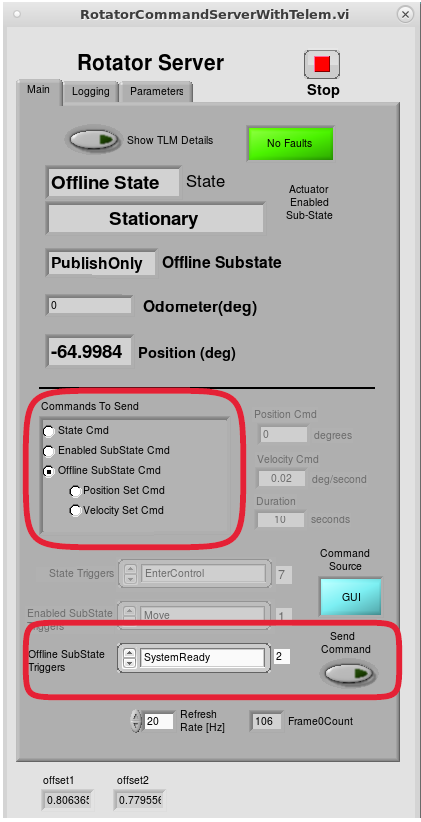
\includegraphics[width=1.79167in]{jira_imgs/1005.png}

\medskip }
\end{minipage}
\\ \cdashline{2-2}


 & Expected Result \\
 & \begin{minipage}[t]{15cm}{\footnotesize
\smallskip
The system transitions from the OfflineState/PublishOnly substate to the
OfflineState/AvailableState
substate.\\[2\baselineskip]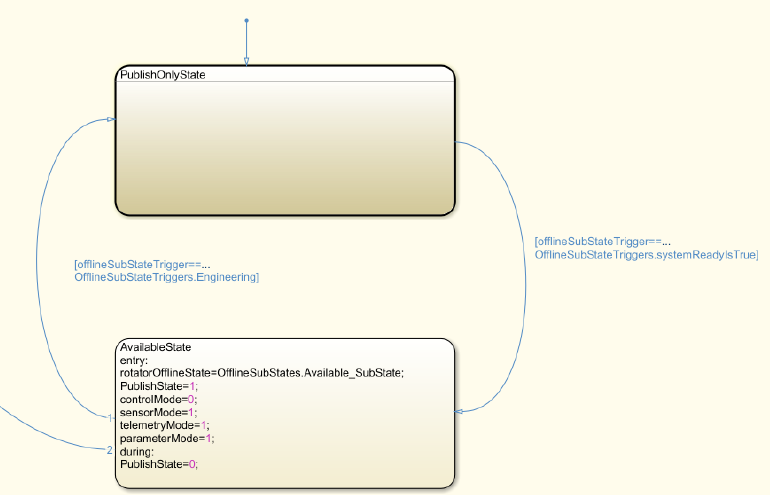
\includegraphics[width=1.79167in]{jira_imgs/1007.png}

\medskip }
\end{minipage} \\ \cdashline{2-2}

 & Actual Result \\
 & \begin{minipage}[t]{15cm}{\footnotesize
\smallskip
This was previously verified in the\emph{~Integration of Camera Rotator
with SAL 4.0 (LSST)~}Test Case.

\medskip }
\end{minipage} \\ \cdashline{2-2}

 & Status: \textbf{ Initial Pass } \\ \hline

4 & Description \\
 & \begin{minipage}[t]{15cm}
{\footnotesize
\smallskip
\textbf{SWITCHING TO DDS MODE}\\
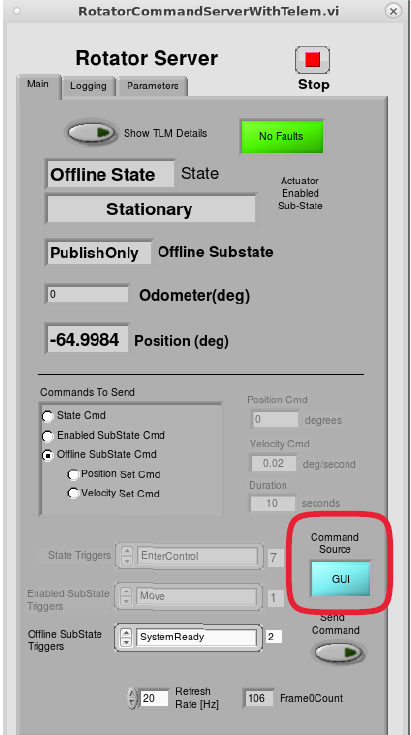
\includegraphics[width=1.79167in]{jira_imgs/1014.png}\\
If the Command Source does not show DDS, go to the Parameters tab,
select DDS under the Command Source and click the Set Command Source
button.\\
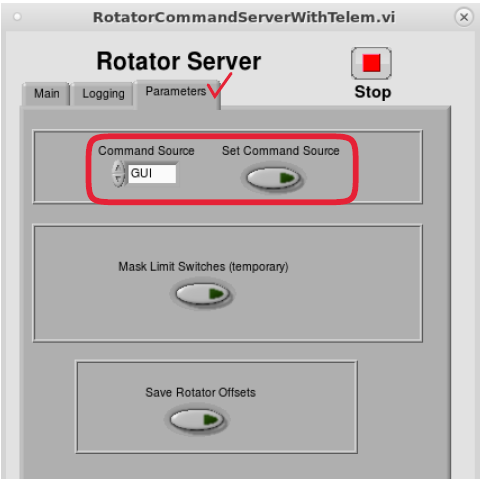
\includegraphics[width=1.79167in]{jira_imgs/1013.png}\textbf{Note:~If
the GUI is used after being set to DDS mode, the system will switch back
the Command Source to GUI and ignore any DDS commands. The Command
Source must show DDS in order to receive DDS commands.}

\medskip }
\end{minipage}
\\ \cdashline{2-2}


 & Expected Result \\
 & \begin{minipage}[t]{15cm}{\footnotesize
\smallskip
The system is capable of receiving/responding to DDS commands.

\medskip }
\end{minipage} \\ \cdashline{2-2}

 & Actual Result \\
 & \begin{minipage}[t]{15cm}{\footnotesize
\smallskip
This was previously verified in the\emph{~Integration of Camera Rotator
with SAL 4.0 (LSST)~}Test Case.

\medskip }
\end{minipage} \\ \cdashline{2-2}

 & Status: \textbf{ Initial Pass } \\ \hline

5 & Description \\
 & \begin{minipage}[t]{15cm}
{\footnotesize
\smallskip
\textbf{OFFLINESTATE -\textgreater{} STANDBYSTATE}\\
The system receives an \emph{enterControl State Transition} command
through DDS.

\medskip }
\end{minipage}
\\ \cdashline{2-2}


 & Expected Result \\
 & \begin{minipage}[t]{15cm}{\footnotesize
\smallskip
The system transitions into the StandbyState and is capable of
receiving/responding to DDS commands.\\
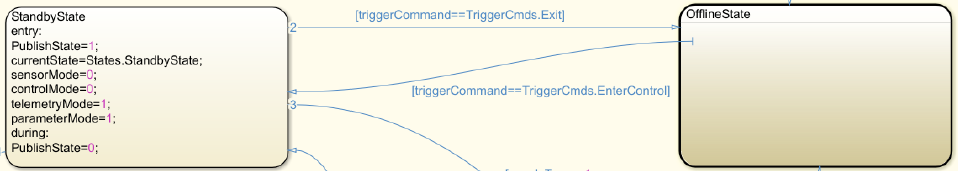
\includegraphics[width=4.68750in]{jira_imgs/1018.png}

\medskip }
\end{minipage} \\ \cdashline{2-2}

 & Actual Result \\
 & \begin{minipage}[t]{15cm}{\footnotesize
\smallskip
This was previously verified in the\emph{~Integration of Camera Rotator
with SAL 4.0 (LSST)~}Test Case.

\medskip }
\end{minipage} \\ \cdashline{2-2}

 & Status: \textbf{ Initial Pass } \\ \hline

6 & Description \\
 & \begin{minipage}[t]{15cm}
{\footnotesize
\smallskip
\textbf{STANDBYSTATE -\textgreater{} DISABLEDSTATE}\\
From the StandbyState, send a \emph{start} command through the DDS.

\medskip }
\end{minipage}
\\ \cdashline{2-2}


 & Expected Result \\
 & \begin{minipage}[t]{15cm}{\footnotesize
\smallskip
The system transitions into DisabledState after receiving/responding to
DDS command and the wrapper in the PXI real time controller looks for
the configuration file.\\
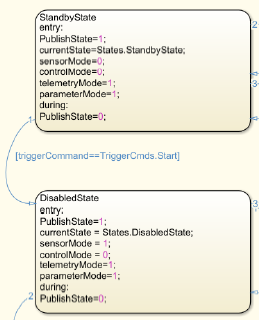
\includegraphics[width=1.79167in]{jira_imgs/1019.png}\\
If the configuration file is invalid or out of range, the system will
transition into a Fault State

\medskip }
\end{minipage} \\ \cdashline{2-2}

 & Actual Result \\
 & \begin{minipage}[t]{15cm}{\footnotesize
\smallskip
This was previously verified in the\emph{~Integration of Camera Rotator
with SAL 4.0 (LSST)~}Test Case.

\medskip }
\end{minipage} \\ \cdashline{2-2}

 & Status: \textbf{ Initial Pass } \\ \hline

7 & Description \\
 & \begin{minipage}[t]{15cm}
{\footnotesize
\smallskip
\textbf{DISABLEDSTATE -\textgreater{} ENABLEDSTATE}\\
From the DisabledState, send an \emph{enable state} command through the
DDS.

\medskip }
\end{minipage}
\\ \cdashline{2-2}


 & Expected Result \\
 & \begin{minipage}[t]{15cm}{\footnotesize
\smallskip
The system transitions into the EnabledState/Stationary substate, the
motor drives are enabled, motor brakes are released and the system is
capable of receiving/responding to DDS commands.\\
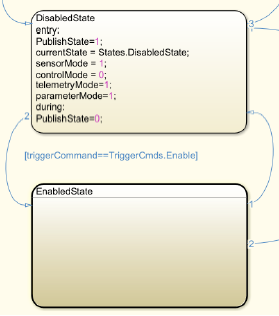
\includegraphics[width=1.79167in]{jira_imgs/1020.png}\\

\medskip }
\end{minipage} \\ \cdashline{2-2}

 & Actual Result \\
 & \begin{minipage}[t]{15cm}{\footnotesize
\smallskip
This was previously verified in the\emph{~Integration of Camera Rotator
with SAL 4.0 (LSST)~}Test Case.

\medskip }
\end{minipage} \\ \cdashline{2-2}

 & Status: \textbf{ Initial Pass } \\ \hline

8 & Description \\
 & \begin{minipage}[t]{15cm}
{\footnotesize
\smallskip
\textbf{FAULTSTATE}\\
If a Fault occurs in any of the other states, the system will
automatically transition to the Fault State. While in the Fault state,
send a \emph{clearError} command through the DDS.\\
Note: If the fault that occurs goes through the interlock system, reset
the safety relay switch and send a \emph{clearError} command.

\medskip }
\end{minipage}
\\ \cdashline{2-2}


 & Expected Result \\
 & \begin{minipage}[t]{15cm}{\footnotesize
\smallskip
The system transitions back to the OfflineState/PublishOnly substate and
is not capable of receiving/responding to DDS commands. (Go back to Step
3)\\
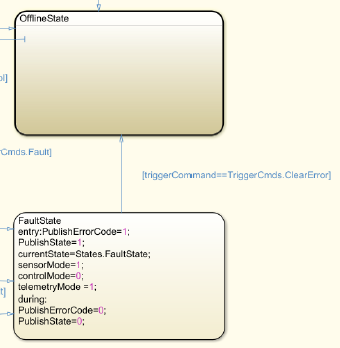
\includegraphics[width=1.79167in]{jira_imgs/1021.png}

\medskip }
\end{minipage} \\ \cdashline{2-2}

 & Actual Result \\
 & \begin{minipage}[t]{15cm}{\footnotesize
\smallskip
This was previously verified in the\emph{~Integration of Camera Rotator
with SAL 4.0 (LSST)~}Test Case.

\medskip }
\end{minipage} \\ \cdashline{2-2}

 & Status: \textbf{ Initial Pass } \\ \hline

9 & Description \\
 & \begin{minipage}[t]{15cm}
{\footnotesize
\smallskip
Start up the CCW such that it is in the Enabled state.
\textbf{{(Tekniker)}}

\medskip }
\end{minipage}
\\ \cdashline{2-2}


 & Expected Result \\
 & \begin{minipage}[t]{15cm}{\footnotesize
\smallskip
The CCW is in the Enabled State.

\medskip }
\end{minipage} \\ \cdashline{2-2}

 & Actual Result \\
 & \begin{minipage}[t]{15cm}{\footnotesize
\smallskip
Tekniker transitioned the CCW into the Enabled State through the CCW
GUI.

\medskip }
\end{minipage} \\ \cdashline{2-2}

 & Status: \textbf{ Initial Pass } \\ \hline

10 & Description \\
 & \begin{minipage}[t]{15cm}
{\footnotesize
\smallskip
\textbf{Camera Rotator Interlock}\\[2\baselineskip]With the CCW and the
Camera Rotator in the Enabled state, but \textbf{NOT} moving, Press the
E-Stop which is wired in series with the fully retracted limit switches
to simulate the limit switches.\\
{\\
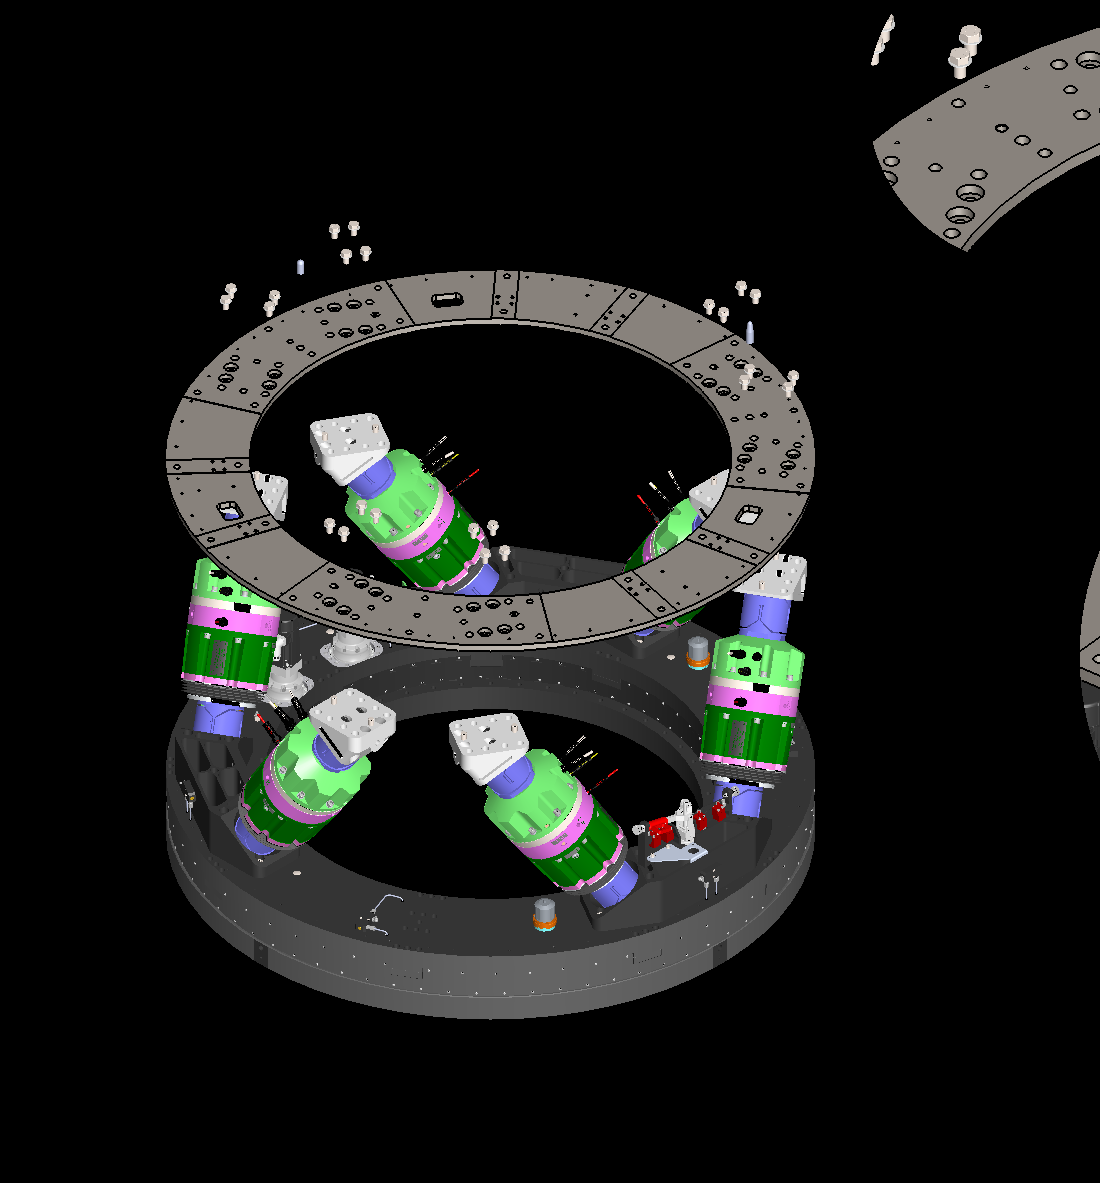
\includegraphics[width=3.12500in]{jira_imgs/998.png}}\\
{\\
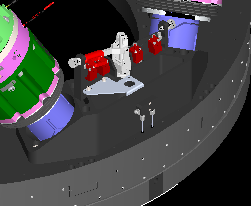
\includegraphics[width=3.12500in]{jira_imgs/999.png}}

\medskip }
\end{minipage}
\\ \cdashline{2-2}


 & Expected Result \\
 & \begin{minipage}[t]{15cm}{\footnotesize
\smallskip
The fault within the Camera Rotator Interlock System disables the Camera
Rotator and CCW drives by a Safe Torque Off trigger.

\medskip }
\end{minipage} \\ \cdashline{2-2}

 & Actual Result \\
 & \begin{minipage}[t]{15cm}{\footnotesize
\smallskip
This was test by hitting the Camera Rotator E-Stop and was verified to
fault both the CCW and Camera Rotator Interlock System.

\medskip }
\end{minipage} \\ \cdashline{2-2}

 & Status: \textbf{ Initial Pass } \\ \hline

11 & Description \\
 & \begin{minipage}[t]{15cm}
{\footnotesize
\smallskip
Manually reset the interlock system by cycling the safety reset switch.

\medskip }
\end{minipage}
\\ \cdashline{2-2}


 & Expected Result \\
 & \begin{minipage}[t]{15cm}{\footnotesize
\smallskip
The safety interlock fault has been cleared in the PILZ controller.

\medskip }
\end{minipage} \\ \cdashline{2-2}

 & Actual Result \\
 & \begin{minipage}[t]{15cm}{\footnotesize
\smallskip
The safety switch was reset by simultaneously twisting and pulling up
the E-Stop button to its original position.

\medskip }
\end{minipage} \\ \cdashline{2-2}

 & Status: \textbf{ Initial Pass } \\ \hline

12 & Description \\
 & \begin{minipage}[t]{15cm}
{\footnotesize
\smallskip
Transition out of the fault state by sending a \emph{ClearError}
trigger.

\medskip }
\end{minipage}
\\ \cdashline{2-2}


 & Expected Result \\
 & \begin{minipage}[t]{15cm}{\footnotesize
\smallskip
The system transitions from the Fault state to the Offline/PublishOnly
State.

\medskip }
\end{minipage} \\ \cdashline{2-2}

 & Actual Result \\
 & \begin{minipage}[t]{15cm}{\footnotesize
\smallskip
The~\emph{ClearError~}command was sent through both the Camera Rotator
and CCW GUI in order to transition each out of the Fault state.

\medskip }
\end{minipage} \\ \cdashline{2-2}

 & Status: \textbf{ Initial Pass } \\ \hline

13 & Description \\
 & \begin{minipage}[t]{15cm}
{\footnotesize
\smallskip
Bring the CCW and the Camera Rotator back to the Enabled state.

\medskip }
\end{minipage}
\\ \cdashline{2-2}


 & Expected Result \\
 & \begin{minipage}[t]{15cm}{\footnotesize
\smallskip
CCW and Camera Rotator are in the Enabled state.

\medskip }
\end{minipage} \\ \cdashline{2-2}

 & Actual Result \\
 & \begin{minipage}[t]{15cm}{\footnotesize
\smallskip
The CCW and Camera Rotator were commanded through their respective GUI's
to transition back to the Enabled State.

\medskip }
\end{minipage} \\ \cdashline{2-2}

 & Status: \textbf{ Initial Pass } \\ \hline

14 & Description \\
 & \begin{minipage}[t]{15cm}
{\footnotesize
\smallskip
\textbf{CCW Interlock}\\[2\baselineskip]With the CCW and the Camera
Rotator in the Enabled state, but \textbf{NOT} moving, Press the E-Stop
which is wired in series with the fully retracted limit switches to
simulate the limit switches.

\medskip }
\end{minipage}
\\ \cdashline{2-2}


 & Expected Result \\
 & \begin{minipage}[t]{15cm}{\footnotesize
\smallskip
The fault within the CCW Interlock System disables the Camera Rotator
and CCW drives by a Safe Torque Off trigger.

\medskip }
\end{minipage} \\ \cdashline{2-2}

 & Actual Result \\
 & \begin{minipage}[t]{15cm}{\footnotesize
\smallskip
This was test by hitting the CCW E-Stop and was verified to fault both
the CCW and Camera Rotator Interlock System.

\medskip }
\end{minipage} \\ \cdashline{2-2}

 & Status: \textbf{ Initial Pass } \\ \hline

15 & Description \\
 & \begin{minipage}[t]{15cm}
{\footnotesize
\smallskip
Manually reset the interlock system by cycling the safety reset switch.

\medskip }
\end{minipage}
\\ \cdashline{2-2}


 & Expected Result \\
 & \begin{minipage}[t]{15cm}{\footnotesize
\smallskip
The safety interlock fault has been cleared in the PILZ controller.

\medskip }
\end{minipage} \\ \cdashline{2-2}

 & Actual Result \\
 & \begin{minipage}[t]{15cm}{\footnotesize
\smallskip
The safety switch was reset by simultaneously twisting and pulling up
the E-Stop button to its original position.

\medskip }
\end{minipage} \\ \cdashline{2-2}

 & Status: \textbf{ Initial Pass } \\ \hline

16 & Description \\
 & \begin{minipage}[t]{15cm}
{\footnotesize
\smallskip
Transition out of the fault state by sending a~\emph{ClearError}
trigger\emph{.}

\medskip }
\end{minipage}
\\ \cdashline{2-2}


 & Expected Result \\
 & \begin{minipage}[t]{15cm}{\footnotesize
\smallskip
The system transitions from the Fault state to the Offline/PublishOnly
State.

\medskip }
\end{minipage} \\ \cdashline{2-2}

 & Actual Result \\
 & \begin{minipage}[t]{15cm}{\footnotesize
\smallskip
The system successfully transitioned out the of the Fault state by
sending a \emph{ClearError} after the interlock was reset.

\medskip }
\end{minipage} \\ \cdashline{2-2}

 & Status: \textbf{ Initial Pass } \\ \hline

17 & Description \\
 & \begin{minipage}[t]{15cm}
{\footnotesize
\smallskip
Bring the CCW and the Camera Rotator back to the Enabled state.

\medskip }
\end{minipage}
\\ \cdashline{2-2}


 & Expected Result \\
 & \begin{minipage}[t]{15cm}{\footnotesize
\smallskip
CCW and Camera Rotator are in the Enabled state.

\medskip }
\end{minipage} \\ \cdashline{2-2}

 & Actual Result \\
 & \begin{minipage}[t]{15cm}{\footnotesize
\smallskip
The CCW and Camera Rotator were commanded through their respective GUI's
to transition back to the Enabled State.

\medskip }
\end{minipage} \\ \cdashline{2-2}

 & Status: \textbf{ Initial Pass } \\ \hline

18 & Description \\
 & \begin{minipage}[t]{15cm}
{\footnotesize
\smallskip
{\textbf{Manual Test of the CCW Interlock}\\[2\baselineskip]Remove the
locking pin from the bar connecting the CCW and the Camera Rotator.}

\medskip }
\end{minipage}
\\ \cdashline{2-2}


 & Expected Result \\
 & \begin{minipage}[t]{15cm}{\footnotesize
\smallskip
{The CCW is able to move independently. }

\medskip }
\end{minipage} \\ \cdashline{2-2}

 & Actual Result \\
 & \begin{minipage}[t]{15cm}{\footnotesize
\smallskip

\medskip }
\end{minipage} \\ \cdashline{2-2}

 & Status: \textbf{ Not Executed } \\ \hline

19 & Description \\
 & \begin{minipage}[t]{15cm}
{\footnotesize
\smallskip
{Manually twist the bar connected to the CCW in the positive direction
until the positive limit switch is tripped.}

\medskip }
\end{minipage}
\\ \cdashline{2-2}


 & Expected Result \\
 & \begin{minipage}[t]{15cm}{\footnotesize
\smallskip
{The fault triggered on the CCW positive limit switch disables drives
for both the CCW and the Camera Rotator by a Safe Torque Off trigger.}

\medskip }
\end{minipage} \\ \cdashline{2-2}

 & Actual Result \\
 & \begin{minipage}[t]{15cm}{\footnotesize
\smallskip

\medskip }
\end{minipage} \\ \cdashline{2-2}

 & Status: \textbf{ Not Executed } \\ \hline

20 & Description \\
 & \begin{minipage}[t]{15cm}
{\footnotesize
\smallskip
Rotate the bar so that it is approximately at 0 degrees.

\medskip }
\end{minipage}
\\ \cdashline{2-2}


 & Expected Result \\
 & \begin{minipage}[t]{15cm}{\footnotesize
\smallskip
The CCW is midway between the limit switches.

\medskip }
\end{minipage} \\ \cdashline{2-2}

 & Actual Result \\
 & \begin{minipage}[t]{15cm}{\footnotesize
\smallskip

\medskip }
\end{minipage} \\ \cdashline{2-2}

 & Status: \textbf{ Not Executed } \\ \hline

21 & Description \\
 & \begin{minipage}[t]{15cm}
{\footnotesize
\smallskip
{Reset the interlock for the CCW (Tekniker) and Camera Rotator (see step
1.8 above)}

\medskip }
\end{minipage}
\\ \cdashline{2-2}


 & Expected Result \\
 & \begin{minipage}[t]{15cm}{\footnotesize
\smallskip
{The CCW and Camera Rotator are in the Enabled State.}

\medskip }
\end{minipage} \\ \cdashline{2-2}

 & Actual Result \\
 & \begin{minipage}[t]{15cm}{\footnotesize
\smallskip

\medskip }
\end{minipage} \\ \cdashline{2-2}

 & Status: \textbf{ Not Executed } \\ \hline

22 & Description \\
 & \begin{minipage}[t]{15cm}
{\footnotesize
\smallskip
{Manually twist the bar connected to the CCW in the negative direction
until the interlock is tripped.}

\medskip }
\end{minipage}
\\ \cdashline{2-2}


 & Expected Result \\
 & \begin{minipage}[t]{15cm}{\footnotesize
\smallskip
{The fault triggered on the CCW negative limit switch disables the
drives on the CCW by a Safe Torque Off Trigger.\\
}

\medskip }
\end{minipage} \\ \cdashline{2-2}

 & Actual Result \\
 & \begin{minipage}[t]{15cm}{\footnotesize
\smallskip

\medskip }
\end{minipage} \\ \cdashline{2-2}

 & Status: \textbf{ Not Executed } \\ \hline

23 & Description \\
 & \begin{minipage}[t]{15cm}
{\footnotesize
\smallskip
Rotate the bar so that it is approximately at 0 degrees.

\medskip }
\end{minipage}
\\ \cdashline{2-2}


 & Expected Result \\
 & \begin{minipage}[t]{15cm}{\footnotesize
\smallskip
The CCW is midway between the limit switches.

\medskip }
\end{minipage} \\ \cdashline{2-2}

 & Actual Result \\
 & \begin{minipage}[t]{15cm}{\footnotesize
\smallskip

\medskip }
\end{minipage} \\ \cdashline{2-2}

 & Status: \textbf{ Not Executed } \\ \hline

24 & Description \\
 & \begin{minipage}[t]{15cm}
{\footnotesize
\smallskip
Reset the interlock for the CCW (Tekniker) and Camera Rotator (see step
1.8 above)

\medskip }
\end{minipage}
\\ \cdashline{2-2}


 & Expected Result \\
 & \begin{minipage}[t]{15cm}{\footnotesize
\smallskip
The CCW and Camera Rotator are in the Enabled State.

\medskip }
\end{minipage} \\ \cdashline{2-2}

 & Actual Result \\
 & \begin{minipage}[t]{15cm}{\footnotesize
\smallskip

\medskip }
\end{minipage} \\ \cdashline{2-2}

 & Status: \textbf{ Not Executed } \\ \hline

25 & Description \\
 & \begin{minipage}[t]{15cm}
{\footnotesize
\smallskip
\textbf{{Pointing Component - Basic Control}}\\
{Insert the locking pin that so that the CCW moves synchronously to the
Camera Rotator.}

\medskip }
\end{minipage}
\\ \cdashline{2-2}


 & Expected Result \\
 & \begin{minipage}[t]{15cm}{\footnotesize
\smallskip
The CCW and Camera Rotator move synchronously to each other.

\medskip }
\end{minipage} \\ \cdashline{2-2}

 & Actual Result \\
 & \begin{minipage}[t]{15cm}{\footnotesize
\smallskip
The locking pin for the temporary linkage between the CCW and the Camera
Rotator remained inserted.

\medskip }
\end{minipage} \\ \cdashline{2-2}

 & Status: \textbf{ Initial Pass } \\ \hline

26 & Description \\
 & \begin{minipage}[t]{15cm}
{\footnotesize
\smallskip
The following steps define what the Jupyter Notebook for this test case
implements. Executing the Jupyter notebook is the only actual step that
needs to be executed.

\medskip }
\end{minipage}
\\ \cdashline{2-2}


 & Expected Result \\
 & \begin{minipage}[t]{15cm}{\footnotesize
\smallskip
The Jupyter notebook controls the system to run through the steps below.

\medskip }
\end{minipage} \\ \cdashline{2-2}

 & Actual Result \\
 & \begin{minipage}[t]{15cm}{\footnotesize
\smallskip
The Jupyter notebook was run successfully and allowed control of the
system

\medskip }
\end{minipage} \\ \cdashline{2-2}

 & Status: \textbf{ Initial Pass } \\ \hline

27 & Description \\
 & \begin{minipage}[t]{15cm}
{\footnotesize
\smallskip
Bring the Camera Rotator and the Pointing Component to the Enabled
State.

\medskip }
\end{minipage}
\\ \cdashline{2-2}


 & Expected Result \\
 & \begin{minipage}[t]{15cm}{\footnotesize
\smallskip
The Camera Rotator and Pointing Component are in the Enabled State.

\medskip }
\end{minipage} \\ \cdashline{2-2}

 & Actual Result \\
 & \begin{minipage}[t]{15cm}{\footnotesize
\smallskip
The Camera Rotator and Pointing Component were seen to be in the Enabled
State through the EFD.

\medskip }
\end{minipage} \\ \cdashline{2-2}

 & Status: \textbf{ Initial Pass } \\ \hline

28 & Description \\
 & \begin{minipage}[t]{15cm}
{\footnotesize
\smallskip
Send a \emph{trackStart} command to the rotator.~

\medskip }
\end{minipage}
\\ \cdashline{2-2}


 & Expected Result \\
 & \begin{minipage}[t]{15cm}{\footnotesize
\smallskip
The Camera Rotator transitions from the Enabled/Stationary state to the
Enabled/SlewingAndTracking state.

\medskip }
\end{minipage} \\ \cdashline{2-2}

 & Actual Result \\
 & \begin{minipage}[t]{15cm}{\footnotesize
\smallskip
The Camera Rotator successfully transitioned into the SlewingAndTracking
state as seen on the GUI.

\medskip }
\end{minipage} \\ \cdashline{2-2}

 & Status: \textbf{ Initial Pass } \\ \hline

29 & Description \\
 & \begin{minipage}[t]{15cm}
{\footnotesize
\smallskip
Send a \emph{track} command via the pointing component to track.

\medskip }
\end{minipage}
\\ \cdashline{2-2}


 & Expected Result \\
 & \begin{minipage}[t]{15cm}{\footnotesize
\smallskip
The Camera Rotator begins to track for 30 seconds.~

\medskip }
\end{minipage} \\ \cdashline{2-2}

 & Actual Result \\
 & \begin{minipage}[t]{15cm}{\footnotesize
\smallskip
The Camera Rotator and CCW began to move synchronously.

\medskip }
\end{minipage} \\ \cdashline{2-2}

 & Status: \textbf{ Initial Pass } \\ \hline

30 & Description \\
 & \begin{minipage}[t]{15cm}
{\footnotesize
\smallskip
Send a \emph{stopTracking} command to the pointing component

\medskip }
\end{minipage}
\\ \cdashline{2-2}


 & Expected Result \\
 & \begin{minipage}[t]{15cm}{\footnotesize
\smallskip
The pointing component stops sending \emph{track} commands.

\medskip }
\end{minipage} \\ \cdashline{2-2}

 & Actual Result \\
 & \begin{minipage}[t]{15cm}{\footnotesize
\smallskip
The pointing component stopped sending tracking commands.

\medskip }
\end{minipage} \\ \cdashline{2-2}

 & Status: \textbf{ Initial Pass } \\ \hline

31 & Description \\
 & \begin{minipage}[t]{15cm}
{\footnotesize
\smallskip
Send a \emph{stop} command to the Camera Rotator.

\medskip }
\end{minipage}
\\ \cdashline{2-2}


 & Expected Result \\
 & \begin{minipage}[t]{15cm}{\footnotesize
\smallskip
The Camera Rotator and CCW stop their rotation.

\medskip }
\end{minipage} \\ \cdashline{2-2}

 & Actual Result \\
 & \begin{minipage}[t]{15cm}{\footnotesize
\smallskip
A stop command was sent to the CCW first when the stopTracking command
was sent to the pointing component and then a stop command was sent to
the Camera Rotator. This order was established due to sensitivities seen
with the CCW to receive stop commands after the pointing component
stopped sending the track commands.

\medskip }
\end{minipage} \\ \cdashline{2-2}

 & Status: \textbf{ Initial Pass } \\ \hline

32 & Description \\
 & \begin{minipage}[t]{15cm}
{\footnotesize
\smallskip
{Using the position telemetry in the EFD}{, verify that the CCW and
Camera Rotator are moving synchronously.~}

\medskip }
\end{minipage}
\\ \cdashline{2-2}


 & Expected Result \\
 & \begin{minipage}[t]{15cm}{\footnotesize
\smallskip
The CCW and Camera Rotator do not exceed the +/- 2.2 degrees.

\medskip }
\end{minipage} \\ \cdashline{2-2}

 & Actual Result \\
 & \begin{minipage}[t]{15cm}{\footnotesize
\smallskip
It was seen in the position telemetry in the EFD that the CCW and CCW
were at similar positions when moving.

\medskip }
\end{minipage} \\ \cdashline{2-2}

 & Status: \textbf{ Initial Pass } \\ \hline

33 & Description \\
 & \begin{minipage}[t]{15cm}
{\footnotesize
\smallskip
{\textbf{Synchronous Motion Interlock~}\\[2\baselineskip]Reinsert the
locking pin for the bar connecting the CCW and Camera Rotator}

\medskip }
\end{minipage}
\\ \cdashline{2-2}


 & Expected Result \\
 & \begin{minipage}[t]{15cm}{\footnotesize
\smallskip
{The CCW and Camera Rotator are both mechanically and electrically
connected. }\\[2\baselineskip]

\medskip }
\end{minipage} \\ \cdashline{2-2}

 & Actual Result \\
 & \begin{minipage}[t]{15cm}{\footnotesize
\smallskip
The locking pin was reinserted.\\[2\baselineskip]For the EFD plot of the
final run of the Interlock Test, see the attached picture or follow the
link:\\
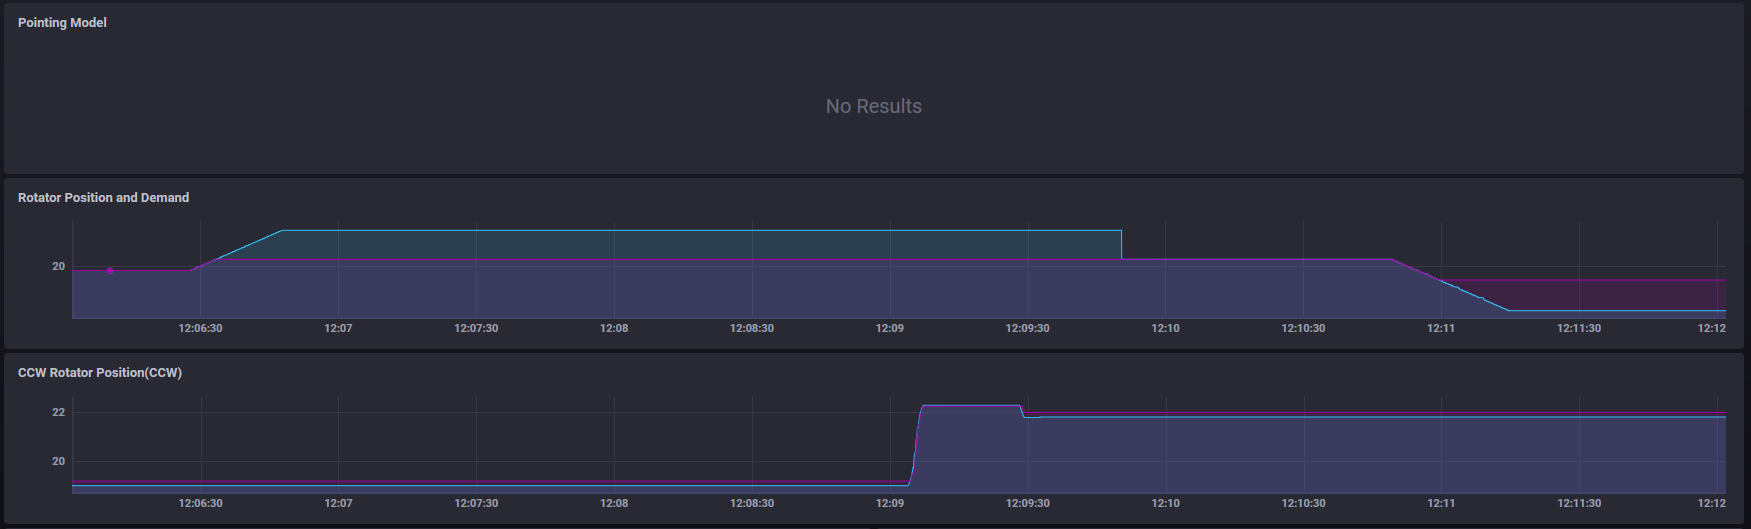
\includegraphics[width=5.20833in]{jira_imgs/1084.png}\\
\url{https://chronograf-summit-efd.lsst.codes/sources/1/dashboards/6?tempVars\%5Btest_start\%5D=START\%20-\%20Interlock\%20Rotator_CCW\%20Integration\%20Test\&tempVars\%5Btest_end\%5D=END\%20-\%20Interlock\%20Rotator_CCW\%20Integration\%20Test\&lower=now\%28\%29\%20-\%2015m}

\medskip }
\end{minipage} \\ \cdashline{2-2}

 & Status: \textbf{ Initial Pass } \\ \hline

34 & Description \\
 & \begin{minipage}[t]{15cm}
{\footnotesize
\smallskip
{With the Camera Rotator in the enabled/stationary state and both the
Camera Rotator and CCW not moving, send a \emph{positionSet} command of
0 degrees.}

\medskip }
\end{minipage}
\\ \cdashline{2-2}


 & Expected Result \\
 & \begin{minipage}[t]{15cm}{\footnotesize
\smallskip
{The Camera Rotator and the CCW do not move.}

\medskip }
\end{minipage} \\ \cdashline{2-2}

 & Actual Result \\
 & \begin{minipage}[t]{15cm}{\footnotesize
\smallskip
Deviation: We used a fixed position track command because the CCW was
not subscribed to the \emph{positionSet} or the \emph{move} commands.

\medskip }
\end{minipage} \\ \cdashline{2-2}

 & Issues found executing this step:  \\
 & \begin{minipage}[t]{13cm}{\footnotesize
\smallskip
\href{https://jira.lsstcorp.org/browse/LVV-18473}{LVV-18473}~~The CCW and Camera Rotator are only able to be moved synchronously with
a track command

\medskip }
\end{minipage} \\ \cdashline{2-2}
 & Status: \textbf{ Fail } \\ \hline

35 & Description \\
 & \begin{minipage}[t]{15cm}
{\footnotesize
\smallskip
{Send a \emph{move} command}

\medskip }
\end{minipage}
\\ \cdashline{2-2}


 & Expected Result \\
 & \begin{minipage}[t]{15cm}{\footnotesize
\smallskip
{The Camera Rotator and the CCW are at 0 degrees.}

\medskip }
\end{minipage} \\ \cdashline{2-2}

 & Actual Result \\
 & \begin{minipage}[t]{15cm}{\footnotesize
\smallskip
Deviation: As stated in the step before, we used the \emph{startTrack}
and \emph{track} commands to move back to 0 degrees.

\medskip }
\end{minipage} \\ \cdashline{2-2}

 & Issues found executing this step:  \\
 & \begin{minipage}[t]{13cm}{\footnotesize
\smallskip
\href{https://jira.lsstcorp.org/browse/LVV-18473}{LVV-18473}~~The CCW and Camera Rotator are only able to be moved synchronously with
a track command

\medskip }
\end{minipage} \\ \cdashline{2-2}
 & Status: \textbf{ Fail } \\ \hline

36 & Description \\
 & \begin{minipage}[t]{15cm}
{\footnotesize
\smallskip
{Send a \emph{velocitySet} command of +0.02\textbf{~}deg/s.}

\medskip }
\end{minipage}
\\ \cdashline{2-2}


 & Expected Result \\
 & \begin{minipage}[t]{15cm}{\footnotesize
\smallskip
{The Camera Rotator and CCW do not move.}

\medskip }
\end{minipage} \\ \cdashline{2-2}

 & Actual Result \\
 & \begin{minipage}[t]{15cm}{\footnotesize
\smallskip
{The velocity parameter that was used was actually +0.5deg/s.}

\medskip }
\end{minipage} \\ \cdashline{2-2}

 & Status: \textbf{ Initial Pass } \\ \hline

37 & Description \\
 & \begin{minipage}[t]{15cm}
{\footnotesize
\smallskip
{Send a \emph{move} command}

\medskip }
\end{minipage}
\\ \cdashline{2-2}


 & Expected Result \\
 & \begin{minipage}[t]{15cm}{\footnotesize
\smallskip
{The Camera Rotator begins to move while the CCW remains idle.}

\medskip }
\end{minipage} \\ \cdashline{2-2}

 & Actual Result \\
 & \begin{minipage}[t]{15cm}{\footnotesize
\smallskip
{Initially, the plan was to send a \emph{moveConstantVelocity} command
for 0.02deg/s for a \emph{moveDuration~}of 115 seconds to test if the
positive limit switch of the synchronous motion assembly would be
tripped within the +2.2 degrees. However, we used the
\emph{move~}command because the moveConstantVelocity was not implemented
in the LSST CSC and the positive limit switch was not tripped at +2.2
degrees. As a result, we used the \emph{positionSet} command to move +10
degrees to determine the actual distance necessary to trip the positive
limit switch.}

\medskip }
\end{minipage} \\ \cdashline{2-2}

 & Status: \textbf{ Initial Pass } \\ \hline

38 & Description \\
 & \begin{minipage}[t]{15cm}
{\footnotesize
\smallskip
{Verify the positive limit switch is tripped on the synchronous motion
assembly.}\\
{\\
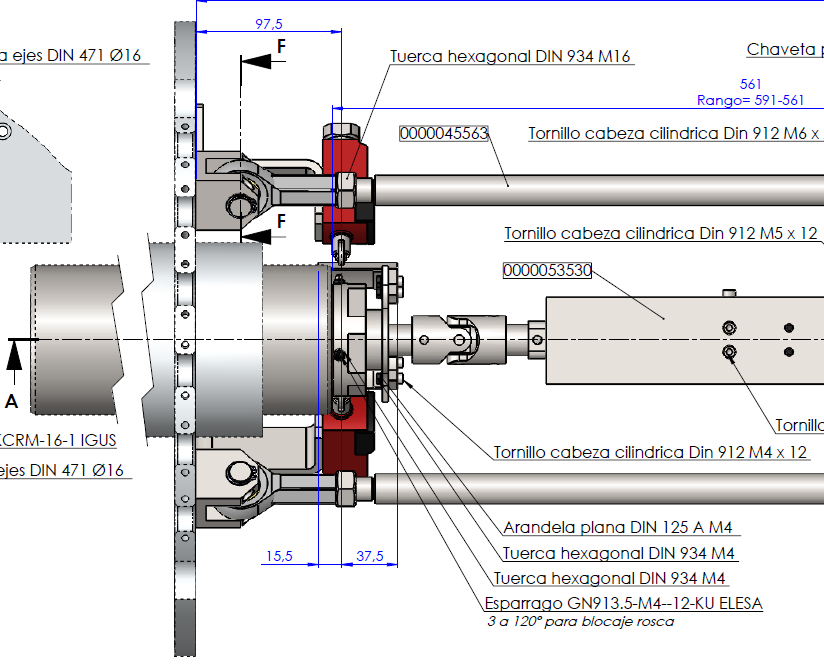
\includegraphics[width=3.12500in]{jira_imgs/1032.png}~}

\medskip }
\end{minipage}
\\ \cdashline{2-2}


 & Expected Result \\
 & \begin{minipage}[t]{15cm}{\footnotesize
\smallskip
{The fault triggered on the synchronous motion positive limit switch
disables the drives on both the Camera Rotator and CCW drives by a Safe
Torque Off trigger.}

\medskip }
\end{minipage} \\ \cdashline{2-2}

 & Actual Result \\
 & \begin{minipage}[t]{15cm}{\footnotesize
\smallskip
The positive limit switch was successfully tripped and as a result,
disabled the drives on the CCW and Camera Rotator.

\medskip }
\end{minipage} \\ \cdashline{2-2}

 & Status: \textbf{ Initial Pass } \\ \hline

39 & Description \\
 & \begin{minipage}[t]{15cm}
{\footnotesize
\smallskip
Verify the location of the positive limit switch is equal to or less
than 2.2 degrees.

\medskip }
\end{minipage}
\\ \cdashline{2-2}


 & Expected Result \\
 & \begin{minipage}[t]{15cm}{\footnotesize
\smallskip
The Camera Rotator is within 2.2 degrees of the CCW.~

\medskip }
\end{minipage} \\ \cdashline{2-2}

 & Actual Result \\
 & \begin{minipage}[t]{15cm}{\footnotesize
\smallskip
{This was tested at least 3 times and as a result, it was consistently
seen that the positive limit switch was being tripped at approximately
2.7 degrees.}

\medskip }
\end{minipage} \\ \cdashline{2-2}

 & Issues found executing this step:  \\
 & \begin{minipage}[t]{13cm}{\footnotesize
\smallskip
\href{https://jira.lsstcorp.org/browse/LVV-18475}{LVV-18475}~~Synchronous motion positive limit switch over +2.2 degrees

\medskip }
\end{minipage} \\ \cdashline{2-2}
 & Status: \textbf{ Fail } \\ \hline

40 & Description \\
 & \begin{minipage}[t]{15cm}
{\footnotesize
\smallskip
Reset the synchronous motion interlock.

\medskip }
\end{minipage}
\\ \cdashline{2-2}


 & Expected Result \\
 & \begin{minipage}[t]{15cm}{\footnotesize
\smallskip
{The Camera Rotator and CCW drives are both on and are in the Enabled
State.}

\medskip }
\end{minipage} \\ \cdashline{2-2}

 & Actual Result \\
 & \begin{minipage}[t]{15cm}{\footnotesize
\smallskip
To reset the synchronous motion interlock, we had to move the CCW to
-0.5 degrees in order to get the CAM off the positive limit switch,
clear the interlock switch from the CCW, clear the Camera Rotator and
then move both back to 0 degrees.

\medskip }
\end{minipage} \\ \cdashline{2-2}

 & Issues found executing this step:  \\
 & \begin{minipage}[t]{13cm}{\footnotesize
\smallskip
\href{https://jira.lsstcorp.org/browse/LVV-18476}{LVV-18476}~~Synchronous Motion Interlock Reset

\medskip }
\end{minipage} \\ \cdashline{2-2}
 & Status: \textbf{ Fail } \\ \hline

41 & Description \\
 & \begin{minipage}[t]{15cm}
{\footnotesize
\smallskip
{With the Camera Rotator in the enabled/stationary state and both the
Camera Rotator and CCW not moving, send a \emph{positionSet} command of
0 degrees.}

\medskip }
\end{minipage}
\\ \cdashline{2-2}


 & Expected Result \\
 & \begin{minipage}[t]{15cm}{\footnotesize
\smallskip
{The Camera Rotator and the CCW do not move.}

\medskip }
\end{minipage} \\ \cdashline{2-2}

 & Actual Result \\
 & \begin{minipage}[t]{15cm}{\footnotesize
\smallskip
Deviation: As previously stated, we had to use a fixed track command
since the CCW doesn't subscribe to the \emph{positionSet} or \emph{move}
command.

\medskip }
\end{minipage} \\ \cdashline{2-2}

 & Issues found executing this step:  \\
 & \begin{minipage}[t]{13cm}{\footnotesize
\smallskip
\href{https://jira.lsstcorp.org/browse/LVV-18473}{LVV-18473}~~The CCW and Camera Rotator are only able to be moved synchronously with
a track command

\medskip }
\end{minipage} \\ \cdashline{2-2}
 & Status: \textbf{ Fail } \\ \hline

42 & Description \\
 & \begin{minipage}[t]{15cm}
{\footnotesize
\smallskip
{Send a \emph{move} command.}

\medskip }
\end{minipage}
\\ \cdashline{2-2}


 & Expected Result \\
 & \begin{minipage}[t]{15cm}{\footnotesize
\smallskip
{The Camera Rotator moves back to exactly 0 degrees and the CCW does not
move.}

\medskip }
\end{minipage} \\ \cdashline{2-2}

 & Actual Result \\
 & \begin{minipage}[t]{15cm}{\footnotesize
\smallskip
Deviation: As stated in the step before, we used the
\emph{startTrack~}and \emph{track~}commands to move back to 0 degrees.

\medskip }
\end{minipage} \\ \cdashline{2-2}

 & Issues found executing this step:  \\
 & \begin{minipage}[t]{13cm}{\footnotesize
\smallskip
\href{https://jira.lsstcorp.org/browse/LVV-18473}{LVV-18473}~~The CCW and Camera Rotator are only able to be moved synchronously with
a track command

\medskip }
\end{minipage} \\ \cdashline{2-2}
 & Status: \textbf{ Fail } \\ \hline

43 & Description \\
 & \begin{minipage}[t]{15cm}
{\footnotesize
\smallskip
{Send a \emph{velocitySet} command of -0.02\textbf{~}deg/s.\\
}{\\
}

\medskip }
\end{minipage}
\\ \cdashline{2-2}


 & Expected Result \\
 & \begin{minipage}[t]{15cm}{\footnotesize
\smallskip
{The Camera Rotator and CCW do not move.}

\medskip }
\end{minipage} \\ \cdashline{2-2}

 & Actual Result \\
 & \begin{minipage}[t]{15cm}{\footnotesize
\smallskip
The velocity used was -0.5 deg/s

\medskip }
\end{minipage} \\ \cdashline{2-2}

 & Status: \textbf{ Initial Pass } \\ \hline

44 & Description \\
 & \begin{minipage}[t]{15cm}
{\footnotesize
\smallskip
{Send a \emph{move} command}

\medskip }
\end{minipage}
\\ \cdashline{2-2}


 & Expected Result \\
 & \begin{minipage}[t]{15cm}{\footnotesize
\smallskip
{The Camera Rotator begins to move while the CCW remains idle.}

\medskip }
\end{minipage} \\ \cdashline{2-2}

 & Actual Result \\
 & \begin{minipage}[t]{15cm}{\footnotesize
\smallskip
After seeing the positive limit switch was not tripped at +2.2 degrees,
the negative limit switch was tested by sending
a\emph{~positionSet~}command of -10 degrees.

\medskip }
\end{minipage} \\ \cdashline{2-2}

 & Issues found executing this step:  \\
 & \begin{minipage}[t]{13cm}{\footnotesize
\smallskip
\href{https://jira.lsstcorp.org/browse/LVV-18477}{LVV-18477}~~Synchronous Motion Negative Limit Switch over -2.2 degrees

\medskip }
\end{minipage} \\ \cdashline{2-2}
 & Status: \textbf{ Fail } \\ \hline

45 & Description \\
 & \begin{minipage}[t]{15cm}
{\footnotesize
\smallskip
{Verify the negative limit switch is tripped on the synchronous motion
assembly.}\\
{\\
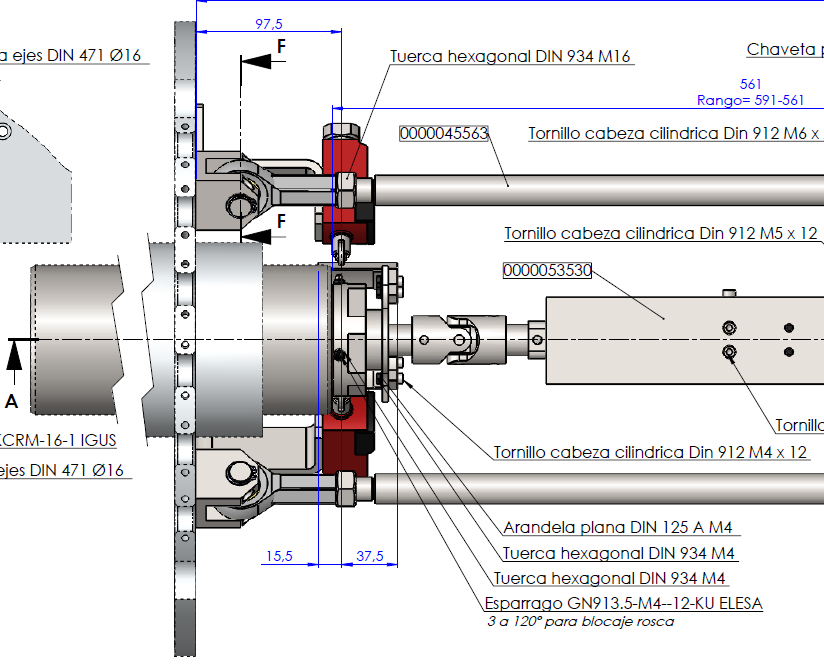
\includegraphics[width=3.12500in]{jira_imgs/1032.png}~}

\medskip }
\end{minipage}
\\ \cdashline{2-2}


 & Expected Result \\
 & \begin{minipage}[t]{15cm}{\footnotesize
\smallskip
{The fault triggered on the synchronous motion negative limit switch
disables the drives on both the Camera Rotator and CCW drives by a Safe
Torque Off trigger.}

\medskip }
\end{minipage} \\ \cdashline{2-2}

 & Actual Result \\
 & \begin{minipage}[t]{15cm}{\footnotesize
\smallskip
The negative limit switch synchronous motion assembly was tripped and
correctly disabled the drives on both the Camera Rotator and CCW.

\medskip }
\end{minipage} \\ \cdashline{2-2}

 & Status: \textbf{ Initial Pass } \\ \hline

46 & Description \\
 & \begin{minipage}[t]{15cm}
{\footnotesize
\smallskip
Verify the location of the negative limit switch is equal to or less
than 2.2 degrees.

\medskip }
\end{minipage}
\\ \cdashline{2-2}


 & Expected Result \\
 & \begin{minipage}[t]{15cm}{\footnotesize
\smallskip
The Camera Rotator is within 2.2 degrees of the CCW.

\medskip }
\end{minipage} \\ \cdashline{2-2}

 & Actual Result \\
 & \begin{minipage}[t]{15cm}{\footnotesize
\smallskip
This was tested multiple times and the negative limit switch was seen to
be consistently tripped at -5.19 degrees.

\medskip }
\end{minipage} \\ \cdashline{2-2}

 & Issues found executing this step:  \\
 & \begin{minipage}[t]{13cm}{\footnotesize
\smallskip
\href{https://jira.lsstcorp.org/browse/LVV-18477}{LVV-18477}~~Synchronous Motion Negative Limit Switch over -2.2 degrees

\medskip }
\end{minipage} \\ \cdashline{2-2}
 & Status: \textbf{ Fail } \\ \hline

47 & Description \\
 & \begin{minipage}[t]{15cm}
{\footnotesize
\smallskip
Reset the synchronous motion interlock.

\medskip }
\end{minipage}
\\ \cdashline{2-2}


 & Expected Result \\
 & \begin{minipage}[t]{15cm}{\footnotesize
\smallskip
{The Camera Rotator and CCW drives are both on and are in the Enabled
State.}

\medskip }
\end{minipage} \\ \cdashline{2-2}

 & Actual Result \\
 & \begin{minipage}[t]{15cm}{\footnotesize
\smallskip
To reset the synchronous motion interlock, we had to move the CCW to
-0.5 degrees in order to get the CAM off the positive limit switch,
clear the interlock switch from the CCW, clear the Camera Rotator and
then move both back to 0 degrees.

\medskip }
\end{minipage} \\ \cdashline{2-2}

 & Issues found executing this step:  \\
 & \begin{minipage}[t]{13cm}{\footnotesize
\smallskip
\href{https://jira.lsstcorp.org/browse/LVV-18476}{LVV-18476}~~Synchronous Motion Interlock Reset

\medskip }
\end{minipage} \\ \cdashline{2-2}
 & Status: \textbf{ Fail } \\ \hline

48 & Description \\
 & \begin{minipage}[t]{15cm}
{\footnotesize
\smallskip
{With the Camera Rotator in the enabled/stationary state and both the
Camera Rotator and CCW not moving, send a \emph{positionSet} command of
0 degrees.}

\medskip }
\end{minipage}
\\ \cdashline{2-2}


 & Expected Result \\
 & \begin{minipage}[t]{15cm}{\footnotesize
\smallskip
{The Camera Rotator and the CCW do not move.}

\medskip }
\end{minipage} \\ \cdashline{2-2}

 & Actual Result \\
 & \begin{minipage}[t]{15cm}{\footnotesize
\smallskip
In preparation for the next test, the Camera Rotator was given a track
command to a fixed position of 0 degrees.

\medskip }
\end{minipage} \\ \cdashline{2-2}

 & Issues found executing this step:  \\
 & \begin{minipage}[t]{13cm}{\footnotesize
\smallskip
\href{https://jira.lsstcorp.org/browse/LVV-18473}{LVV-18473}~~The CCW and Camera Rotator are only able to be moved synchronously with
a track command

\medskip }
\end{minipage} \\ \cdashline{2-2}
 & Status: \textbf{ Fail } \\ \hline

49 & Description \\
 & \begin{minipage}[t]{15cm}
{\footnotesize
\smallskip
{Send a \emph{move} command}

\medskip }
\end{minipage}
\\ \cdashline{2-2}


 & Expected Result \\
 & \begin{minipage}[t]{15cm}{\footnotesize
\smallskip
{The Camera Rotator moves to 0 degrees while the CCW remains idle.}

\medskip }
\end{minipage} \\ \cdashline{2-2}

 & Actual Result \\
 & \begin{minipage}[t]{15cm}{\footnotesize
\smallskip
The Camera Rotator and CCW were both positioned to 0 degrees using the
\emph{track} command.

\medskip }
\end{minipage} \\ \cdashline{2-2}

 & Issues found executing this step:  \\
 & \begin{minipage}[t]{13cm}{\footnotesize
\smallskip
\href{https://jira.lsstcorp.org/browse/LVV-18473}{LVV-18473}~~The CCW and Camera Rotator are only able to be moved synchronously with
a track command

\medskip }
\end{minipage} \\ \cdashline{2-2}
 & Status: \textbf{ Fail } \\ \hline

50 & Description \\
 & \begin{minipage}[t]{15cm}
{\footnotesize
\smallskip
\textbf{{Hard Breaking E-Stop Test}}\\
{The following steps define what the Jupyter Notebook for this test case
implements. Executing the Jupyter notebook is the only actual step that
needs to be executed.}\textbf{{~}}

\medskip }
\end{minipage}
\\ \cdashline{2-2}


 & Expected Result \\
 & \begin{minipage}[t]{15cm}{\footnotesize
\smallskip
The Jupyter notebook controls the system to run through the steps below.

\medskip }
\end{minipage} \\ \cdashline{2-2}

 & Actual Result \\
 & \begin{minipage}[t]{15cm}{\footnotesize
\smallskip
We successfully ran the Jupyter notebook which allowed proper control of
the system.\\[2\baselineskip]For the EFD plot of the final run of the
E-STop Test, see the attached picture or follow the link:\\
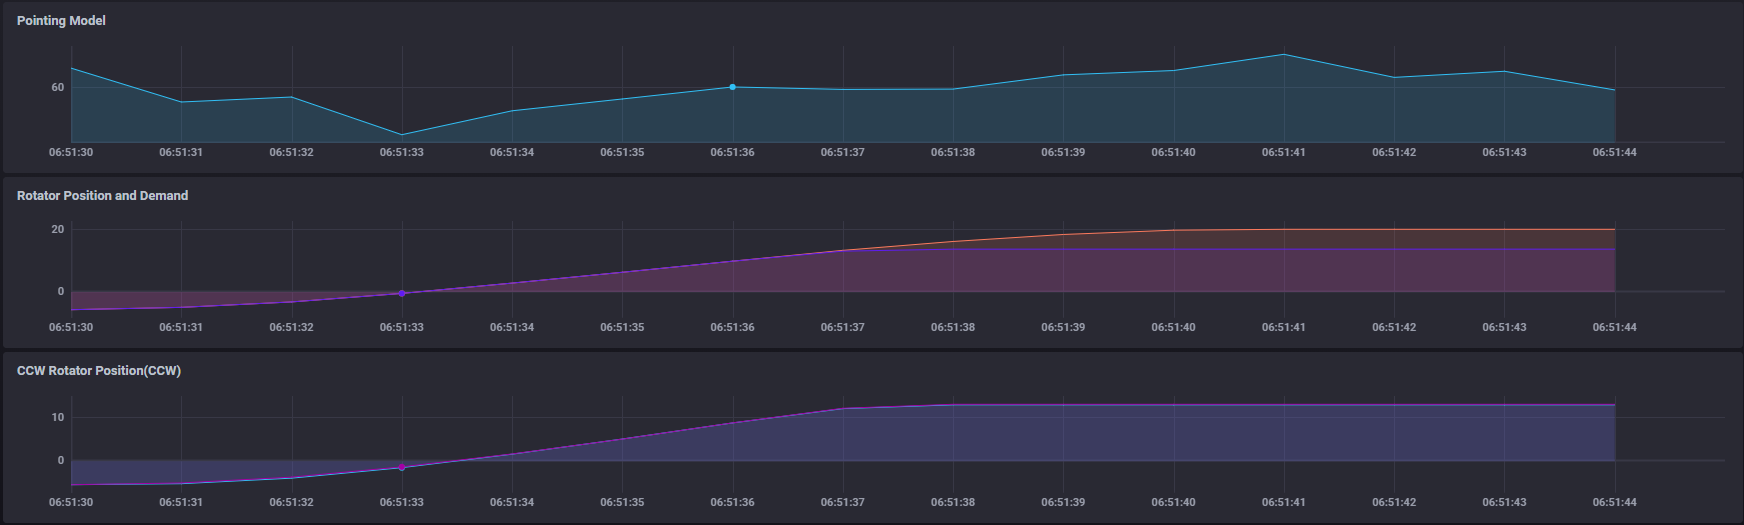
\includegraphics[width=5.20833in]{jira_imgs/1085.png}\\
\url{https://chronograf-summit-efd.lsst.codes/sources/1/dashboards/6?tempVars\%5Btest_start\%5D=START\%20-\%20E-Stop\%20MTPtg_Rotator_CCW\%20Integration\%20Test\&tempVars\%5Btest_end\%5D=END\%20-\%20E-Stop\%20MTPtg_Rotator_CCW\%20Integration\%20Test\&lower=now\%28\%29\%20-\%2015m\#}

\medskip }
\end{minipage} \\ \cdashline{2-2}

 & Status: \textbf{ Initial Pass } \\ \hline

51 & Description \\
 & \begin{minipage}[t]{15cm}
{\footnotesize
\smallskip
Send \emph{trackStart} Command~

\medskip }
\end{minipage}
\\ \cdashline{2-2}


 & Expected Result \\
 & \begin{minipage}[t]{15cm}{\footnotesize
\smallskip
The Camera Rotator transitions from the Enabled/Stationary state to the
Enabled/SlewingAndTracking state.

\medskip }
\end{minipage} \\ \cdashline{2-2}

 & Actual Result \\
 & \begin{minipage}[t]{15cm}{\footnotesize
\smallskip
We sent a trackStart to a fixed position through the Ptg component and
saw that the Camera Rotator successfully transitioned into the
SlewingAndTracking state.

\medskip }
\end{minipage} \\ \cdashline{2-2}

 & Status: \textbf{ Initial Pass } \\ \hline

52 & Description \\
 & \begin{minipage}[t]{15cm}
{\footnotesize
\smallskip
Send a \emph{track} command

\medskip }
\end{minipage}
\\ \cdashline{2-2}


 & Expected Result \\
 & \begin{minipage}[t]{15cm}{\footnotesize
\smallskip
The Camera Rotator starts it's rotation and the CCW synchronizes with
this rotation.

\medskip }
\end{minipage} \\ \cdashline{2-2}

 & Actual Result \\
 & \begin{minipage}[t]{15cm}{\footnotesize
\smallskip
The Camera Rotator and CCW both begin to follow the track command.

\medskip }
\end{minipage} \\ \cdashline{2-2}

 & Status: \textbf{ Initial Pass } \\ \hline

53 & Description \\
 & \begin{minipage}[t]{15cm}
{\footnotesize
\smallskip
Hit the E-Stop

\medskip }
\end{minipage}
\\ \cdashline{2-2}


 & Expected Result \\
 & \begin{minipage}[t]{15cm}{\footnotesize
\smallskip
The Camera Rotator and CCW both stop their rotation.

\medskip }
\end{minipage} \\ \cdashline{2-2}

 & Actual Result \\
 & \begin{minipage}[t]{15cm}{\footnotesize
\smallskip
Once the CCW and Camera Rotator were seen to be moving at their maximum
velocity, the E-stop was pressed.

\medskip }
\end{minipage} \\ \cdashline{2-2}

 & Status: \textbf{ Initial Pass } \\ \hline

54 & Description \\
 & \begin{minipage}[t]{15cm}
{\footnotesize
\smallskip
Using the position telemetry in the EFD, verify that the CCW and Camera
Rotator are stopped at the same position.~~

\medskip }
\end{minipage}
\\ \cdashline{2-2}


 & Expected Result \\
 & \begin{minipage}[t]{15cm}{\footnotesize
\smallskip
The CCW and Camera Rotator do not exceed the +/- 2.2 degrees difference
in position.

\medskip }
\end{minipage} \\ \cdashline{2-2}

 & Actual Result \\
 & \begin{minipage}[t]{15cm}{\footnotesize
\smallskip
The CCW was stopped at 13.1 degrees while the Camera Rotator was stopped
at 13.84 degrees.~

\medskip }
\end{minipage} \\ \cdashline{2-2}

 & Status: \textbf{ Initial Pass } \\ \hline

55 & Description \\
 & \begin{minipage}[t]{15cm}
{\footnotesize
\smallskip
Shutdown the CCW and Camera Rotator.

\medskip }
\end{minipage}
\\ \cdashline{2-2}


 & Expected Result \\
 & \begin{minipage}[t]{15cm}{\footnotesize
\smallskip
The CCW and Camera Rotator are shutdown.

\medskip }
\end{minipage} \\ \cdashline{2-2}

 & Actual Result \\
 & \begin{minipage}[t]{15cm}{\footnotesize
\smallskip
The CCW and Camera Rotator were not shut down at the end of testing
because of how long it takes to restart the system; Therefore, the
E-stop is pressed and the systems are left in FAULT at the end of every
day.

\medskip }
\end{minipage} \\ \cdashline{2-2}

 & Status: \textbf{ Initial Pass } \\ \hline

\end{longtable}

\paragraph{Test Case LVV-T1588 - Pointing Component Control Test
 }\mbox{}\\

Open  \href{https://jira.lsstcorp.org/secure/Tests.jspa#/testCase/LVV-T1588}{\textit{ LVV-T1588 } }
test case in Jira.

The objective of this test case is to verify the combined control of the
integrated CCW and Camera Rotator via the LSST pointing component as
specified in \citeds{LTS-218}. This test case will exercise the functionality of
the synchronized CCW and Camera Rotator during tracking and move
commands and meeting the following criteria:

\begin{itemize}
\tightlist
\item
  Does \textbf{NOT} require the Camera Rotator to be loaded with the
  camera simulated mass or actual camera hardware
\end{itemize}

This test case will execute 4 scenarios:

\begin{enumerate}
\tightlist
\item
  Basic Control Scenario
\item
  High Rotation Stress Test Scenario

  \begin{itemize}
  \tightlist
  \item
    Full operational range of motion from +90 to -90
  \end{itemize}
\item
  Filter Change Scenario
\item
  Typical Night

  \begin{itemize}
  \tightlist
  \item
    Verify the CCW does not rotate during exposure
  \item
    Execute an extended exposure
  \end{itemize}
\end{enumerate}


\textbf{ Preconditions}:\\
Prior to the execution of this test case to verify the pointing
component of the CCW + Camera Rotator, the following Summit tasks must
be completed:

\begin{itemize}
\tightlist
\item
  The CCW has been installed on the Camera Cart

  \begin{itemize}
  \tightlist
  \item
    \url{https://jira.lsstcorp.org/browse/SUMMIT-2156}
  \end{itemize}
\item
  The Camera Hexapod/Rotator Controller has been deployed on the summit

  \begin{itemize}
  \tightlist
  \item
    \url{https://jira.lsstcorp.org/browse/SUMMIT-3229}
  \end{itemize}
\item
  The Combined Motion of the CCW + Rotator has been verified to be in
  sync

  \begin{itemize}
  \tightlist
  \item
    \url{https://jira.lsstcorp.org/browse/SUMMIT-3295}
  \end{itemize}
\item
  A provisional linkage is installed between the Camera Rotator and the
  CCW

  \begin{itemize}
  \tightlist
  \item
    \url{https://jira.lsstcorp.org/browse/SUMMIT-3481}
  \end{itemize}
\end{itemize}


Execution status: {\bf Fail }

Final comment:\\


Detailed steps results:

\begin{longtable}{p{1cm}p{15cm}}
\hline
{Step} & Step Details\\ \hline
1 & Description \\
 & \begin{minipage}[t]{15cm}
{\footnotesize
\smallskip
\textbf{STARTING THE EUI}\\[2\baselineskip]Double click the Hexapod GUI
Viewer desktop icon on the computer.

\begin{itemize}
\tightlist
\item
  This can be done on the Dell Management PC or another computer on the
  same network
\end{itemize}

\medskip }
\end{minipage}
\\ \cdashline{2-2}


 & Expected Result \\
 & \begin{minipage}[t]{15cm}{\footnotesize
\smallskip
A prompt to enter a password is shown.~

\medskip }
\end{minipage} \\ \cdashline{2-2}

 & Actual Result \\
 & \begin{minipage}[t]{15cm}{\footnotesize
\smallskip
This was previously verified in the\emph{~Integration of Camera Rotator
with SAL 4.0 (LSST)~}Test Case.

\medskip }
\end{minipage} \\ \cdashline{2-2}

 & Status: \textbf{ Initial Pass } \\ \hline

2 & Description \\
 & \begin{minipage}[t]{15cm}
{\footnotesize
\smallskip
Enter the password ``lsst-vnc''

\begin{itemize}
\tightlist
\item
  If the EUI isn't automatically up and running when the VNC opens,
  double click on the CAM\_Hex\_eGUI or M2\_Hex\_eGUI icon on the VNC
  viewer
\end{itemize}

\medskip }
\end{minipage}
\\ \cdashline{2-2}


 & Expected Result \\
 & \begin{minipage}[t]{15cm}{\footnotesize
\smallskip
The EUI is in the Offline State/PublishOnly substate and is able to
publish through SAL but cannot receive commands.

\medskip }
\end{minipage} \\ \cdashline{2-2}

 & Actual Result \\
 & \begin{minipage}[t]{15cm}{\footnotesize
\smallskip
This was previously verified in the\emph{~Integration of Camera Rotator
with SAL 4.0 (LSST)~}Test Case.

\medskip }
\end{minipage} \\ \cdashline{2-2}

 & Status: \textbf{ Initial Pass } \\ \hline

3 & Description \\
 & \begin{minipage}[t]{15cm}
{\footnotesize
\smallskip
\textbf{OFFLINESTATE/AVAILABLESTATE}\\
On the Main tab, select the ``Offline SubState Cmd'' field in the
Commands to Send section, set the Offline SubState Triggers to ``System
Ready'' and click on the Send Command button.\\
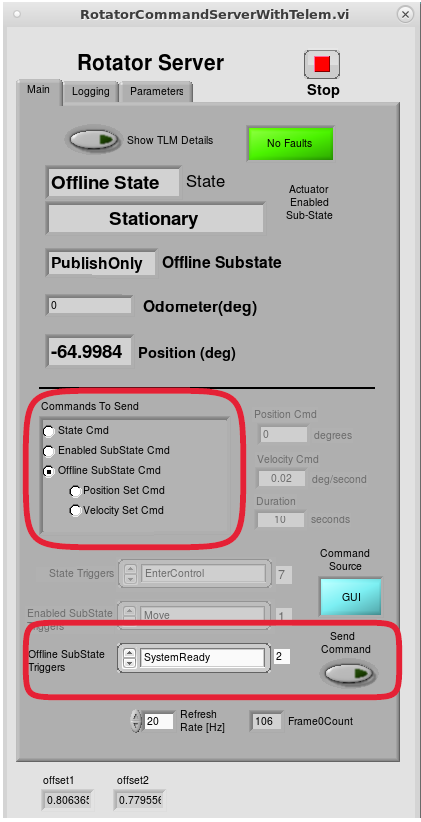
\includegraphics[width=1.79167in]{jira_imgs/1005.png}

\medskip }
\end{minipage}
\\ \cdashline{2-2}


 & Expected Result \\
 & \begin{minipage}[t]{15cm}{\footnotesize
\smallskip
The system transitions from the OfflineState/PublishOnly substate to the
OfflineState/AvailableState
substate.\\[2\baselineskip]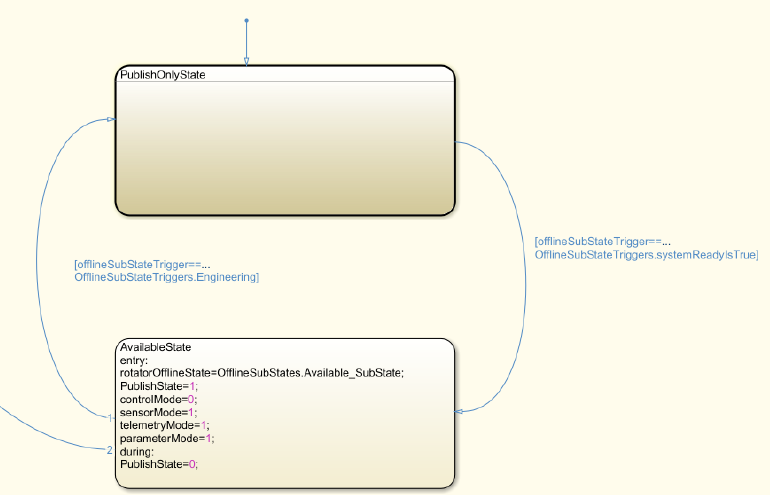
\includegraphics[width=1.79167in]{jira_imgs/1007.png}

\medskip }
\end{minipage} \\ \cdashline{2-2}

 & Actual Result \\
 & \begin{minipage}[t]{15cm}{\footnotesize
\smallskip
This was previously verified in the\emph{~Integration of Camera Rotator
with SAL 4.0 (LSST)~}Test Case.

\medskip }
\end{minipage} \\ \cdashline{2-2}

 & Status: \textbf{ Initial Pass } \\ \hline

4 & Description \\
 & \begin{minipage}[t]{15cm}
{\footnotesize
\smallskip
\textbf{SWITCHING TO DDS MODE}\\
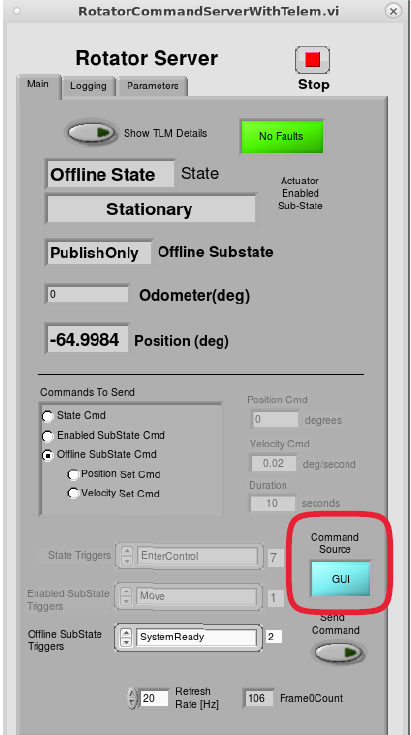
\includegraphics[width=1.79167in]{jira_imgs/1014.png}\\
If the Command Source does not show DDS, go to the Parameters tab,
select DDS under the Command Source and click the Set Command Source
button.\\
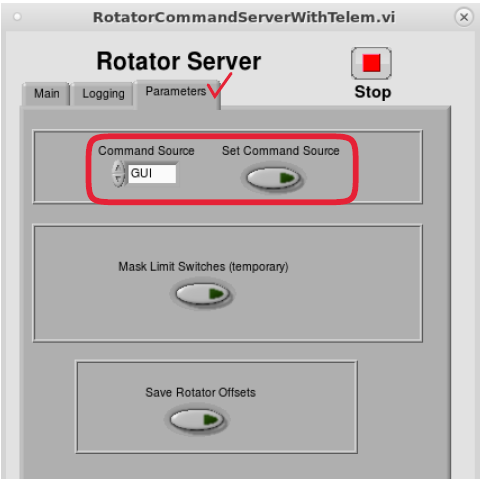
\includegraphics[width=1.79167in]{jira_imgs/1013.png}\textbf{Note:~If
the GUI is used after being set to DDS mode, the system will switch back
the Command Source to GUI and ignore any DDS commands. The Command
Source must show DDS in order to receive DDS commands.}

\medskip }
\end{minipage}
\\ \cdashline{2-2}


 & Expected Result \\
 & \begin{minipage}[t]{15cm}{\footnotesize
\smallskip
The system is capable of receiving/responding to DDS commands.

\medskip }
\end{minipage} \\ \cdashline{2-2}

 & Actual Result \\
 & \begin{minipage}[t]{15cm}{\footnotesize
\smallskip
This was previously verified in the\emph{~Integration of Camera Rotator
with SAL 4.0 (LSST)~}Test Case.

\medskip }
\end{minipage} \\ \cdashline{2-2}

 & Status: \textbf{ Initial Pass } \\ \hline

5 & Description \\
 & \begin{minipage}[t]{15cm}
{\footnotesize
\smallskip
\textbf{OFFLINESTATE -\textgreater{} STANDBYSTATE}\\
The system receives an \emph{enterControl State Transition} command
through DDS.

\medskip }
\end{minipage}
\\ \cdashline{2-2}


 & Expected Result \\
 & \begin{minipage}[t]{15cm}{\footnotesize
\smallskip
The system transitions into the StandbyState and is capable of
receiving/responding to DDS commands.\\
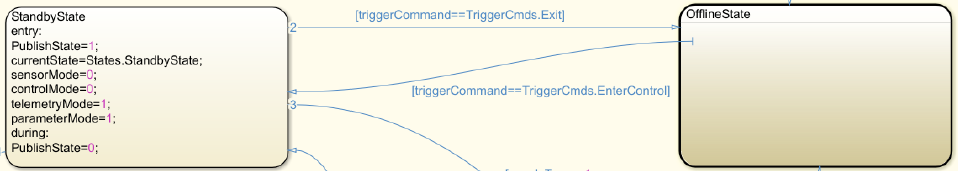
\includegraphics[width=4.68750in]{jira_imgs/1018.png}

\medskip }
\end{minipage} \\ \cdashline{2-2}

 & Actual Result \\
 & \begin{minipage}[t]{15cm}{\footnotesize
\smallskip
This was previously verified in the\emph{~Integration of Camera Rotator
with SAL 4.0 (LSST)~}Test Case.

\medskip }
\end{minipage} \\ \cdashline{2-2}

 & Status: \textbf{ Initial Pass } \\ \hline

6 & Description \\
 & \begin{minipage}[t]{15cm}
{\footnotesize
\smallskip
\textbf{STANDBYSTATE -\textgreater{} DISABLEDSTATE}\\
From the StandbyState, send a \emph{start} command through the DDS.

\medskip }
\end{minipage}
\\ \cdashline{2-2}


 & Expected Result \\
 & \begin{minipage}[t]{15cm}{\footnotesize
\smallskip
The system transitions into DisabledState after receiving/responding to
DDS command and the wrapper in the PXI real time controller looks for
the configuration file.\\
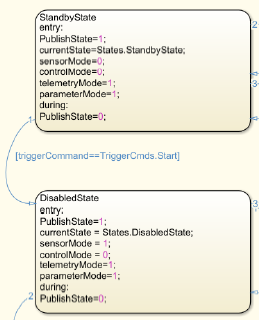
\includegraphics[width=1.79167in]{jira_imgs/1019.png}\\
If the configuration file is invalid or out of range, the system will
transition into a Fault State

\medskip }
\end{minipage} \\ \cdashline{2-2}

 & Actual Result \\
 & \begin{minipage}[t]{15cm}{\footnotesize
\smallskip
This was previously verified in the\emph{~Integration of Camera Rotator
with SAL 4.0 (LSST)~}Test Case.

\medskip }
\end{minipage} \\ \cdashline{2-2}

 & Status: \textbf{ Initial Pass } \\ \hline

7 & Description \\
 & \begin{minipage}[t]{15cm}
{\footnotesize
\smallskip
\textbf{DISABLEDSTATE -\textgreater{} ENABLEDSTATE}\\
From the DisabledState, send an \emph{enable state} command through the
DDS.

\medskip }
\end{minipage}
\\ \cdashline{2-2}


 & Expected Result \\
 & \begin{minipage}[t]{15cm}{\footnotesize
\smallskip
The system transitions into the EnabledState/Stationary substate, the
motor drives are enabled, motor brakes are released and the system is
capable of receiving/responding to DDS commands.\\
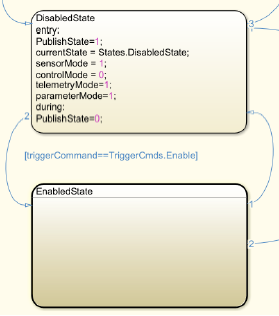
\includegraphics[width=1.79167in]{jira_imgs/1020.png}\\

\medskip }
\end{minipage} \\ \cdashline{2-2}

 & Actual Result \\
 & \begin{minipage}[t]{15cm}{\footnotesize
\smallskip
This was previously verified in the\emph{~Integration of Camera Rotator
with SAL 4.0 (LSST)~}Test Case.

\medskip }
\end{minipage} \\ \cdashline{2-2}

 & Status: \textbf{ Initial Pass } \\ \hline

8 & Description \\
 & \begin{minipage}[t]{15cm}
{\footnotesize
\smallskip
\textbf{FAULTSTATE}\\
If a Fault occurs in any of the other states, the system will
automatically transition to the Fault State. While in the Fault state,
send a \emph{clearError} command through the DDS.\\
Note: If the fault that occurs goes through the interlock system, reset
the safety relay switch and send a \emph{clearError} command.

\medskip }
\end{minipage}
\\ \cdashline{2-2}


 & Expected Result \\
 & \begin{minipage}[t]{15cm}{\footnotesize
\smallskip
The system transitions back to the OfflineState/PublishOnly substate and
is not capable of receiving/responding to DDS commands. (Go back to Step
3)\\
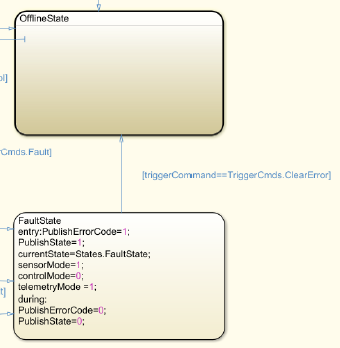
\includegraphics[width=1.79167in]{jira_imgs/1021.png}

\medskip }
\end{minipage} \\ \cdashline{2-2}

 & Actual Result \\
 & \begin{minipage}[t]{15cm}{\footnotesize
\smallskip
This was previously verified in the\emph{~Integration of Camera Rotator
with SAL 4.0 (LSST)~}Test Case.

\medskip }
\end{minipage} \\ \cdashline{2-2}

 & Status: \textbf{ Initial Pass } \\ \hline

9 & Description \\
 & \begin{minipage}[t]{15cm}
{\footnotesize
\smallskip
\textbf{{Pointing Component - Basic Control}}\\
{Insert the locking pin that so that the CCW moves synchronously to the
Camera Rotator.}

\medskip }
\end{minipage}
\\ \cdashline{2-2}


 & Expected Result \\
 & \begin{minipage}[t]{15cm}{\footnotesize
\smallskip
The CCW and Camera Rotator move synchronously to each other.

\medskip }
\end{minipage} \\ \cdashline{2-2}

 & Actual Result \\
 & \begin{minipage}[t]{15cm}{\footnotesize
\smallskip
The locking pin for the temporary linkage between the CCW and the Camera
Rotator remained inserted.

\medskip }
\end{minipage} \\ \cdashline{2-2}

 & Status: \textbf{ Initial Pass } \\ \hline

10 & Description \\
 & \begin{minipage}[t]{15cm}
{\footnotesize
\smallskip
The following steps define what the Jupyter Notebook for this test case
implements. Executing the Jupyter notebook is the only actual step that
needs to be executed.

\medskip }
\end{minipage}
\\ \cdashline{2-2}


 & Expected Result \\
 & \begin{minipage}[t]{15cm}{\footnotesize
\smallskip
The Jupyter notebook controls the system to run through the steps below.

\medskip }
\end{minipage} \\ \cdashline{2-2}

 & Actual Result \\
 & \begin{minipage}[t]{15cm}{\footnotesize
\smallskip
The Jupyter notebook was run successfully and allowed control of the
system.\\[2\baselineskip]See the attached picture from the Basic Track
Test Scenario or follow the link:\\
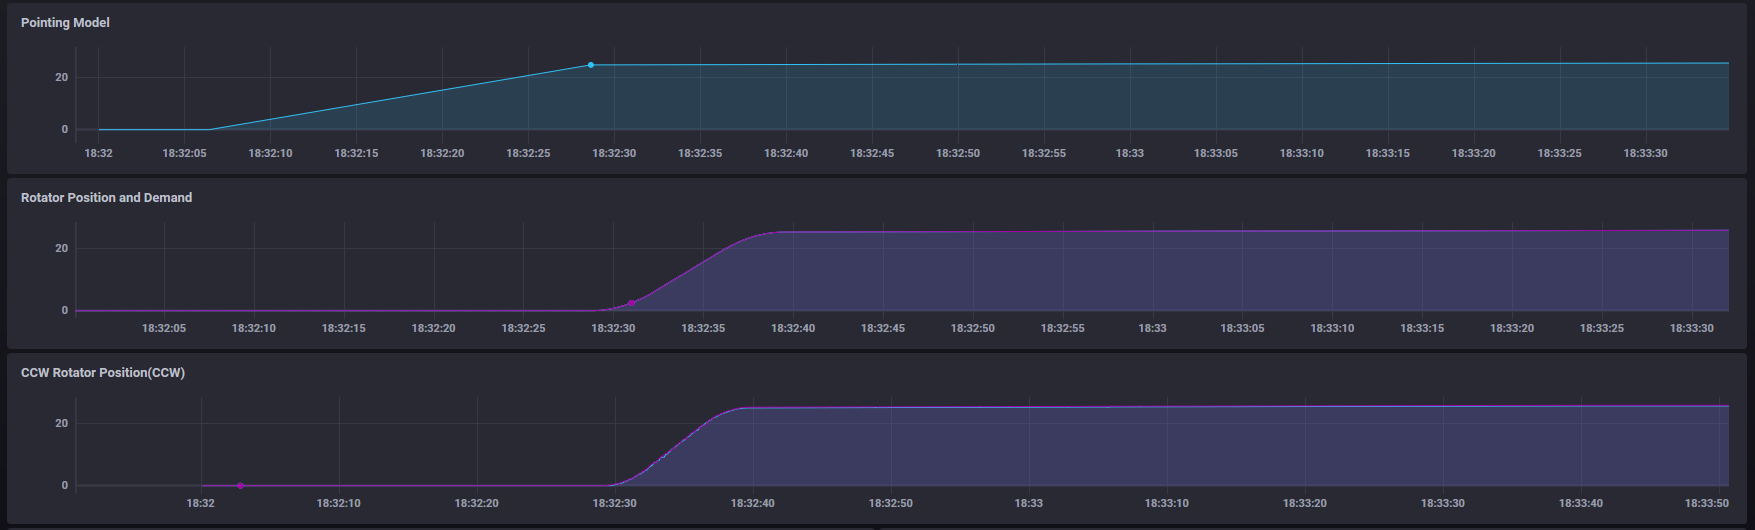
\includegraphics[width=5.20833in]{jira_imgs/1087.png}\url{https://chronograf-summit-efd.lsst.codes/sources/1/dashboards/6?tempVars\%5Btest_start\%5D=START\%20-\%20Basic\%20MTPtg\%2FRotator\%20Integration\%20Test\&tempVars\%5Btest_end\%5D=END\%20-\%20Basic\%20MTPtg\%2FRotator\%20Integration\%20Test\&lower=now\%28\%29\%20-\%2015m\#}

\medskip }
\end{minipage} \\ \cdashline{2-2}

 & Status: \textbf{ Initial Pass } \\ \hline

11 & Description \\
 & \begin{minipage}[t]{15cm}
{\footnotesize
\smallskip
Bring the Camera Rotator and the Pointing Component to the Enabled
State.

\medskip }
\end{minipage}
\\ \cdashline{2-2}


 & Expected Result \\
 & \begin{minipage}[t]{15cm}{\footnotesize
\smallskip
The Camera Rotator and Pointing Component are in the Enabled State.

\medskip }
\end{minipage} \\ \cdashline{2-2}

 & Actual Result \\
 & \begin{minipage}[t]{15cm}{\footnotesize
\smallskip
The Camera Rotator and Pointing component were successfully transitioned
into the Enabled State.

\medskip }
\end{minipage} \\ \cdashline{2-2}

 & Status: \textbf{ Initial Pass } \\ \hline

12 & Description \\
 & \begin{minipage}[t]{15cm}
{\footnotesize
\smallskip
Send a \emph{trackStart} command to the rotator.~

\medskip }
\end{minipage}
\\ \cdashline{2-2}


 & Expected Result \\
 & \begin{minipage}[t]{15cm}{\footnotesize
\smallskip
The Camera Rotator transitions from the Enabled/Stationary state to the
Enabled/SlewingAndTracking state.

\medskip }
\end{minipage} \\ \cdashline{2-2}

 & Actual Result \\
 & \begin{minipage}[t]{15cm}{\footnotesize
\smallskip
The Camera Rotator successfully transitioned into the SlewingAndTracking
state as seen on the GUI.

\medskip }
\end{minipage} \\ \cdashline{2-2}

 & Status: \textbf{ Initial Pass } \\ \hline

13 & Description \\
 & \begin{minipage}[t]{15cm}
{\footnotesize
\smallskip
Send a \emph{track} command via the pointing component to track.

\medskip }
\end{minipage}
\\ \cdashline{2-2}


 & Expected Result \\
 & \begin{minipage}[t]{15cm}{\footnotesize
\smallskip
The Camera Rotator begins to track for 30 seconds.~

\medskip }
\end{minipage} \\ \cdashline{2-2}

 & Actual Result \\
 & \begin{minipage}[t]{15cm}{\footnotesize
\smallskip
The Camera Rotator and CCW began to move synchronously.

\medskip }
\end{minipage} \\ \cdashline{2-2}

 & Status: \textbf{ Initial Pass } \\ \hline

14 & Description \\
 & \begin{minipage}[t]{15cm}
{\footnotesize
\smallskip
Send a \emph{stopTracking} command to the pointing component

\medskip }
\end{minipage}
\\ \cdashline{2-2}


 & Expected Result \\
 & \begin{minipage}[t]{15cm}{\footnotesize
\smallskip
The pointing component stops sending \emph{track} commands.

\medskip }
\end{minipage} \\ \cdashline{2-2}

 & Actual Result \\
 & \begin{minipage}[t]{15cm}{\footnotesize
\smallskip
The Pointing component stopped sending track commands.

\medskip }
\end{minipage} \\ \cdashline{2-2}

 & Status: \textbf{ Initial Pass } \\ \hline

15 & Description \\
 & \begin{minipage}[t]{15cm}
{\footnotesize
\smallskip
Send a \emph{stop} command to the Camera Rotator.

\medskip }
\end{minipage}
\\ \cdashline{2-2}


 & Expected Result \\
 & \begin{minipage}[t]{15cm}{\footnotesize
\smallskip
The Camera Rotator and CCW stop their rotation.

\medskip }
\end{minipage} \\ \cdashline{2-2}

 & Actual Result \\
 & \begin{minipage}[t]{15cm}{\footnotesize
\smallskip
A stop command was sent to the CCW first when the stopTracking command
was sent to the pointing component and then a stop command was sent to
the Camera Rotator. This order was established due to sensitivities seen
with the CCW to receive stop commands after the pointing component
stopped sending the track commands.

\medskip }
\end{minipage} \\ \cdashline{2-2}

 & Status: \textbf{ Initial Pass } \\ \hline

16 & Description \\
 & \begin{minipage}[t]{15cm}
{\footnotesize
\smallskip
{Using the position telemetry in the EFD}{, verify that the CCW and
Camera Rotator are moving synchronously.~}

\medskip }
\end{minipage}
\\ \cdashline{2-2}


 & Expected Result \\
 & \begin{minipage}[t]{15cm}{\footnotesize
\smallskip
The CCW and Camera Rotator do not exceed the +/- 2.2 degrees.

\medskip }
\end{minipage} \\ \cdashline{2-2}

 & Actual Result \\
 & \begin{minipage}[t]{15cm}{\footnotesize
\smallskip
It was seen in the position telemetry in the EFD that the CCW and CCW
were at similar positions when moving.

\medskip }
\end{minipage} \\ \cdashline{2-2}

 & Status: \textbf{ Initial Pass } \\ \hline

17 & Description \\
 & \begin{minipage}[t]{15cm}
{\footnotesize
\smallskip
\textbf{{Pointing Component- High Rotation Stress Test}}\\
The following steps define what the Jupyter Notebook for this test case
implements. Executing the Jupyter notebook is the only actual step that
needs to be executed.

\medskip }
\end{minipage}
\\ \cdashline{2-2}


 & Expected Result \\
 & \begin{minipage}[t]{15cm}{\footnotesize
\smallskip
The Jupyter notebook controls the system to run through the steps below.

\medskip }
\end{minipage} \\ \cdashline{2-2}

 & Actual Result \\
 & \begin{minipage}[t]{15cm}{\footnotesize
\smallskip
The Jupyter notebook was successfully run and correctly controls the
system.\\[2\baselineskip]See the attached picture of the High Rotation
Stress Test Scenario or follow the link:\\
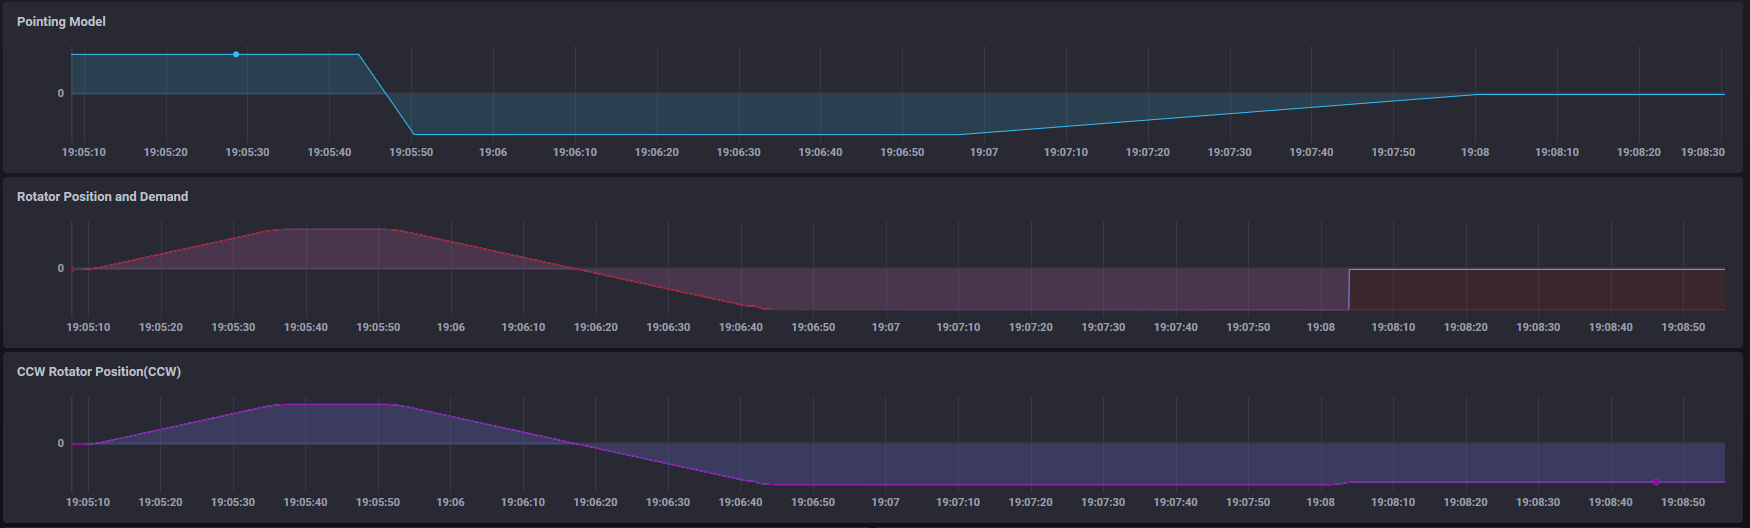
\includegraphics[width=5.20833in]{jira_imgs/1083.png}\\
\url{https://chronograf-summit-efd.lsst.codes/sources/1/dashboards/6?tempVars\%5Btest_start\%5D=START\%20-\%20High\%20Rotation\%20Stress\%20Test\&tempVars\%5Btest_end\%5D=END\%20-\%20High\%20Rotation\%20Stress\%20Test\&lower=now\%28\%29\%20-\%2015m\#}

\medskip }
\end{minipage} \\ \cdashline{2-2}

 & Status: \textbf{ Initial Pass } \\ \hline

18 & Description \\
 & \begin{minipage}[t]{15cm}
{\footnotesize
\smallskip
Bring the Camera Rotator and the Pointing Component to the Enabled
State.

\medskip }
\end{minipage}
\\ \cdashline{2-2}


 & Expected Result \\
 & \begin{minipage}[t]{15cm}{\footnotesize
\smallskip
The Camera Rotator and Pointing Component are in the Enabled State.

\medskip }
\end{minipage} \\ \cdashline{2-2}

 & Actual Result \\
 & \begin{minipage}[t]{15cm}{\footnotesize
\smallskip
The Camera Rotator was successfully transitioned into the Enabled State.

\medskip }
\end{minipage} \\ \cdashline{2-2}

 & Status: \textbf{ Initial Pass } \\ \hline

19 & Description \\
 & \begin{minipage}[t]{15cm}
{\footnotesize
\smallskip
Send a \emph{trackStart} command to the Rotator~

\medskip }
\end{minipage}
\\ \cdashline{2-2}


 & Expected Result \\
 & \begin{minipage}[t]{15cm}{\footnotesize
\smallskip
The Rotator transitions from the Enabled State/Stationary substate to
the Enabled State/Slewing and Tracking Substate.

\medskip }
\end{minipage} \\ \cdashline{2-2}

 & Actual Result \\
 & \begin{minipage}[t]{15cm}{\footnotesize
\smallskip
The Camera Rotator was correctly transitioned into the
SlewingAndTracking substate as seen on the GUI.

\medskip }
\end{minipage} \\ \cdashline{2-2}

 & Status: \textbf{ Initial Pass } \\ \hline

20 & Description \\
 & \begin{minipage}[t]{15cm}
{\footnotesize
\smallskip
Send a \emph{track} command to +90 degrees.

\medskip }
\end{minipage}
\\ \cdashline{2-2}


 & Expected Result \\
 & \begin{minipage}[t]{15cm}{\footnotesize
\smallskip
The Camera Rotator begins to track to +90 degrees.

\medskip }
\end{minipage} \\ \cdashline{2-2}

 & Actual Result \\
 & \begin{minipage}[t]{15cm}{\footnotesize
\smallskip
The Camera Rotator and CCW simultaneously moved toward +90 degrees and
started tracking.

\medskip }
\end{minipage} \\ \cdashline{2-2}

 & Status: \textbf{ Initial Pass } \\ \hline

21 & Description \\
 & \begin{minipage}[t]{15cm}
{\footnotesize
\smallskip
While the Camera Rotator is at+90 degrees, send a new \emph{track}
command to -90 degrees at 0.068deg/s.

\medskip }
\end{minipage}
\\ \cdashline{2-2}


 & Expected Result \\
 & \begin{minipage}[t]{15cm}{\footnotesize
\smallskip
The Camera Rotator and CCW synchronously move at full speed from +90
degrees to -90 degrees.

\medskip }
\end{minipage} \\ \cdashline{2-2}

 & Actual Result \\
 & \begin{minipage}[t]{15cm}{\footnotesize
\smallskip
The system reached a FAULT as the Pointing Component's demand was -90
degrees as expected, the Camera Rotator's demand was of 0 degrees
although its position never changed, and the CCW started to move in the
negative direction and tripped the interlock.

\medskip }
\end{minipage} \\ \cdashline{2-2}

 & Issues found executing this step:  \\
 & \begin{minipage}[t]{13cm}{\footnotesize
\smallskip
\href{https://jira.lsstcorp.org/browse/FRACAS-26}{FRACAS-26}~~Camera Rotator GUI Crash

\medskip }
\end{minipage} \\ \cdashline{2-2}
 & Status: \textbf{ Fail } \\ \hline

22 & Description \\
 & \begin{minipage}[t]{15cm}
{\footnotesize
\smallskip
Send a \emph{stop} command to the Camera Rotator.

\medskip }
\end{minipage}
\\ \cdashline{2-2}


 & Expected Result \\
 & \begin{minipage}[t]{15cm}{\footnotesize
\smallskip
The Camera Rotator and CCW stop their rotation.

\medskip }
\end{minipage} \\ \cdashline{2-2}

 & Actual Result \\
 & \begin{minipage}[t]{15cm}{\footnotesize
\smallskip
The Camera Rotator and CCW have already been stopped as they reached a
FAULT.

\medskip }
\end{minipage} \\ \cdashline{2-2}

 & Issues found executing this step:  \\
 & \begin{minipage}[t]{13cm}{\footnotesize
\smallskip
\href{https://jira.lsstcorp.org/browse/FRACAS-26}{FRACAS-26}~~Camera Rotator GUI Crash

\medskip }
\end{minipage} \\ \cdashline{2-2}
 & Status: \textbf{ Fail } \\ \hline

23 & Description \\
 & \begin{minipage}[t]{15cm}
{\footnotesize
\smallskip
\textbf{{Pointing Component - Filter Change}}\\
The following steps define what the Jupyter Notebook for this test case
implements. Executing the Jupyter notebook is the only actual step that
needs to be executed.

\medskip }
\end{minipage}
\\ \cdashline{2-2}


 & Expected Result \\
 & \begin{minipage}[t]{15cm}{\footnotesize
\smallskip
The Jupyter notebook controls the system to run through the steps below.

\medskip }
\end{minipage} \\ \cdashline{2-2}

 & Actual Result \\
 & \begin{minipage}[t]{15cm}{\footnotesize
\smallskip
The Jupyter notebook was successfully run and correctly controls the
system.\\[2\baselineskip]See the attached picture of the Filter Change
Test Scenario or follow the link:\\
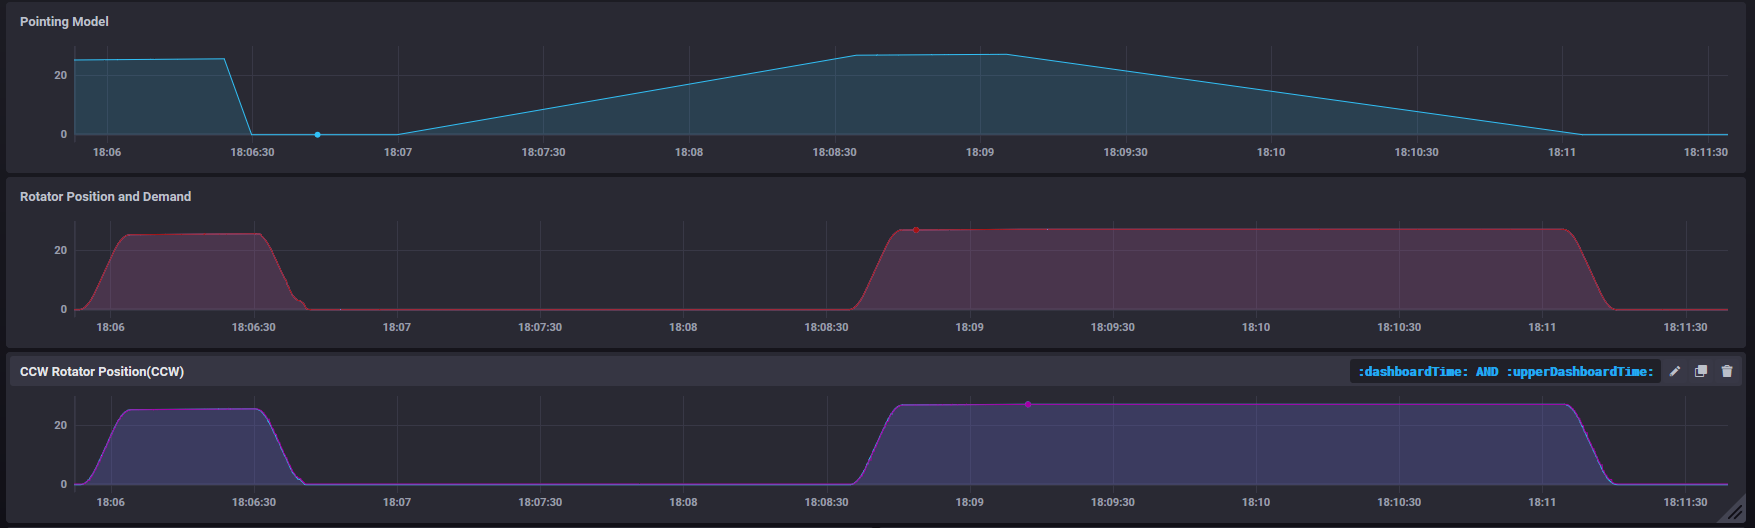
\includegraphics[width=5.20833in]{jira_imgs/1086.png}\\
\url{https://chronograf-summit-efd.lsst.codes/sources/1/dashboards/6?tempVars\%5Btest_start\%5D=START\%20-\%20Filter\%20Change\%20MTPtg_Rotator_CCW\%20Integration\%20Test\&tempVars\%5Btest_end\%5D=END\%20-\%20Filter\%20Change\%20MTPtg_Rotator_CCW\%20Integration\%20Test\&lower=now\%28\%29\%20-\%2015m\#}

\medskip }
\end{minipage} \\ \cdashline{2-2}

 & Status: \textbf{ Initial Pass } \\ \hline

24 & Description \\
 & \begin{minipage}[t]{15cm}
{\footnotesize
\smallskip
With the Camera Rotator and CCW in the Enabled state, send a
\emph{trackStart} command to the rotator.

\medskip }
\end{minipage}
\\ \cdashline{2-2}


 & Expected Result \\
 & \begin{minipage}[t]{15cm}{\footnotesize
\smallskip
The Camera Rotator transitions from the Enabled/Stationary state to the
Enabled/SlewingAndTracking state.

\medskip }
\end{minipage} \\ \cdashline{2-2}

 & Actual Result \\
 & \begin{minipage}[t]{15cm}{\footnotesize
\smallskip
The Camera Rotator and CCW correctly transitioned into the
Enabled/Stationary state.

\medskip }
\end{minipage} \\ \cdashline{2-2}

 & Status: \textbf{ Initial Pass } \\ \hline

25 & Description \\
 & \begin{minipage}[t]{15cm}
{\footnotesize
\smallskip
Send a \emph{track} command via the pointing component to track in the
positive direction.

\medskip }
\end{minipage}
\\ \cdashline{2-2}


 & Expected Result \\
 & \begin{minipage}[t]{15cm}{\footnotesize
\smallskip
The Camera Rotator starts it's rotation in the positive direction and
the CCW synchronizes with this rotation.

\medskip }
\end{minipage} \\ \cdashline{2-2}

 & Actual Result \\
 & \begin{minipage}[t]{15cm}{\footnotesize
\smallskip
The Camera Rotator and CCW both started moving synchronously, following
the \emph{track} command.

\medskip }
\end{minipage} \\ \cdashline{2-2}

 & Status: \textbf{ Initial Pass } \\ \hline

26 & Description \\
 & \begin{minipage}[t]{15cm}
{\footnotesize
\smallskip
Send a \emph{stop} command to the rotator.

\medskip }
\end{minipage}
\\ \cdashline{2-2}


 & Expected Result \\
 & \begin{minipage}[t]{15cm}{\footnotesize
\smallskip
The Camera Rotator and CCW stop their rotation.

\medskip }
\end{minipage} \\ \cdashline{2-2}

 & Actual Result \\
 & \begin{minipage}[t]{15cm}{\footnotesize
\smallskip
A \emph{stopTracking~}command was sent to the pointing component first
and then followed by a \emph{stop~}command sent to the CCW. Then
a~\emph{stop~}command could be sent to the Camera Rotator.

\medskip }
\end{minipage} \\ \cdashline{2-2}

 & Issues found executing this step:  \\
 & \begin{minipage}[t]{13cm}{\footnotesize
\smallskip
\href{https://jira.lsstcorp.org/browse/LVV-18478}{LVV-18478}~~CCW + Camera Rotator stop tracking process

\medskip }
\end{minipage} \\ \cdashline{2-2}
 & Status: \textbf{ Fail } \\ \hline

27 & Description \\
 & \begin{minipage}[t]{15cm}
{\footnotesize
\smallskip
Send a stopTracking command to the pointing component.

\medskip }
\end{minipage}
\\ \cdashline{2-2}


 & Expected Result \\
 & \begin{minipage}[t]{15cm}{\footnotesize
\smallskip
The pointing component stops sending \emph{track} commands.

\medskip }
\end{minipage} \\ \cdashline{2-2}

 & Actual Result \\
 & \begin{minipage}[t]{15cm}{\footnotesize
\smallskip
The order to stop the tracking of the pointing component, CCW and Camera
Rotator was established due to sensitivies seen with the CCW to
receive~\emph{stop~}commands after the pointing component stopped
sending~\emph{track~}commands.~

\medskip }
\end{minipage} \\ \cdashline{2-2}

 & Issues found executing this step:  \\
 & \begin{minipage}[t]{13cm}{\footnotesize
\smallskip
\href{https://jira.lsstcorp.org/browse/LVV-18478}{LVV-18478}~~CCW + Camera Rotator stop tracking process

\medskip }
\end{minipage} \\ \cdashline{2-2}
 & Status: \textbf{ Fail } \\ \hline

28 & Description \\
 & \begin{minipage}[t]{15cm}
{\footnotesize
\smallskip
Send a positionSet command with and angle of 0.0 deg.

\medskip }
\end{minipage}
\\ \cdashline{2-2}


 & Expected Result \\
 & \begin{minipage}[t]{15cm}{\footnotesize
\smallskip
The Camera Rotator and CCW do \textbf{NOT} move.

\medskip }
\end{minipage} \\ \cdashline{2-2}

 & Actual Result \\
 & \begin{minipage}[t]{15cm}{\footnotesize
\smallskip
{We needed to send a fixed tracking command to zero degrees because the
CCW does not subscribe to the \emph{positionSet} command.}

\medskip }
\end{minipage} \\ \cdashline{2-2}

 & Issues found executing this step:  \\
 & \begin{minipage}[t]{13cm}{\footnotesize
\smallskip
\href{https://jira.lsstcorp.org/browse/LVV-18473}{LVV-18473}~~The CCW and Camera Rotator are only able to be moved synchronously with
a track command

\medskip }
\end{minipage} \\ \cdashline{2-2}
 & Status: \textbf{ Fail } \\ \hline

29 & Description \\
 & \begin{minipage}[t]{15cm}
{\footnotesize
\smallskip
Send a \emph{move} command to rotate to the 0.0 deg position.

\medskip }
\end{minipage}
\\ \cdashline{2-2}


 & Expected Result \\
 & \begin{minipage}[t]{15cm}{\footnotesize
\smallskip
The Camera Rotator and CCW rotate to the 0.0 deg position. The Camera
Rotator publishes the inPosition event.

\medskip }
\end{minipage} \\ \cdashline{2-2}

 & Actual Result \\
 & \begin{minipage}[t]{15cm}{\footnotesize
\smallskip
We needed to send a fixed tracking command to zero degrees because the
CCW does not subscribe to the \emph{move} command.

\medskip }
\end{minipage} \\ \cdashline{2-2}

 & Issues found executing this step:  \\
 & \begin{minipage}[t]{13cm}{\footnotesize
\smallskip
\href{https://jira.lsstcorp.org/browse/LVV-18473}{LVV-18473}~~The CCW and Camera Rotator are only able to be moved synchronously with
a track command

\medskip }
\end{minipage} \\ \cdashline{2-2}
 & Status: \textbf{ Fail } \\ \hline

30 & Description \\
 & \begin{minipage}[t]{15cm}
{\footnotesize
\smallskip
Wait for 120 sec.

\medskip }
\end{minipage}
\\ \cdashline{2-2}


 & Expected Result \\
 & \begin{minipage}[t]{15cm}{\footnotesize
\smallskip
The Camera Rotator and CCW do not move for 120 sec.

\medskip }
\end{minipage} \\ \cdashline{2-2}

 & Actual Result \\
 & \begin{minipage}[t]{15cm}{\footnotesize
\smallskip
The Camera Rotator slewed to zero degrees for 30 seconds and waited 90
seconds for the filter change.

\medskip }
\end{minipage} \\ \cdashline{2-2}

 & Status: \textbf{ Initial Pass } \\ \hline

31 & Description \\
 & \begin{minipage}[t]{15cm}
{\footnotesize
\smallskip
Send a \emph{trackStart} command to the rotator.

\medskip }
\end{minipage}
\\ \cdashline{2-2}


 & Expected Result \\
 & \begin{minipage}[t]{15cm}{\footnotesize
\smallskip
The Camera Rotator transitions from the Enabled/Stationary state to the
Enabled/SlewingAndTracking state.

\medskip }
\end{minipage} \\ \cdashline{2-2}

 & Actual Result \\
 & \begin{minipage}[t]{15cm}{\footnotesize
\smallskip
{The Camera Rotator started to perform its second track but a
\emph{stopTracking~}command was necessary in between each track.}

\medskip }
\end{minipage} \\ \cdashline{2-2}

 & Status: \textbf{ Initial Pass } \\ \hline

32 & Description \\
 & \begin{minipage}[t]{15cm}
{\footnotesize
\smallskip
Send a \emph{track} command via the pointing component in the negative
direction.

\medskip }
\end{minipage}
\\ \cdashline{2-2}


 & Expected Result \\
 & \begin{minipage}[t]{15cm}{\footnotesize
\smallskip
The Camera Rotator starts it's rotation in the negative direction and
the CCW synchronizes with this rotation.

\medskip }
\end{minipage} \\ \cdashline{2-2}

 & Actual Result \\
 & \begin{minipage}[t]{15cm}{\footnotesize
\smallskip
{The Camera Rotator successfully fulfilled this track.}

\medskip }
\end{minipage} \\ \cdashline{2-2}

 & Status: \textbf{ Initial Pass } \\ \hline

33 & Description \\
 & \begin{minipage}[t]{15cm}
{\footnotesize
\smallskip
Send a \emph{stop} command to the rotator.

\medskip }
\end{minipage}
\\ \cdashline{2-2}


 & Expected Result \\
 & \begin{minipage}[t]{15cm}{\footnotesize
\smallskip
The Camera Rotator and CCW stop their rotation.

\medskip }
\end{minipage} \\ \cdashline{2-2}

 & Actual Result \\
 & \begin{minipage}[t]{15cm}{\footnotesize
\smallskip
A \emph{stopTracking~}command was sent to the pointing component first
and then followed by a \emph{stop~}command sent to the CCW. Then a
\emph{stop~}command could be sent to the Camera Rotator.

\medskip }
\end{minipage} \\ \cdashline{2-2}

 & Issues found executing this step:  \\
 & \begin{minipage}[t]{13cm}{\footnotesize
\smallskip
\href{https://jira.lsstcorp.org/browse/LVV-18478}{LVV-18478}~~CCW + Camera Rotator stop tracking process

\medskip }
\end{minipage} \\ \cdashline{2-2}
 & Status: \textbf{ Fail } \\ \hline

34 & Description \\
 & \begin{minipage}[t]{15cm}
{\footnotesize
\smallskip
Send a stopTracking command to the pointing component.

\medskip }
\end{minipage}
\\ \cdashline{2-2}


 & Expected Result \\
 & \begin{minipage}[t]{15cm}{\footnotesize
\smallskip
The pointing component stops sending \emph{track} commands.

\medskip }
\end{minipage} \\ \cdashline{2-2}

 & Actual Result \\
 & \begin{minipage}[t]{15cm}{\footnotesize
\smallskip
The order to stop the tracking of the pointing component, CCW and Camera
Rotator was established due to sensitivies seen with the CCW to receive
\emph{stop~}commands after the pointing component stopped sending
\emph{track~}commands.

\medskip }
\end{minipage} \\ \cdashline{2-2}

 & Issues found executing this step:  \\
 & \begin{minipage}[t]{13cm}{\footnotesize
\smallskip
\href{https://jira.lsstcorp.org/browse/LVV-18478}{LVV-18478}~~CCW + Camera Rotator stop tracking process

\medskip }
\end{minipage} \\ \cdashline{2-2}
 & Status: \textbf{ Fail } \\ \hline

35 & Description \\
 & \begin{minipage}[t]{15cm}
{\footnotesize
\smallskip
\textbf{{Pointing Component - Typical Night}}\\
The following steps define what the Jupyter Notebook for this test case
implements. Executing the Jupyter notebook is the only actual step that
needs to be executed.

\medskip }
\end{minipage}
\\ \cdashline{2-2}


 & Expected Result \\
 & \begin{minipage}[t]{15cm}{\footnotesize
\smallskip
The Jupyter notebook controls the system run through the steps below.

\medskip }
\end{minipage} \\ \cdashline{2-2}

 & Actual Result \\
 & \begin{minipage}[t]{15cm}{\footnotesize
\smallskip
The Jupyter notebook was successfully run and correctly controls the
system.\\[2\baselineskip]See the attached picture of the Observing Night
Scenario or follow the link:\\
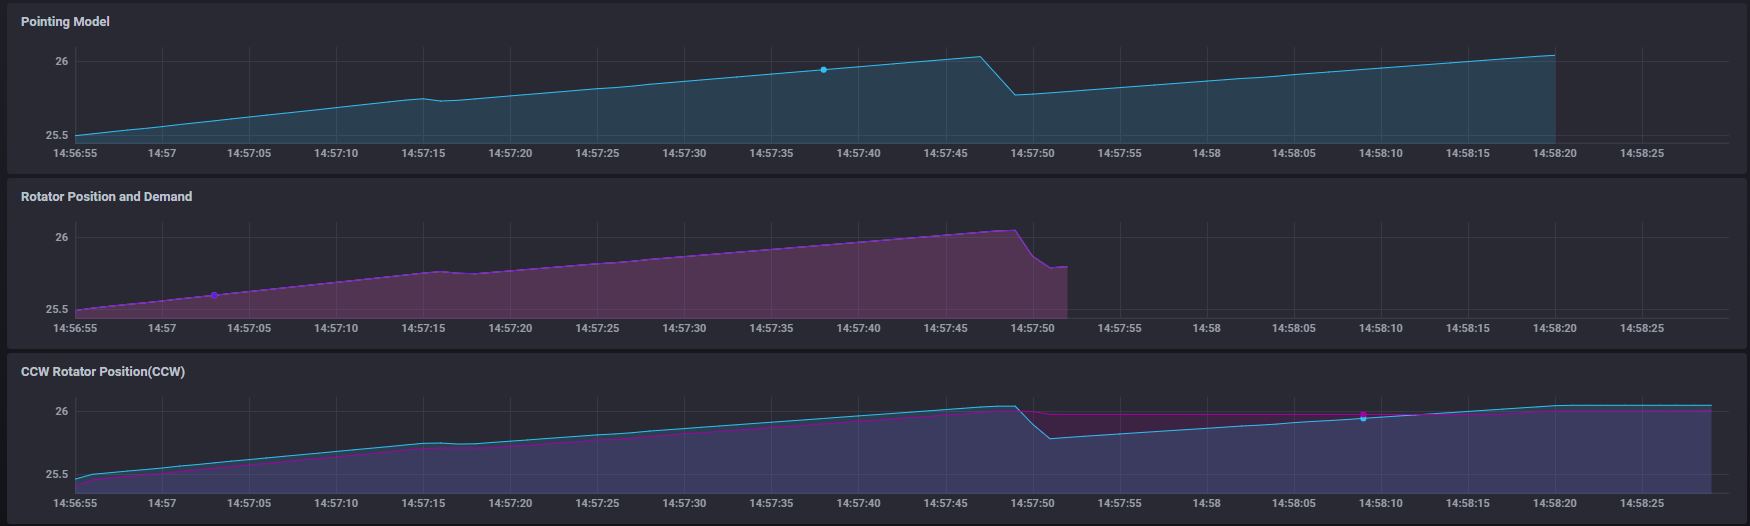
\includegraphics[width=5.20833in]{jira_imgs/1088.png}\\
\url{https://chronograf-summit-efd.lsst.codes/sources/1/dashboards/6?tempVars\%5Btest_start\%5D=START\%20-\%20Rotator\%20Night\%20Observing\%20Integration\%20Test\&tempVars\%5Btest_end\%5D=END\%20-\%20Rotator\%20Night\%20Observing\%20Integration\%20Test\&lower=now\%28\%29\%20-\%2015m}

\medskip }
\end{minipage} \\ \cdashline{2-2}

 & Status: \textbf{ Initial Pass } \\ \hline

36 & Description \\
 & \begin{minipage}[t]{15cm}
{\footnotesize
\smallskip
Bring the Camera Rotator and the Pointing Component to the Enabled
State.

\medskip }
\end{minipage}
\\ \cdashline{2-2}


 & Expected Result \\
 & \begin{minipage}[t]{15cm}{\footnotesize
\smallskip
The Camera Rotator and Pointing Component are in the Enabled State.

\medskip }
\end{minipage} \\ \cdashline{2-2}

 & Actual Result \\
 & \begin{minipage}[t]{15cm}{\footnotesize
\smallskip
The Camera Rotator and CCW were correctly transitioned into the Enabled
state

\medskip }
\end{minipage} \\ \cdashline{2-2}

 & Status: \textbf{ Initial Pass } \\ \hline

37 & Description \\
 & \begin{minipage}[t]{15cm}
{\footnotesize
\smallskip
Send a \emph{trackStart} command to the rotator.

\medskip }
\end{minipage}
\\ \cdashline{2-2}


 & Expected Result \\
 & \begin{minipage}[t]{15cm}{\footnotesize
\smallskip
The Camera Rotator transitions from the Enabled/Stationary state to the
Enabled/SlewingAndTracking state.

\medskip }
\end{minipage} \\ \cdashline{2-2}

 & Actual Result \\
 & \begin{minipage}[t]{15cm}{\footnotesize
\smallskip
The Camera Rotator and CCW both successfully transitioned into the
SlewingAndTracking sub-state.

\medskip }
\end{minipage} \\ \cdashline{2-2}

 & Status: \textbf{ Initial Pass } \\ \hline

38 & Description \\
 & \begin{minipage}[t]{15cm}
{\footnotesize
\smallskip
The Scheduler commands the Pointing component to track simulated by a
table written in the Jupyter notebook.\\[2\baselineskip]

\medskip }
\end{minipage}
\\ \cdashline{2-2}


 & Expected Result \\
 & \begin{minipage}[t]{15cm}{\footnotesize
\smallskip
The Camera Rotator begins to track.

\medskip }
\end{minipage} \\ \cdashline{2-2}

 & Actual Result \\
 & \begin{minipage}[t]{15cm}{\footnotesize
\smallskip
{We started having more GUI problems; The GUI kept crashing and at
different points during each attempt.}

\medskip }
\end{minipage} \\ \cdashline{2-2}

 & Issues found executing this step:  \\
 & \begin{minipage}[t]{13cm}{\footnotesize
\smallskip
\href{https://jira.lsstcorp.org/browse/FRACAS-26}{FRACAS-26}~~Camera Rotator GUI Crash

\medskip }
\end{minipage} \\ \cdashline{2-2}
 & Status: \textbf{ Fail } \\ \hline

39 & Description \\
 & \begin{minipage}[t]{15cm}
{\footnotesize
\smallskip
Verify that the Camera Rotator is following the look up table of visits
one after the other by looking at chronograf.

\medskip }
\end{minipage}
\\ \cdashline{2-2}


 & Expected Result \\
 & \begin{minipage}[t]{15cm}{\footnotesize
\smallskip
After one observation is performed, the Camera Rotator begins the track
of the next target right after the last active visit.

\medskip }
\end{minipage} \\ \cdashline{2-2}

 & Actual Result \\
 & \begin{minipage}[t]{15cm}{\footnotesize
\smallskip
Deviation: We had to include \emph{stopTracking} commands in between
each track in order to complete the full test.

\medskip }
\end{minipage} \\ \cdashline{2-2}

 & Issues found executing this step:  \\
 & \begin{minipage}[t]{13cm}{\footnotesize
\smallskip
\href{https://jira.lsstcorp.org/browse/FRACAS-26}{FRACAS-26}~~Camera Rotator GUI Crash

\medskip }
\end{minipage} \\ \cdashline{2-2}
 & Status: \textbf{ Fail } \\ \hline

40 & Description \\
 & \begin{minipage}[t]{15cm}
{\footnotesize
\smallskip
Send a \emph{stopTracking} command to the pointing component.

\medskip }
\end{minipage}
\\ \cdashline{2-2}


 & Expected Result \\
 & \begin{minipage}[t]{15cm}{\footnotesize
\smallskip
The pointing component stops sending \emph{track} commands.~

\medskip }
\end{minipage} \\ \cdashline{2-2}

 & Actual Result \\
 & \begin{minipage}[t]{15cm}{\footnotesize
\smallskip
The pointing component stopped sending \emph{track} commands.

\medskip }
\end{minipage} \\ \cdashline{2-2}

 & Status: \textbf{ Initial Pass } \\ \hline

41 & Description \\
 & \begin{minipage}[t]{15cm}
{\footnotesize
\smallskip
Send a \emph{stop} command to the Camera Rotator.

\medskip }
\end{minipage}
\\ \cdashline{2-2}


 & Expected Result \\
 & \begin{minipage}[t]{15cm}{\footnotesize
\smallskip
The Camera Rotator and CCW stop their rotation.

\medskip }
\end{minipage} \\ \cdashline{2-2}

 & Actual Result \\
 & \begin{minipage}[t]{15cm}{\footnotesize
\smallskip
A \emph{stop} command was sent to the CCW first when the
\emph{stopTracking} command was sent to the pointing component and then
a \emph{stop} command was sent to the Camera Rotator. This order was
established due to sensitivities seen with the CCW to receive
\emph{stop} commands after the pointing component stopped sending the
\emph{track} commands.

\medskip }
\end{minipage} \\ \cdashline{2-2}

 & Status: \textbf{ Initial Pass } \\ \hline

\end{longtable}


\newpage
\appendix
%Make sure lsst-texmf/bin/generateAcronyms.py is in your path
\section{Acronyms used in this document}\label{sec:acronyms}
\addtocounter{table}{-1}
\begin{longtable}{p{0.145\textwidth}p{0.8\textwidth}}\hline
\textbf{Acronym} & \textbf{Description}  \\\hline

CR & Change Request \\\hline
CSV & Comma Separated Values \\\hline
GUI & Graphical User Interface \\\hline
IS & Interface Scientist \\\hline
LSST & Large Synoptic Survey Telescope \\\hline
PMCS & Project Management Controls System \\\hline
SLAC & SLAC National Accelerator Laboratory (formerly Stanford Linear Accelerator Center; SLAC is now no longer an acronym) \\\hline
\end{longtable}


\end{document}
